\chapter{}


\section{Ingeniería de requisitos}

En esta sección hablamos, en primer lugar, de los principales actores implicados en el sistema y de sus necesidades, tras lo cual, mostramos los requisitos funcionales, no funcionales y de información del sistema.

\subsection{Descripción de los implicados.}

Los principales implicados en el sistema son los profesores y los estudiantes.

\begin{tabular}{|p{3cm}|p{4cm}|p{2cm}|p{6cm}|}
\hline
{\bf Nombre } & {\bf Descripción } & {\bf Tipo } & {\bf  Responsabilidad}\\
\hline
{ Estudiante } & { Usuario de Telegram que además está apuntado a un curso en la plataforma Moodle con rol de estudiante.} & { Usuario producto. } & { Acceso a información relacionada con los cursos en los que se encuentra apuntado, genera dudas y  asiste a tutorías.} \\
\hline
{ Profesor } & {  Usuario de Telegram apuntado a un curso en la plataforma Moodle con rol de profesor.} & { Usuario producto } & { Responsable de una asignatura y de sus tutorías.} \\
\hline
{ Usuario registrado } & {  Usuario de Telegram que se ha identificado respecto al \textit{bot} y éste lo tiene registrado.} & { Usuario producto } & { Acceso a funciones comunes para todos los usuarios que se registren en el \textit{bot}. } \\
\hline
{ Usuario sin identificar } & {  Usuario de telegram que no se ha dado de alta respecto al \textit{bot}.} & { Usuario producto } & { } \\
\hline
{ Usuario chat grupal Telegram} & {  Cualquier usuario de un chat de telegram asociado a un curso.} & { Usuario producto } & { Realiza consultas al \textit{bot} con interacciones tipo usuario pregunta, bot responde, fin interacción.} \\
\hline

\end{tabular}



\textbf{Estudiante}

\begin{table}[H]
\begin{tabular}{|c|p{10cm}|}
\hline
{ Descripción } & {Usuario registrado en cursos de un servidor de Moodle con rol de estudiante, que accede a información de estos cursos, tales como entregas que ha realizado o que tiene que realizar y a su vez produce información relacionada con los cursos como peticiones a tutorías. }\\
\hline 
{ Tipo } & { Utiliza el sistema de forma directa y aporta información  adicional relacionada con los cursos.}  \\
\hline
{ Responsabilidad } & { Acceder a la información del curso.
Ver notas de sus entregas en un curso.
Solicitar tutorías.
Plantear dudas.
}  \\
\hline
{ Criterios de éxito }& { Que el sistema le permita realizar sus actividades de la forma más sencilla posible.}\\
\hline
{ Implicación }& { Utilizará el sistema de forma activa.} \\
\hline
{ Comentarios/Cuestiones }& { } \\
\hline

\end{tabular}
\end{table}

\textbf{Usuario registrado}

\begin{table}[H]
\begin{tabular}{|c|p{10cm}|}
\hline
{ Descripción } & {Cualquier usuario que se ha registrado con respecto al bot  }\\
\hline 
{ Tipo } & { Utiliza el sistema de forma directa y aporta información  adicional relacionada con los cursos.}  \\
\hline
{ Responsabilidad } & {
Plantear dudas.
}  \\
\hline
{ Criterios de éxito }& { Poder tener un manejo de las dudas asociadas a un curso lo más simple posible.}\\
\hline
{ Implicación }& { Utilizará el sistema de forma activa.} \\
\hline
{ Comentarios/Cuestiones }& { Representa las actividades comunes que pueden realizar utilizando el bot los profesores y estudiantes} \\
\hline

\end{tabular}
\end{table}

\newpage
\textbf{Profesor}
\begin{table}[H]
\medskip 
\begin{tabular}{|c|p{10cm}|}
\hline
{ Descripción } & {Usuario registrado en cursos de un servidor de Moodle con rol de profesor que está a cargo de la gestión de una serie de asignaturas, gestiona todo lo relacionado con éstas tal y como recursos (pdfs, urls, imágenes..), entregas, dudas y tutorías.}\\
\hline
{ Tipo } & { Utiliza el sistema de forma directa y aporta información “indirecta” o adicional relacionada con los cursos.}  \\
\hline
{ Responsabilidad } & { Gestionar la información del curso.
Ver entregas de un curso.
Realizar entregas de un curso.
Gestión tutorias.
Plantear dudas.}  \\
\hline
{ Criterios de éxito }& { Que el sistema le permita realizar sus actividades de la forma más sencilla posible.}\\
\hline
{ Implicación }& { Utilizará el sistema de forma activa.} \\
\hline
{ Comentarios/Cuestiones }& { } \\
\hline


\end{tabular}
\end{table}


\textbf{Usuario chat grupal Telegram}

\begin{table}[H]
\begin{tabular}{|c|p{10cm}|}
\hline
{ Descripción } & {Cualquier usuario de un chat de Telegram en cuyo interior se encuentre el \textit{bot} y que este chat esté asociado a un curso de Moodle. }\\
\hline 
{ Tipo } & { Utiliza el sistema para obtener información general de un curso.}  \\
\hline
{ Responsabilidad } & { Aportar información de interés general para el  curso.
Consultar información general del curso: preguntar fecha de próximas entregas de una asignatura, consultar dudas del curso.
}  \\
\hline
{ Criterios de éxito }& { El sistema muestra claramente que acciones puede realizar y cual será el resultado de estas.}\\
\hline
{ Implicación }& { Utilizará el sistema de forma activa.} \\
\hline
{ Comentarios/Cuestiones }& { Al ser un chat donde participa mucha gente, las interacciones del \textit{bot} tienen que ser breves y contundentes para evitar que genere ruido.} \\
\hline

\end{tabular}
\end{table}

\subsubsection{Necesidades principales de los implicados}



\begin{table}[H]
\medskip 
\begin{tabular}{|p{2cm}|p{1.6cm}|p{2.5cm}|p{3.5cm}| p{4cm}|}
\hline
{\bf Necesidad } & {\bf Prioridad } & {\bf Problema } & {\bf  Solución actual.} & {\bf  Solución propuesta.}\\
\hline
{ Petición tutorías }& { Alta } & { Poder solicitar una tutoría a un profesor de una asignatura } & {Buscar el correo electrónico del profesor responsable de la asignatura y mandarle un correo electrónico al profesor } & { Solicitar al \textit{bot} una tutoría para una asignatura y éste guarda las solicitudes y notifica al profesor}\\
\hline
{ Gestionar tutorías }& { Alta } & { Gestionar las tutorías de las que es responsable y conocer quienes quieren asistir a ellas } & {Llevar una lista mentalmente o en el correo de estudiantes que han solicitado asistir a una de sus tutorías} & { Permitir al profesor definir tutorías a través del \textit{bot} visibles para los estudiantes de sus cursos que pueden realizar solicitudes a ellas llevándose un recuento de las solicitudes realizadas}\\
\hline
{ Resolver dudas curso }& { Alta } & { Resolver una duda sobre cómo actuar ante un problema surgido durante el desarrollo de las actividades de un curso }& { Buscar el correo del profesor, mandarle correo electrónico ó contactar con algún conocido y preguntarle } & { Guardar la duda del usuario y permitir que mediante el \textit{bot} los usuarios de un curso aporten soluciones.}\\
\hline
{ Conocer información acerca de las entregas  } & { Alta} & { Poder conocer el estado de las entregas para un curso}& { Acceder a Moodle y para cada curso en el que se está matriculado ver si hay alguna actividad abierta } & {Indicando al \textit{bot} que quiere saber las entregas de un curso, cuales de ellas están abiertas, si alguna tiene notas..} \\
\hline


\end{tabular}
\end{table}
\newpage
\subsection{Especificación de requisitos}

\subsubsection{Requisitos funcionales}

Debido a que se pueden incluir muchas funcionalidades y que el tiempo es limitado, las funciones a implementar por el sistema para cubrir las necesidades de los usuarios son:

\renewcommand{\labelenumii}{\theenumii}
\renewcommand{\theenumii}{\theenumi.\arabic{enumii}.}


\begin{itemize}


\item \textbf{RF-1} Acceso usuarios.
	\begin{itemize}
	\item \textbf{RF-1.1} El sistema debe permitir a un usuario registrado en la instancia de moodle utilizar el \textit{bot}.
	\end{itemize}

\item \textbf{RF-2} El \textit{bot} debe permitir a los usuarios que lo usan especificar el curso sobre el cual tendrán efecto sus acciones.
	
\item \textbf{RF-3} El \textit{bot} debe dar a un usuario información acerca de las entregas para los cursos a los cuales tiene acceso el usuario:
\begin{itemize}
	\item\textbf{RF-3.1} Proporcionar a un estudiante información acerca de las entregas que se encuentran abiertas tales como: la fecha de entrega, descripción de qué hay que hacer en la entrega si la hubiera o cuántos días faltan para la entrega.
	
	\item\textbf{RF-3.2} Información acerca de las notas que tiene para las entregas.

	\end{itemize}	


\item \textbf{RF-4} Gestión de las dudas de un curso.
\begin{itemize}

	\item\textbf{RF-4.1} El sistema debe permitir a un profesor o estudiante crear dudas relacionadas con un curso.
	\item\textbf{RF-4.2} El sistema debe permitir al usuario que crea la duda o al profesor marcar como resuelta una duda.
	\item\textbf{RF-4.3} Cualquier usuario con acceso al curso debe poder ver las dudas para ese curso.
	\item\textbf{RF-4.4} Cualquier usuario con acceso al curso debe poder aportar respuestas a una duda.
	\end{itemize}

\item \textbf{RF-5} Gestión de tutorias.
\begin{itemize}

	\item\textbf{RF-5.1} El profesor de un curso puede:
	\begin{itemize}

	\item\textbf{RF-5.1.1} Definir las tutorías para ese curso.
	\item\textbf{RF-5.1.2} Aprobar o denegar las peticiones que reciba de tutorías.
	\item\textbf{RF-5.1.3} Conocer la cola de peticiones aprobadas para una tutoría.
	\end{itemize}
	
	\item\textbf{RF-5.2} El estudiante de un curso puede:
	\begin{itemize}
	\item\textbf{RF-5.2.1} Conocer las tutorías del profesor asociado a  un curso.
	\item\textbf{RF-5.2.2} Solicitar asistir a una tutoría de un curso.
	\item\textbf{RF-5.2.3} Conocer el estado de sus solicitudes.
	\end{itemize}	
	\end{itemize}


\item \textbf{RF-6} Chats grupales de Telegram.
\begin{itemize}

	\item\textbf{RF-6.1} El profesor de un curso puede asociar un chat de grupo de Telegram a un curso de los que es responsable.
	\item\textbf{RF-6.2} El bot tiene que aportar información general relevante para un curso en un chat grupal.
	\begin{itemize}

	\item\textbf{RF-6.2.1} Fechas de las entregas abiertas para el curso asociado al chat.
	\item\textbf{RF-6.2.2} Información acerca de una entrega en concreto.
	\item\textbf{RF-6.2.3} Dudas actuales asociadas con el curso.
	\item\textbf{RF-6.2.4} Tutorías del profesor.
	\end{itemize}
	
	\end{itemize}


\end{itemize}



\subsubsection{Requisitos no funcionales}


\subsubsection*{Empaquetamiento}
\begin{itemize}

\item \textbf{RNF-1} El sistema debe poder aprovisionarse automáticamente.
\item \textbf{RNF-2} El sistema debe poder desplegarse automáticamente a través de ssh.
\end{itemize}
\subsubsection*{Seguridad}
\begin{itemize}
\item \textbf{RNF-3} Toda la comunicación entre el sistema y la instancia de Moodle debe estar cifrada utilizando ssl.
\end{itemize}

\subsubsection*{Interfaz}
\begin{itemize}
\item \textbf{RNF-4} El sistema debe proporcionar al usuario menús gráficos para toda acción que requiere más de dos pasos.
\end{itemize}
\subsubsection*{Legales}
\begin{itemize}
\item \textbf{RNF-5} El \textit{bot} tiene que tener una licencia libre. 

\end{itemize}

\subsubsection{Requisitos de información}

\begin{itemize}
\item \textbf{RI-1.} Usuario Moodle.\\
Almacenamos información de un usuario  de Moodle.\\
\textbf{Contenido}: email, token, id\_moodle
\item \textbf{RI-2.} Cursos.\\
Información sobre un curso de Moodle.
\\
\textbf{Contenido}: nombre, id\_moodle\_curso
\item \textbf{RI-3.} Usuario Telegram.\\
Datos asociados a un usuario de Telegram.
\\
\textbf{Contenido}: nombre\_usuario, id\_telegram
\item \textbf{RI-4.} Cursos.\\
Información sobre un curso de Moodle.
\\
\textbf{Contenido}: nombre, id\_moodle\_curso
\item \textbf{RI-5.} Dudas.\\
Datos de las dudas de un curso.
\\
\textbf{Contenido}: contenido
\item \textbf{RI-6.} Respuestas.\\
Datos de las respuestas que tienen las dudas.
\\
\textbf{Contenido}: contenido.
\item \textbf{RI-7.} Tutorías.\\
Información asociada a las tutorías de un profesor.
\\
\textbf{Contenido}: día semana, hora.
\item \textbf{RI-8.} Tutorías.\\
Información asociada a las tutorías de un profesor.
\\
\textbf{Contenido}: día semana, hora.

\item \textbf{RI-9.} Peticiones.\\
Datos relacionados con las peticiones a tutorías.
\\
\textbf{Contenido}: hora solicitud.
\item \textbf{RI-10.} Chat Telegram.\\
Datos asociados a un chat de Telegram.
\\
\textbf{Contenido}: nombre\_chat, id\_chat\_telegram

\end{itemize}


\newpage

\subsection{Casos de uso}

En esta sección procedemos a mostrar los casos de uso más relevantes del sistema. Primero mostramos el diagrama de casos de uso para después desarrollar algunos de manera más básica y otros de forma  más extendida.

\subsection{Diagrama casos uso}

A través diagrama de casos de usos podemos obtener una primera aproximación de como interaccionan con el sistema los distintos actores  que hemos descrito anteriormente. 
\begin{figure}[H] %con el [H] le obligamos a situar aquí la figura
\centering
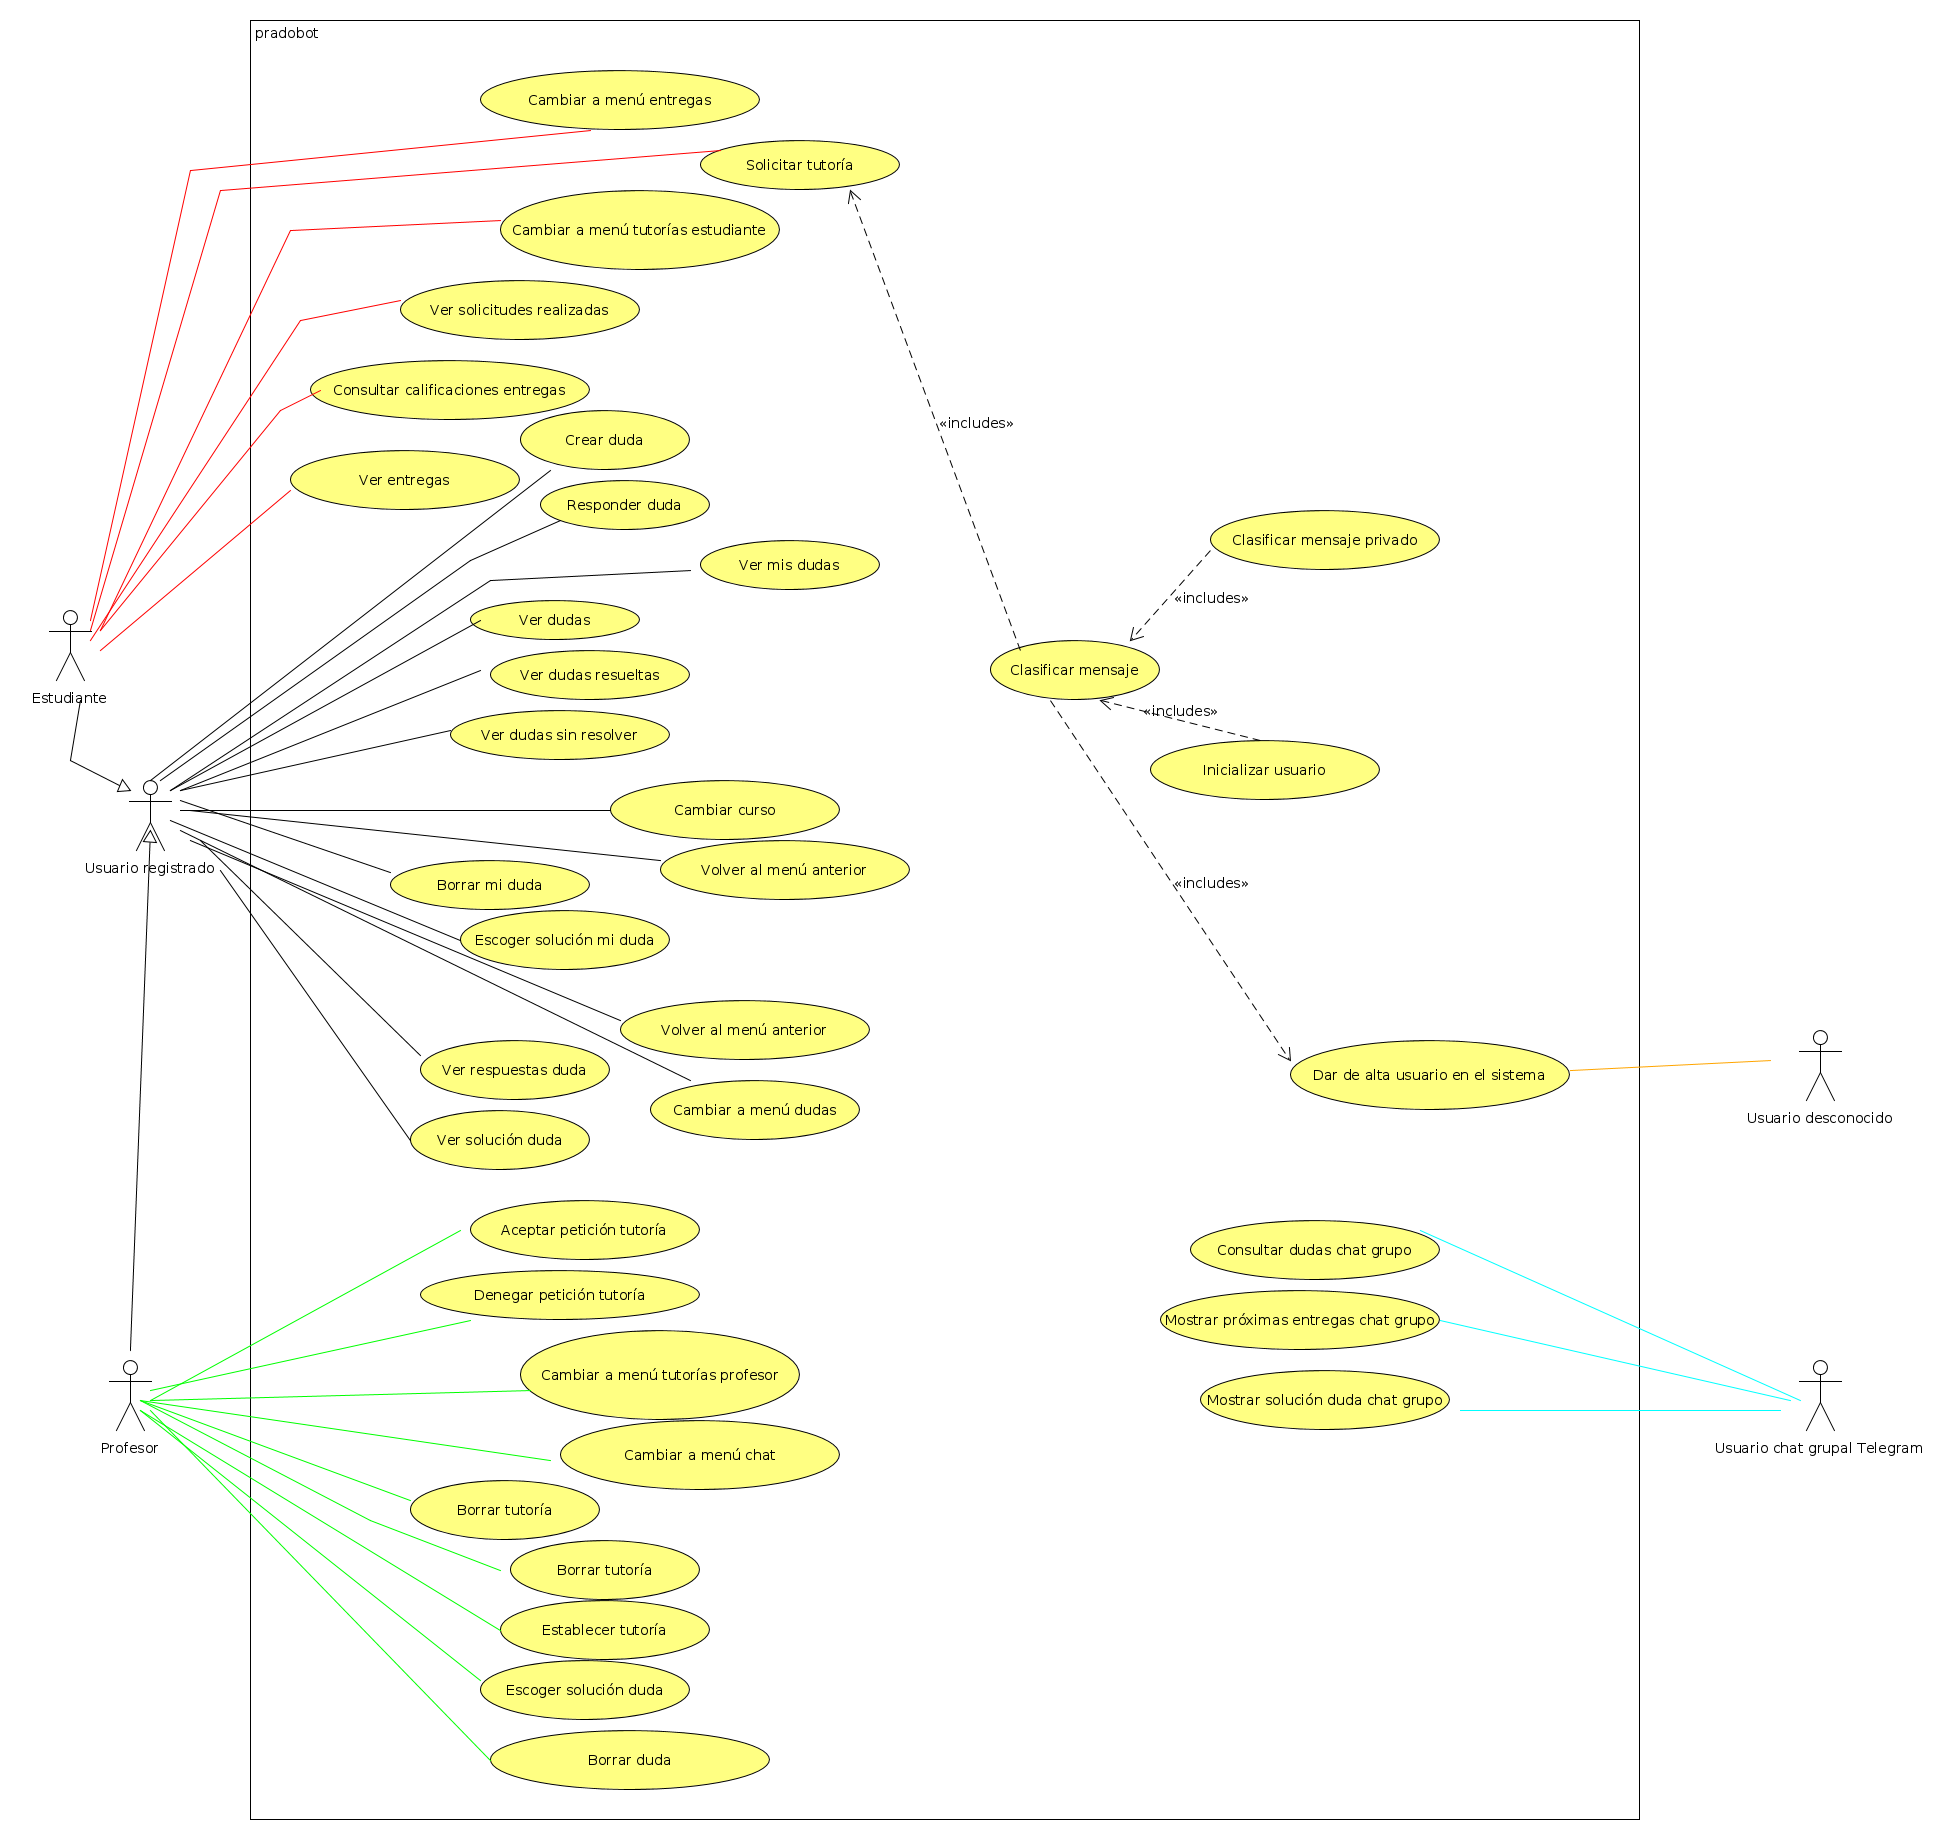
\includegraphics[scale=0.2]{imagenes/diagramas/diagrama_caso_uso.png}  %el parámetro scale permite agrandar o achicar la imagen. En el nombre de archivo puede especificar directorios

\caption{Diagrama de los casos de uso más relevantes del sistema}\label{figura10}
\end{figure}

Podemos observar las funciones comunes que comparten todos los usuarios registrados del sistema, así como las que son especificas de cada rol. Por ejemplo, algo exclusivo del profesor es el establecimiento de las tutorías, mientras que algo único que puede hacer el estudiante es solicitarlas.


\subsection{Descripción casos uso}

He optado por realizar dos tipos de CUs unos más cercanos a los CU Reales, que muestran algunos detalles más cercanos al diseño y otros, bastante más abstractos, cuyo enfoque está en mostrar la interacción del usuario con el programa. El objetivo, es que haya equilibrio entre abstracción y las peculiaridades de un programa tipo bot, cuyo funcionamiento depende fuertemente del contexto en el que se recibe un mensaje del usuario.

\begin{table}[H]

\begin{tabular}{|c|m{10cm}|}
\hline\rowcolor{Gray}
{\bf CU-1.1 } & { Clasificar mensaje.}\\
\hline
{\bf Actores } & { Estudiante, Profesor} \\
\hline\rowcolor{Gray}
{\bf Tipo } & { Primario,  Real} \\
\hline
{\bf Referencias }& {CU-1.2 (Clasificar mensaje privado)} \\
\hline\rowcolor{Gray}
{\bf Precondición }& {Bot haya recibido un mensaje} \\
\hline
{\bf Postcondición }& {}\\
\hline\rowcolor{Gray}
{\bf Autor }& { Luis Gil Guijarro}  \\
\hline
{\bf Versión }& { 1.0} \\
\hline\rowcolor{Gray}
{\bf Fecha }& { 10-05-17} \\
\hline
\end{tabular}

\end{table}

\begin{table}[H]

\begin{tabular}{|m{10cm}|}
\hline\rowcolor{Gray}
{\bf Propósito}\\
\hline
{Clasificar un mensaje recibido desde Telegram para determinar si procede de un chat individual o de uno grupal.} \\
\hline

\end{tabular}


\end{table}

\begin{table}[H]

\begin{tabular}{|m{10cm}|}
\hline\rowcolor{Gray}
{\bf Resumen}\\
\hline
{El bot recibe un mensaje y lo clasifica dependiendo de si procede de un chat privado o de uno grupal.} \\
\hline

\end{tabular}



\end{table}

    \begin{table}[!ht]
	\begin{tabular}{|l|l|l|l|}
	  \hline\rowcolor{Gray}
	  \multicolumn{4}{|c|}{{\bf Curso normal}}
	  \\ \hline
	  \multicolumn{2}{|c|}{{\bf Actor}} & \multicolumn{2}{c|}{{\bf Sistema}}
	  \\ \hline

	  &
	  &
	  {\textbf 1} &
	  \begin{tabular}[c]{@{}l@{}}
	    El bot recibe el mensaje.
	  \end{tabular}
	  \\ \hline	  &
	  &
	  {\textbf 2} &
	  \begin{tabular}[c]{@{}l@{}}
	    El bot comprueba si el mensaje procede de un\\ chat grupal o de uno privado.
	  \end{tabular}
	  \\ \hline	  &
	  &
	  {\textbf 3} &
	  \begin{tabular}[c]{@{}l@{}}
	    El bot clasifica el mensaje como privado.
	  \end{tabular}
	  \\ \hline	  &
	  &
	  {\textbf 4} &
	  \begin{tabular}[c]{@{}l@{}}
	    Incluir( CU-1.2, Clasificar mensaje privado)
	  \end{tabular}
	  \\ \hline	  
	\end{tabular}
	\caption{Curso normal de CU-1.1. Clasificar mensaje.}
	\label{table:cn_cu_1.1}
    \end{table}

    \begin{table}[!ht]
	\begin{tabular}{|l|l|l|l|}
	  \hline\rowcolor{Gray}
	  \multicolumn{2}{|c|}{{\bf Cursos alternos}}
	  \\ \hline
	  {\textbf 3a} & 
	  \begin{tabular}[c]{@{}l@{}}
	    El bot clasifica el mensaje como grupal\\ Incluir( CU-1.4, Clasificar mensaje grupal) \\Fin CU.
	  \end{tabular} 
	  
	  
	  \\ \hline
	\end{tabular}
	\caption{Cursos alternos de CU-1.1. Clasificar mensaje.}
	\label{table:ca_cu_1.1}
    \end{table}
    
    
%%%%%%%%%%%%%%%%%%%%%%%%%%%%%%%%%%%%%%%%%%%%%%%%%%%%%%%
    
\begin{table}[!ht]

\begin{tabular}{|c|m{10cm}|}
\hline\rowcolor{Gray}
{\bf CU-1.2 } & { Clasificar mensaje privado}\\
\hline
{\bf Actores } & { Estudiante, Profesor} \\
\hline\rowcolor{Gray}
{\bf Tipo } & { Primario, Real} \\
\hline
{\bf Referencias }& {CU-1.3 (Inicializar usuario)} \\
\hline\rowcolor{Gray}
{\bf Precondición }& {El bot haya recibido un mensaje. El mensaje debe proceder desde un chat privado de Telegram} \\
\hline
{\bf Postcondición }& {}\\
\hline\rowcolor{Gray}
{\bf Autor }& { Luis Gil Guijarro}  \\
\hline
{\bf Versión }& { 1.0} \\
\hline\rowcolor{Gray}
{\bf Fecha }& { 10-05-17} \\
\hline
\end{tabular}

\end{table}

\begin{table}[!ht]

\begin{tabular}{|m{10cm}|}
\hline\rowcolor{Gray}
{\bf Propósito}\\
\hline
{Clasificar un mensaje procedente de un chat privado} \\
\hline

\end{tabular}


\end{table}

\begin{table}[!ht]

\begin{tabular}{|m{10cm}|}
\hline\rowcolor{Gray}
{\bf Resumen}\\
\hline
{El bot recibe un mensaje determinando el tipo de usuario que le manda el mensaje y si es la primera vez que recibe un mensaje de este usuario } \\
\hline

\end{tabular}



\end{table}

    \begin{table}[!ht]
	\begin{tabular}{|l|l|l|l|}
	  \hline\rowcolor{Gray}
	  \multicolumn{4}{|c|}{{\bf Curso normal}}
	  \\ \hline
	  \multicolumn{2}{|c|}{{\bf Actor}} & \multicolumn{2}{c|}{{\bf Sistema}}
	  \\ \hline

	  &
	  &
	  {\textbf 1} &
	  \begin{tabular}[c]{@{}l@{}}
	    Obtiene todos los usuarios\\ que han usuado el\\ bot desde que éste empezó a funcionar
	  \end{tabular}
	  	  \\ \hline

	  &
	  &
	  {\textbf 2} &
	  \begin{tabular}[c]{@{}l@{}}
	    Obtiene al usuario del mensaje.
	  \end{tabular}
	  \\ \hline	  &
	  &
	  {\textbf 3} &
	  \begin{tabular}[c]{@{}l@{}}
	    Comprueba si el usuario que le ha mandado el mensaje\\ está entre ellos.
	  \end{tabular}
	  \\ \hline	  &
	  &
	  {\textbf 4} &
	  \begin{tabular}[c]{@{}l@{}}
	    Comprueba si ha acabo de procesarse el último\\ mensaje que envió el usuario.
	  \end{tabular}
	  \\ \hline	  &
	  &
	  {\textbf 5} &
	  \begin{tabular}[c]{@{}l@{}}
	    Obtiene el menú devuelto por el último menú\\ utilizado por el usuario.
	  \end{tabular}
	  \\ \hline	  &
	  &
	  {\textbf 6} &
	  \begin{tabular}[c]{@{}l@{}}
	    Pasa el nuevo mensaje del usuario al\\ menú devuelto.
	  \end{tabular}
	  \\ \hline
	\end{tabular}
	\caption{Curso normal de CU-1.2. Clasificar mensaje privado.}
	\label{table:cn_cu_1.2}
    \end{table}

    \begin{table}[!ht]
	\begin{tabular}{|l|l|l|l|}
	  \hline\rowcolor{Gray}
	  \multicolumn{2}{|c|}{{\bf Cursos alternos}}
	  \\ \hline
	  {\textbf 3a} & 
	  \begin{tabular}[c]{@{}l@{}}
	    	    El usuario no le ha mandado un \\mensaje al bot desde que éste  \\ empezó a funcionar\\. Incluir (CU-1.3, inicializar usuario)
 . Fin CU.
	  \end{tabular} 
	  \\ \hline
	  {\textbf 4a} & 
	  \begin{tabular}[c]{@{}l@{}}
	    La acción que ejecutó el usuario\\ en su último mensaje no se \\ ha acabado de ejecutar\\. Bot le pide que espere . Fin CU.
	  \end{tabular} 
	  \\ \hline
	\end{tabular}
	\caption{Cursos alternos de CU-1.2. Clasificar mensaje privado.}
	\label{table:ca_cu_1.2}
    \end{table}
    


%%%%%%%%%%%%%%%%%%%%%



\begin{table}[!ht]

\begin{tabular}{|c|m{10cm}|}
\hline\rowcolor{Gray}
{\bf CU-1.3 } & {Inicializar usuario}\\
\hline
{\bf Actores } & { Estudiante, Profesor} \\
\hline\rowcolor{Gray}
{\bf Tipo } & { Primario, Real} \\
\hline
{\bf Referencias }& {} \\
\hline\rowcolor{Gray}
{\bf Precondición }& {El usuario que le manda el mensaje al bot no le haya mandado un mensaje anteriormente desde que éste empezó a ejecutarse} \\
\hline
{\bf Postcondición }& {El usuario será añadido a la lista de usuarios que están utilizando el bot}\\
\hline\rowcolor{Gray}
{\bf Autor }& { Luis Gil Guijarro}  \\
\hline
{\bf Versión }& { 1.0} \\
\hline\rowcolor{Gray}
{\bf Fecha }& { 10-05-17} \\
\hline
\end{tabular}

\end{table}

\begin{table}[!ht]

\begin{tabular}{|m{10cm}|}
\hline\rowcolor{Gray}
{\bf Propósito}\\
\hline
{Asignarle un menú de inicio al usuario que le ha mandado el mensaje} \\
\hline

\end{tabular}


\end{table}

\begin{table}[!ht]

\begin{tabular}{|m{10cm}|}
\hline\rowcolor{Gray}
{\bf Resumen}\\
\hline
{El bot determina si el usuario está registrado en el sistema y le asigna un menú de inicio. } \\
\hline

\end{tabular}



\end{table}

    \begin{table}[!ht]
	\begin{tabular}{|l|l|l|l|}
	  \hline\rowcolor{Gray}
	  \multicolumn{4}{|c|}{{\bf Curso normal}}
	  \\ \hline
	  \multicolumn{2}{|c|}{{\bf Actor}} & \multicolumn{2}{c|}{{\bf Sistema}}
	  \\ \hline

	  &
	  &
	  {\textbf 1} &
	  \begin{tabular}[c]{@{}l@{}}
	    Bot comprueba si el usuario está registrado\\ en el sistema.
	  \end{tabular}
	  \\ \hline	  &
	  &
	  {\textbf 2} &
	  \begin{tabular}[c]{@{}l@{}}
	    El bot obtiene una lista de cursos en los que\\ se encuentra matriculado el usuario.
	  \end{tabular}
	  \\ \hline	  &
	  &
	  {\textbf 3} &
	  \begin{tabular}[c]{@{}l@{}}
	    El bot asigna como curso activo del usuario\\ al primer curso de la lista.
	  \end{tabular}
	  \\ \hline	  &
	  &
	  {\textbf 4} &
	  \begin{tabular}[c]{@{}l@{}}
	    El bot obtiene el menú inicial del profesor.
	  \end{tabular}
	  \\ \hline	  &
	  &
	  {\textbf 5} &
	  \begin{tabular}[c]{@{}l@{}}
	    El bot le muestra al usuario el menú\\ principal del profesor.
	  \end{tabular}
	  \\ \hline

	\end{tabular}
	\caption{Curso normal de CU-1.3. Inicializar usuario.}
	\label{table:cn_cu_1.3}
    \end{table}

    \begin{table}[!ht]
	\begin{tabular}{|l|l|l|l|}
	  \hline\rowcolor{Gray}
	  \multicolumn{2}{|c|}{{\bf Cursos alternos}}
	  \\ \hline
	  {\textbf 2a} & 
	  \begin{tabular}[c]{@{}l@{}}
	    El usuario no está registrado en el sistema. Obtiene\\ el menú encargado de iniciar usuarios desconocidos.\\ Muestra este menú al usuario. Fin CU.
	  \end{tabular} 
	  
	  
	  \\ \hline
	  	  {\textbf 4a} & 
	  \begin{tabular}[c]{@{}l@{}}
	    El usuario es un estudiante. Obtiene el menú inicial\\ del estudiante y se lo muestra. Fin CU.
	  \end{tabular} 
	  
	  
	  \\ \hline
	\end{tabular}
	\caption{Cursos alternos de CU-1.3. Inicializar usuario.}
	\label{table:ca_cu_1.3}
    \end{table}
    


%%%%%%%%%%%%%%%%%%%%%%%%%%%%%%%%%%%%%%%%%%%




\begin{table}[!ht]

\begin{tabular}{|c|m{10cm}|}
\hline\rowcolor{Gray}
{\bf CU-1.4 } & { Cambiar curso.}\\
\hline
{\bf Actores } & { Usuario Registrado} \\
\hline\rowcolor{Gray}
{\bf Tipo } & { Primario, Real} \\
\hline
{\bf Referencias }& {CU-1.1 (Clasificar mensaje)} \\
\hline\rowcolor{Gray}
{\bf Precondición }& {} \\
\hline
{\bf Postcondición }& {El usuario habrá cambiado el curso sobre el que actúan los mensajes que le envíe al bot.}\\
\hline\rowcolor{Gray}
{\bf Autor }& { Luis Gil Guijarro}  \\
\hline
{\bf Versión }& { 1.0} \\
\hline\rowcolor{Gray}
{\bf Fecha }& { 10-05-17} \\
\hline
\end{tabular}

\end{table}

\begin{table}[!ht]

\begin{tabular}{|m{10cm}|}
\hline\rowcolor{Gray}
{\bf Propósito}\\
\hline
{Que un usuario que utilice el bot pueda variar el curso sobre el cual actúan sus mensajes} \\
\hline

\end{tabular}


\end{table}

\begin{table}[!ht]

\begin{tabular}{|m{10cm}|}
\hline\rowcolor{Gray}
{\bf Resumen}\\
\hline
{El usuario selecciona en el menú que le esté mostrando el bot, que desea cambiar de curso. El bot le muestra los cursos accesibles para el usuario, el usuario escoge uno y el bot cambia el curso del usuario.} \\
\hline

\end{tabular}



\end{table}


    \begin{table}[!ht]
	\begin{tabular}{|l|l|l|l|}
	  \hline\rowcolor{Gray}
	  \multicolumn{4}{|c|}{{\bf Curso normal}}
	  \\ \hline
	  \multicolumn{2}{|c|}{{\bf Actor}} & \multicolumn{2}{c|}{{\bf Sistema}}
	  \\ \hline
	  {\textbf 1} & 
	  \begin{tabular}[c]{@{}l@{}}
	    El usuario selecciona en el\\ menú que tenga activo\\ que desea cambiar de curso.
	  \end{tabular} 
	  &
	  &
	  \\ \hline
	  &
	  &
	  {\textbf 2} &
	  \begin{tabular}[c]{@{}l@{}}
	    Incluir(CU-1.1, Clasificar mensaje)
	  \end{tabular}
	  \\ \hline
	  	  &
	  &
	  {\textbf 3} &
	  \begin{tabular}[c]{@{}l@{}}
	    El bot detecta que el usuario\\ ha pulsado cambiar de curso.
	  \end{tabular}
	  \\ \hline
	  	  	  &
	  &
	  {\textbf 4} &
	  \begin{tabular}[c]{@{}l@{}}
	    El bot obtiene todos los cursos\\ para los cuales está dado de\\ alta el usuario.
	  \end{tabular}
	  \\ \hline
	  &
	  &
	  {\textbf 5} &
	  \begin{tabular}[c]{@{}l@{}}
	    El bot muestra todos los cursos al usuario.
	  \end{tabular}
	  \\ \hline	  
	  {\textbf 6} & 
	  \begin{tabular}[c]{@{}l@{}}
	    El usuario elige\\ un curso\\.
	  \end{tabular} 
	  &
	  &
	  \\ \hline
	  &
	  &
	  {\textbf 7} &
	  \begin{tabular}[c]{@{}l@{}}
	    Incluir(CU-1.1, Clasificar mensaje)
	  \end{tabular}
	  \\ \hline	  
	  
	  	  &
	  &
	  {\textbf 8} &
	  \begin{tabular}[c]{@{}l@{}}
	    El bot identifica al curso \\seleccionado por el usuario.
	  \end{tabular}
	  \\ \hline
	  	  	  &
	  &
	  {\textbf 9} &
	  \begin{tabular}[c]{@{}l@{}}
	    El bot cambia el curso para el usuario.
	  \end{tabular}
	  \\ \hline
	  	  	  &
	  &
	  {\textbf 10} &
	  \begin{tabular}[c]{@{}l@{}}
	    El bot informa al usurio del cambio de curso.\\
	  \end{tabular}
	  \\ \hline
	\end{tabular}
	\caption{Curso normal de CU-1.4. Cambiar de curso.}
	\label{table:cn_cu_1.4}
    \end{table}



%%%%%%%%%%%%%%%%%%%%%%%%%%%%%%%%%%%%%%%%%%%%
\clearpage
\begin{table}[!ht]

\begin{tabular}{|c|m{10cm}|}
\hline\rowcolor{Gray}
{\bf CU-2 } & { Dar de alta usuario en el sistema.}\\
\hline
{\bf Actores } & { Usuario sin identificar} \\
\hline\rowcolor{Gray}
{\bf Tipo } & { Primario,  Real} \\
\hline
{\bf Referencias }& {CU-1.1 (Clasificar mensaje)} \\
\hline\rowcolor{Gray}
{\bf Precondición }& {El usuario no este registrado en el sistema.} \\
\hline
{\bf Postcondición }& {Se habrá registrado un nuevo usuario en el sistema.}\\
\hline\rowcolor{Gray}
{\bf Autor }& { Luis Gil Guijarro}  \\
\hline
{\bf Versión }& { 1.0} \\
\hline\rowcolor{Gray}
{\bf Fecha }& { 10-05-17} \\
\hline
\end{tabular}

\end{table}

\begin{table}[!ht]

\begin{tabular}{|m{10cm}|}
\hline\rowcolor{Gray}
{\bf Propósito}\\
\hline
{Para utilizar el bot es necesario que el usuario se identifique como usuario autorizado, para lo cual es necesario que pruebe que tiene acceso a los recursos de la instancia de Moodle.} \\
\hline

\end{tabular}


\end{table}

\begin{table}[!ht]

\begin{tabular}{|m{10cm}|}
\hline\rowcolor{Gray}
{\bf Resumen}\\
\hline
{El usuario manda un mensaje al bot y éste le pide que se identifique introduciendo el email y contraseña que utiliza en Moodle, el usuario los introduce y el bot registra al usuario} \\
\hline

\end{tabular}



\end{table}


    \begin{table}[!ht]
	\begin{tabular}{|l|l|l|l|}
	  \hline\rowcolor{Gray}
	  \multicolumn{4}{|c|}{{\bf Curso normal}}
	  \\ \hline
	  \multicolumn{2}{|c|}{{\bf Actor}} & \multicolumn{2}{c|}{{\bf Sistema}}
	  \\ \hline
	  {\textbf 1} & 
	  \begin{tabular}[c]{@{}l@{}}
	    El usuario manda un mensaje al bot.
	  \end{tabular} 
	  &
	  &
	  \\ \hline
	  &
	  &
	  {\textbf 2} &
	  \begin{tabular}[c]{@{}l@{}}
	    Incluir(CU-1.1, Clasificar mensaje)
	  \end{tabular}
	  \\ \hline
	  	  &
	  &
	  {\textbf 3} &
	  \begin{tabular}[c]{@{}l@{}}
	    El bot le solicita que introduzca el\\ email que utiliza en Moodle.
	  \end{tabular}
	  \\ \hline
	  	  {\textbf 4} & 
	  \begin{tabular}[c]{@{}l@{}}
	   El usuario manda un mensaje al bot\\ indicando su email.
	  \end{tabular} 
	  &
	  &
	  
	  \\ \hline
	  &
	  &
	  {\textbf 5} &
	  \begin{tabular}[c]{@{}l@{}}
	    Incluir(CU-1.1, Clasificar mensaje)
	  \end{tabular}
	  \\ \hline	  
	  &
	  &
	  {\textbf 6} &
	  \begin{tabular}[c]{@{}l@{}}
	    El bot le solicita que introduzca la\\ contraseña que utiliza para Moodle.
	  \end{tabular}
	  \\ \hline
	  	  	  {\textbf 7} & 
	  \begin{tabular}[c]{@{}l@{}}
	   El usuario introduce la contraseña.
	  \end{tabular} 
	  &
	  &	  
	  \\ \hline
	  &
	  &
	  {\textbf 8} &
	  \begin{tabular}[c]{@{}l@{}}
	    Incluir(CU-1.1, Clasificar mensaje privado)
	  \end{tabular}
	  \\ \hline	  
	  
	  	  &
	  &
	  {\textbf 9} &
	  \begin{tabular}[c]{@{}l@{}}
	    El bot solicita la token de usuario\\ a la instancia de Moodle\\.
	  \end{tabular}
	  \\ \hline
	  	  	  &
	  &
	  {\textbf 10} &
	  \begin{tabular}[c]{@{}l@{}}
	    El bot solicita los cursos accesibles\\ para el usuario a la instancia\\ de Moodle.
	  \end{tabular}
	  \\ \hline
	  	  	  &
	  &
	  {\textbf 11} &
	  \begin{tabular}[c]{@{}l@{}}
	    El bot registra al usuario en el sistema.\\
	  \end{tabular}
	  \\ \hline
	  
	  	  
	  	  &
	  &
	  {\textbf 12} &
	  \begin{tabular}[c]{@{}l@{}}
	    El bot establece como curso activo\\ al primero de los obtenidos.
	  \end{tabular}
	  \\ \hline
	  	  	  &
	  &
	  {\textbf 13} &
	  \begin{tabular}[c]{@{}l@{}}
	    El bot obtiene el menú principal del profesor\\.
	  \end{tabular}
	  \\ \hline
	  	  	  &
	  &
	  {\textbf 14} &
	  \begin{tabular}[c]{@{}l@{}}
	    El bot establece el menú principal del profesor\\ como menú a mostrar al \\usuario.
	  \end{tabular}
	  \\ \hline	  
	  	  	  &
	  &
	  {\textbf 15} &
	  \begin{tabular}[c]{@{}l@{}}
	    El bot le muestra el menú principal al usuario.
	  \end{tabular}
	  \\ \hline		  
	  
	  	  
	  &
	  &
	  {\textbf 16} &
	  \begin{tabular}[c]{@{}l@{}}
	    El bot le indica que que puede\\ empezar a usarlo.
	  \end{tabular}
	  \\ \hline
	\end{tabular}
	\caption{Curso normal de CU-2. Dar de alta usuario en el sistema.}
	\label{table:cn_cu_2}
    \end{table}

    \begin{table}[!ht]
	\begin{tabular}{|l|l|l|l|}
	  \hline\rowcolor{Gray}
	  \multicolumn{2}{|c|}{{\bf Cursos alternos}}
	  \\ \hline
	  {\textbf 10a} & 
	  \begin{tabular}[c]{@{}l@{}}
	    Moodle le dice que los datos introducidos\\ son erroneos\\. Bot manda mensaje de error al\\ usuario. Fin CU.
	  \end{tabular} 
	  \\ \hline
	  {\textbf 11a} & 
	  \begin{tabular}[c]{@{}l@{}}
	    El usuario no puede acceder a ningún\\ curso a través de la API\\ de Moodle, bot manda mensaje de error\\.  Fin CU.
	  \end{tabular}	  
	  
	  \\ \hline
	  	  {\textbf 13a} & 
	  \begin{tabular}[c]{@{}l@{}}
	    El usuario es un estudiante\\ el bot obtiene el menú principal  \\ para los estudiantes. \\Se lo muestra al estudiante. \\Indica que puede empezar a utilizar\\ el bot. Fin CU.
	  \end{tabular}	  
	  
	  \\ \hline
	\end{tabular}
	\caption{Cursos alternos de CU-2. Dar de alta usuario en el sistema.}
	\label{table:ca_cu_2}
    \end{table}
    

%%%%%%%%%%%%%%%%%%%%%%%%%%%%%%%%%%%%%%%%%%%%






%%%%%%%%%%%%%%%%%%%%%%%%%%%%%%%%%%%%%%%%%%%%






    \begin{table}[!ht]


    
\begin{tabular}{|c|m{10cm}|}
\hline\rowcolor{Gray}
{\bf CU-3.1 } & {Cambiar a menú entregas}\\
\hline
{\bf Actores } & {  Estudiante } \\
\hline\rowcolor{Gray}
{\bf Tipo } & { Primario, Esencial} \\
\hline
{\bf Referencias }& {} \\
\hline\rowcolor{Gray}
{\bf Precondición }& 

	  \begin{tabular}[c]{@{}l@{}}
	    Estudiante se encuentre en el menú principal\\ del estudiante.
	  \end{tabular}  
 \\
\hline
{\bf Postcondición }& {}\\
\hline\rowcolor{Gray}
{\bf Autor }& { Luis Gil Guijarro}  \\
\hline
{\bf Versión }& { 1.0} \\
\hline\rowcolor{Gray}
{\bf Fecha }& { 10-05-17} \\
\hline
\end{tabular}

\end{table}

\begin{table}[!ht]

\begin{tabular}{|m{10cm}|}
\hline\rowcolor{Gray}
{\bf Propósito}\\
\hline
{Que el estudiante pueda cambiar desde el menú principal del estudiante al de entregas.} \\
\hline

\end{tabular}


\end{table}

\begin{table}[!ht]

\begin{tabular}{|m{10cm}|}
\hline\rowcolor{Gray}
{\bf Resumen}\\
\hline
{El estudiante le indica al bot que desea cambiar al menú de entregas y el bot lo cambia} \\
\hline

\end{tabular}



\end{table}

    \begin{table}[!ht]
	\begin{tabular}{|l|l|l|l|}
	  \hline\rowcolor{Gray}
	  \multicolumn{4}{|c|}{{\bf Curso normal}}
	  \\ \hline
	  \multicolumn{2}{|c|}{{\bf Actor}} & \multicolumn{2}{c|}{{\bf Sistema}}
	  \\ \hline
	  	  {\textbf 1} & 
	  \begin{tabular}[c]{@{}l@{}}
	   El estudiante selecciona al menú\\ de entregas.
	  \end{tabular} 
	  &
	  &
	  \\ \hline
	   & 
	   &
	  	  {\textbf 2} &
	  \begin{tabular}[c]{@{}l@{}}
	    El bot muestra al estudiante el\\ menú de entregas. 
	  \end{tabular}
 \\ \hline  

	\end{tabular}
	\caption{Curso normal de CU-3.1. Cambiar a menú entregas.}
	\label{table:cn_cu_3.1}
    \end{table}






%%%%%%%%%%%%%%%%%%%%%%%%%%%%%%%%%%%%%%%%%%%


    \begin{table}[!ht]


    
\begin{tabular}{|c|m{10cm}|}
\hline\rowcolor{Gray}
{\bf CU-3.2 } & {Cambiar a menú tutorías}\\
\hline
{\bf Actores } & {  Estudiante } \\
\hline\rowcolor{Gray}
{\bf Tipo } & { Primario, Esencial} \\
\hline
{\bf Referencias }& {} \\
\hline\rowcolor{Gray}
{\bf Precondición }& 

	  \begin{tabular}[c]{@{}l@{}}
	    Estudiante se encuentre en el menú principal\\ del estudiante.
	  \end{tabular}  
 \\
\hline
{\bf Postcondición }& {El estudiante ahora se encontrará en el menú de tutorías}\\
\hline\rowcolor{Gray}
{\bf Autor }& { Luis Gil Guijarro}  \\
\hline
{\bf Versión }& { 1.0} \\
\hline\rowcolor{Gray}
{\bf Fecha }& { 10-05-17} \\
\hline
\end{tabular}

\end{table}

\begin{table}[!ht]

\begin{tabular}{|m{10cm}|}
\hline\rowcolor{Gray}
{\bf Propósito}\\
\hline
{Que el estudiante pueda cambiar desde el menú principal del estudiante al menú de tutorías de estudiantes.} \\
\hline

\end{tabular}


\end{table}

\begin{table}[!ht]

\begin{tabular}{|m{10cm}|}
\hline\rowcolor{Gray}
{\bf Resumen}\\
\hline
{El estudiante le indica al bot que desea cambiar al menú de tutorías y el bot lo cambia} \\
\hline

\end{tabular}



\end{table}

    \begin{table}[!ht]
	\begin{tabular}{|l|l|l|l|}
	  \hline\rowcolor{Gray}
	  \multicolumn{4}{|c|}{{\bf Curso normal}}
	  \\ \hline
	  \multicolumn{2}{|c|}{{\bf Actor}} & \multicolumn{2}{c|}{{\bf Sistema}}
	  \\ \hline
	  	  {\textbf 1} & 
	  \begin{tabular}[c]{@{}l@{}}
	   El estudiante selecciona al\\ menú de tutorías.
	  \end{tabular} 
	  &
	  &
	  \\ \hline
	  	   & 
	   &
	  	  {\textbf 2} &
	  \begin{tabular}[c]{@{}l@{}}
	    El bot cambia al estudiante el\\ menú de tutorías. 
	  \end{tabular}
	  	  	  \\ \hline

	   & 
	   &
	  	  {\textbf 3} &
	  \begin{tabular}[c]{@{}l@{}}
	    El bot muestra al estudiante el\\ menú de tutorías. 
	  \end{tabular}
 \\ \hline  

	\end{tabular}
	\caption{Curso normal de CU-3.2. Cambiar a menú tutorías.}
	\label{table:cn_cu_3.2}
    \end{table}



%%%%%%%%%%%%%%%%%%%%%%%%%%%%%%%%%%%%%%%%%%%%
\clearpage

\begin{table}[!ht]
\begin{tabular}{|c|m{10cm}|}
\hline\rowcolor{Gray}
{\bf CU-3.3 } & {Cambiar a menú tutorías}\\
\hline
{\bf Actores } & {  Profesor } \\
\hline\rowcolor{Gray}
{\bf Tipo } & { Primario, Esencial} \\
\hline
{\bf Referencias }& {} \\
\hline\rowcolor{Gray}
{\bf Precondición }& 

	  \begin{tabular}[c]{@{}l@{}}
	    Profesor esté en el menú principal\\ de profesores.
	  \end{tabular}  
 \\
\hline
{\bf Postcondición }& {El profesor estará  en el menú de tutorías para profesores}\\
\hline\rowcolor{Gray}
{\bf Autor }& { Luis Gil Guijarro}  \\
\hline
{\bf Versión }& { 1.0} \\
\hline\rowcolor{Gray}
{\bf Fecha }& { 10-05-17} \\
\hline
\end{tabular}

\end{table}

\begin{table}[!ht]

\begin{tabular}{|m{10cm}|}
\hline\rowcolor{Gray}
{\bf Propósito}\\
\hline
{Que el profesor pueda cambiar desde el menú principal de los profesores al menú de tutorías para los profesores} \\
\hline

\end{tabular}


\end{table}

\begin{table}[!ht]

\begin{tabular}{|m{10cm}|}
\hline\rowcolor{Gray}
{\bf Resumen}\\
\hline
{El profesor le indica al bot que lo cambie al menú de tutorías y el bot lo cambia} \\
\hline

\end{tabular}



\end{table}

    \begin{table}[!ht]
	\begin{tabular}{|l|l|l|l|}
	  \hline\rowcolor{Gray}
	  \multicolumn{4}{|c|}{{\bf Curso normal}}
	  \\ \hline
	  \multicolumn{2}{|c|}{{\bf Actor}} & \multicolumn{2}{c|}{{\bf Sistema}}
	  \\ \hline
	  	  {\textbf 1} & 
	  \begin{tabular}[c]{@{}l@{}}
	   El profesor selecciona el \\menú de tutorías.
	  \end{tabular} 
	  &
	  &
	  \\ \hline
	  	   & 
	   &
	  	  {\textbf 2} &
	  \begin{tabular}[c]{@{}l@{}}
	    El bot cambia al profesor al \\menú de tutorías. 
	  \end{tabular}
	  	  	  \\ \hline

	   & 
	   &
	  	  {\textbf 3} &
	  \begin{tabular}[c]{@{}l@{}}
	    El bot muestra al profesor el \\menú de tutorías. 
	  \end{tabular}
 \\ \hline  

	\end{tabular}
	\caption{Curso normal de CU-3.3. Cambiar a menú tutorías.}
	\label{table:cn_cu_3.3}
    \end{table}




\clearpage

%%%%%%%%%%%%%%%%%%%%%%%%%%%%%%%%%%%%%%%%%%%%

\begin{table}[!ht]
\begin{tabular}{|c|m{10cm}|}
\hline\rowcolor{Gray}
{\bf CU-3.4 } & {Cambiar a menú chat}\\
\hline
{\bf Actores } & {  Profesor } \\
\hline\rowcolor{Gray}
{\bf Tipo } & { Primario, Esencial} \\
\hline
{\bf Referencias }& {} \\
\hline\rowcolor{Gray}
{\bf Precondición }& 

	  \begin{tabular}[c]{@{}l@{}}
	    Profesor esté en el menú principal\\ de profesores.
	  \end{tabular}  
 \\
\hline
{\bf Postcondición }& {El profesor estará  en el menú de chat}\\
\hline\rowcolor{Gray}
{\bf Autor }& { Luis Gil Guijarro}  \\
\hline
{\bf Versión }& { 1.0} \\
\hline\rowcolor{Gray}
{\bf Fecha }& { 10-05-17} \\
\hline
\end{tabular}

\end{table}

\begin{table}[!ht]

\begin{tabular}{|m{10cm}|}
\hline\rowcolor{Gray}
{\bf Propósito}\\
\hline
{Que el profesor pueda cambiar desde el menú principal de los profesores al menú de chat de Telegram} \\
\hline

\end{tabular}


\end{table}

\begin{table}[!ht]

\begin{tabular}{|m{10cm}|}
\hline\rowcolor{Gray}
{\bf Resumen}\\
\hline
{El profesor le indica al bot que desea ir al menú de chat y el bot lo cambia} \\
\hline

\end{tabular}



\end{table}

    \begin{table}[!ht]
	\begin{tabular}{|l|l|l|l|}
	  \hline\rowcolor{Gray}
	  \multicolumn{4}{|c|}{{\bf Curso normal}}
	  \\ \hline
	  \multicolumn{2}{|c|}{{\bf Actor}} & \multicolumn{2}{c|}{{\bf Sistema}}
	  \\ \hline
	  	  {\textbf 1} & 
	  \begin{tabular}[c]{@{}l@{}}
	   El profesor selecciona el\\ menú de chat.
	  \end{tabular} 
	  &
	  &
	  \\ \hline
	  	   & 
	   &
	  	  {\textbf 2} &
	  \begin{tabular}[c]{@{}l@{}}
	    El bot cambia al profesor\\ al menú de chat. 
	  \end{tabular}
	  	  	  \\ \hline

	   & 
	   &
	  	  {\textbf 3} &
	  \begin{tabular}[c]{@{}l@{}}
	    El bot muestra al profesor el menú de chat al profesor.. 
	  \end{tabular}
 \\ \hline  

	\end{tabular}
	\caption{Curso normal de CU-3.4. Cambiar a menú chat.}
	\label{table:cn_cu_3.4}
    \end{table}


%%%%%%%%%%%%%%%%%%%%%%%%%%%%%%%%%%%%%%%%%%%%


%%%%%%%%%%%%%%%%%%%%%%%%%%%%%%%%%%%%%%%%%%%%
\clearpage
\begin{table}[!ht]

\begin{tabular}{|c|m{10cm}|}
\hline\rowcolor{Gray}
{\bf CU-3.5 } & {Cambiar a menú dudas}\\
\hline
{\bf Actores } & {  Usuario registrado } \\
\hline\rowcolor{Gray}
{\bf Tipo } & { Primario, Esencial} \\
\hline
{\bf Referencias }& {} \\
\hline\rowcolor{Gray}
{\bf Precondición }& 

	  \begin{tabular}[c]{@{}l@{}}
	    Profesor esté en el menú principal\\ de profesores.
	  \end{tabular}  
 \\
\hline
{\bf Postcondición }& {El usuario se encontrará en el menú de dudas}\\
\hline\rowcolor{Gray}
{\bf Autor }& { Luis Gil Guijarro}  \\
\hline
{\bf Versión }& { 1.0} \\
\hline\rowcolor{Gray}
{\bf Fecha }& { 10-05-17} \\
\hline
\end{tabular}

\end{table}

\begin{table}[!ht]

\begin{tabular}{|m{10cm}|}
\hline\rowcolor{Gray}
{\bf Propósito}\\
\hline
{Que un usuario pueda acceder al menú de dudas.} \\
\hline

\end{tabular}


\end{table}

\begin{table}[!ht]

\begin{tabular}{|m{10cm}|}
\hline\rowcolor{Gray}
{\bf Resumen}\\
\hline
{El usuario indica al bot que desea acceder al menú de dudas, el bot lo cambia y se lo muestra} \\
\hline

\end{tabular}



\end{table}

    \begin{table}[!ht]
	\begin{tabular}{|l|l|l|l|}
	  \hline\rowcolor{Gray}
	  \multicolumn{4}{|c|}{{\bf Curso normal}}
	  \\ \hline
	  \multicolumn{2}{|c|}{{\bf Actor}} & \multicolumn{2}{c|}{{\bf Sistema}}
	  \\ \hline
	  	  {\textbf 1} & 
	  \begin{tabular}[c]{@{}l@{}}
	   El usuario selecciona el\\ menú de dudas.
	  \end{tabular} 
	  &
	  &
	  \\ \hline
	  	   & 
	   &
	  	  {\textbf 2} &
	  \begin{tabular}[c]{@{}l@{}}
	    El bot cambia al usuario\\ al menú de dudas. 
	  \end{tabular}
	  	  	  \\ \hline

	   & 
	   &
	  	  {\textbf 3} &
	  \begin{tabular}[c]{@{}l@{}}
	    El bot muestra al usuario\\ el menú de dudas. 
	  \end{tabular}
 \\ \hline  

	\end{tabular}
	\caption{Curso normal de CU-3.5. Cambiar a menú dudas.}
	\label{table:cn_cu_3.5}
    \end{table}


%%%%%%%%%%%%%%%%%%%%%%%%%%%%%%%%%%%%%%%%%%%%

\clearpage


\begin{table}[!ht]

\begin{tabular}{|c|m{10cm}|}
\hline\rowcolor{Gray}
{\bf CU-3.6 } & {Volver al menú anterior}\\
\hline
{\bf Actores } & {  Usuario registrado } \\
\hline\rowcolor{Gray}
{\bf Tipo } & { Primario, Esencial} \\
\hline
{\bf Referencias }& {} \\
\hline\rowcolor{Gray}
{\bf Precondición }& 

	  \begin{tabular}[c]{@{}l@{}}
	    El usuario no se encuentre en su menú principal
	  \end{tabular}  
 \\
\hline
{\bf Postcondición }& {El usuario se encontrará en el menú inmediatamente anterior que haya visitado}\\
\hline\rowcolor{Gray}
{\bf Autor }& { Luis Gil Guijarro}  \\
\hline
{\bf Versión }& { 1.0} \\
\hline\rowcolor{Gray}
{\bf Fecha }& { 10-05-17} \\
\hline
\end{tabular}

\end{table}

\begin{table}[!ht]

\begin{tabular}{|m{10cm}|}
\hline\rowcolor{Gray}
{\bf Propósito}\\
\hline
{Que un usuario pueda volver al menú anterior} \\
\hline

\end{tabular}


\end{table}

\begin{table}[!ht]

\begin{tabular}{|m{10cm}|}
\hline\rowcolor{Gray}
{\bf Resumen}\\
\hline
{El usuario indica al bot que desea volver para atrás, el bot ve en qué menú está el usuario y lo cambia al menú anterior} \\
\hline

\end{tabular}



\end{table}

    \begin{table}[!ht]
	\begin{tabular}{|l|l|l|l|}
	  \hline\rowcolor{Gray}
	  \multicolumn{4}{|c|}{{\bf Curso normal}}
	  \\ \hline
	  \multicolumn{2}{|c|}{{\bf Actor}} & \multicolumn{2}{c|}{{\bf Sistema}}
	  \\ \hline
	  	  {\textbf 1} & 
	  \begin{tabular}[c]{@{}l@{}}
	   El usuario  indica que quiere \\ volver al menú anterior.
	  \end{tabular} 
	  &
	  &
	  \\ \hline
	  	   & 
	   &
	  	  {\textbf 2} &
	  \begin{tabular}[c]{@{}l@{}}
	    El bot obtiene el menú del usuario.
	  \end{tabular}
	  	  	  \\ \hline

	   & 
	   &
	  	  {\textbf 3} &
	  \begin{tabular}[c]{@{}l@{}}
	    El bot obtiene el menú anterior al\\ que se encuentra el usuario. 
	  \end{tabular}
 \\ \hline  
	   & 
	   &
	  	  {\textbf 4} &
	  \begin{tabular}[c]{@{}l@{}}
	    El bot cambia al usuario de menú\\. 
	  \end{tabular}
 \\ \hline  
	   & 
	   &
	  	  {\textbf 5} &
	  \begin{tabular}[c]{@{}l@{}}
	    El bot muestra al usuario\\ el menú al que acaba de cambiarlo\\. 
	  \end{tabular}	  
 \\ \hline   

	\end{tabular}
	\caption{Curso normal de CU-3.6. Volver al menú anterior.}
	\label{table:cn_cu_3.6}
    \end{table}




%%%%%%%%%%%%%%%%%%%%%%%%%%%%%%%%%%%%%%%%%%%%


\begin{table}[!ht]

\begin{tabular}{|c|m{10cm}|}
\hline\rowcolor{Gray}
{\bf CU-4.1 } & { Establecer tutoría}\\
\hline
{\bf Actores } & { Profesor} \\
\hline\rowcolor{Gray}
{\bf Tipo } & { Primario, Real} \\
\hline
{\bf Referencias }& {CU.1.1} \\
\hline\rowcolor{Gray}
{\bf Precondición }& {El menú activo para el profesor sea el menú principal del profesor} \\
\hline
{\bf Postcondición }& {Se habrá creado una nueva tutoría.}\\
\hline\rowcolor{Gray}
{\bf Autor }& { Luis Gil Guijarro}  \\
\hline
{\bf Versión }& { 1.0} \\
\hline\rowcolor{Gray}
{\bf Fecha }& { 10-05-17} \\
\hline
\end{tabular}

\end{table}

\begin{table}[!ht]

\begin{tabular}{|m{10cm}|}
\hline\rowcolor{Gray}
{\bf Propósito}\\
\hline
{Que un profesor pueda crear una nueva tutoría} \\
\hline

\end{tabular}


\end{table}

\begin{table}[!ht]

\begin{tabular}{|m{10cm}|}
\hline\rowcolor{Gray}
{\bf Resumen}\\
\hline
{El profesor selecciona el menú de tutorías, el bot muestra al profesor el menú de tutorías, el profesor selecciona que desea crear una nueva tutoría, el bot le pide que introduzca el día de la semana de la tutoría y la hora, el profesor lo introduce y el bot registra la nueva tutoría.} \\
\hline

\end{tabular}



\end{table}


    \begin{table}[!ht]
	\begin{tabular}{|l|l|l|l|}
	  \hline\rowcolor{Gray}
	  \multicolumn{4}{|c|}{{\bf Curso normal}}
	  \\ \hline
	  \multicolumn{2}{|c|}{{\bf Actor}} & \multicolumn{2}{c|}{{\bf Sistema}}
	  \\ \hline
	  {\textbf 1} & 
	  \begin{tabular}[c]{@{}l@{}}
	    El profesor selecciona el\\ menú de tutorías.
	  \end{tabular} 
	  &
	  &
	  \\ \hline
	  &
	  &
	  {\textbf 2} &
	  \begin{tabular}[c]{@{}l@{}}
	    Incluir(CU-1.1, Clasificar mensaje)
	  \end{tabular}
	  \\ \hline
	  	  &
	  &
	  {\textbf 3} &
	  \begin{tabular}[c]{@{}l@{}}
	    El bot detecta que el profesor\\ ha seleccionado el menú de \\ tutorías.
	  \end{tabular}
	  \\ \hline
	  	  	  &
	  &
	  {\textbf 4} &
	  \begin{tabular}[c]{@{}l@{}}
	    El bot muestra al profesor\\ las opciones del\\ menú de tutorias.
	  \end{tabular}
	  \\ \hline
	  {\textbf 5} &
	  \begin{tabular}[c]{@{}l@{}}
	    El profesor selecciona la opción\\ de  crear una tutoría.
	  \end{tabular}
	  	  	  &
	  &
	  \\ \hline
	  &
	  &
	  {\textbf 6} &
	  \begin{tabular}[c]{@{}l@{}}
	    Incluir(CU-1.1, Clasificar mensaje)
	  \end{tabular}
	  \\ \hline
	  	  &
	  &
	  {\textbf 7} &
	  \begin{tabular}[c]{@{}l@{}}
	    El bot detecta que el profesor\\ ha seleccionado la opción\\ de crear una tutoría.
	  \end{tabular}
	  \\ \hline	
	  	  &
	  &  	  
	  {\textbf 8} & 
	  \begin{tabular}[c]{@{}l@{}}
	    El bot solicita al profesor\\ que introduzca el día de la\\ semana en la cual quiere\\ establecer la nueva tutoría.
	  \end{tabular} 
	  	  \\ \hline
	  {\textbf 9} &
	  \begin{tabular}[c]{@{}l@{}}
	    El profesor manda un mensaje indicando\\ el día de la semana elegido.\\
	  \end{tabular}
	  	  &
	  &
	  \\ \hline
	  &
	  &
	  {\textbf 10} &
	  \begin{tabular}[c]{@{}l@{}}
	    Incluir(CU-1.1, Clasificar mensaje)
	  \end{tabular}
	  \\ \hline	  
	  
	  	  &
	  &
	  {\textbf 11} &
	  \begin{tabular}[c]{@{}l@{}}
	    El bot obtiene la última\\ opción pulsada para el\\ menú de tutorías del profesor.
	  \end{tabular}
	  \\ \hline
	  	  	  &
	  &
	  {\textbf 12} &
	  \begin{tabular}[c]{@{}l@{}}
	    El bot obtiene el último paso\\ realizado para la opción \\ de crear tutorías.
	  \end{tabular}
	  \\ \hline
	  	  	  &
	  &
	  {\textbf 13} &
	  \begin{tabular}[c]{@{}l@{}}
	    El bot almacena el día introducido.
	  \end{tabular}
	  \\ \hline
	  	  	  &
	  &
	  {\textbf 14} &
	  \begin{tabular}[c]{@{}l@{}}
	    El bot solicita que introduzca la hora.\\
	  \end{tabular}
	  \\ \hline

	  {\textbf 15} &
	  \begin{tabular}[c]{@{}l@{}}
	    El profesor introduce la hora.\\
	  \end{tabular}
	  	  	  	  &
	  &
	  \\ \hline
	  	  &
	  &
	  {\textbf 16} &
	  \begin{tabular}[c]{@{}l@{}}
	    Incluir(CU-1.1, Clasificar mensaje)
	  \end{tabular}
	  \\ \hline	  
	  
	  	  &
	  &
	  {\textbf 17} &
	  \begin{tabular}[c]{@{}l@{}}
	    El bot obtiene la última\\ opción pulsada para el\\ menú de tutorías del profesor.
	  \end{tabular}
	  \\ \hline
	  	  	  &
	  &
	  {\textbf 18} &
	  \begin{tabular}[c]{@{}l@{}}
	    El bot obtiene el último paso\\ realizado para la opción \\ de crear tutorías.
	  \end{tabular}
	  \\ \hline
	  	  	  &
	  &
	  {\textbf 19} &
	  \begin{tabular}[c]{@{}l@{}}
	    El bot comprueba la hora introducida.
	  \end{tabular}
	  \\ \hline	
	  	  	  &
	  &
	  {\textbf 20} &
	  \begin{tabular}[c]{@{}l@{}}
	    El bot crea una nueva tutoría con\\ la fecha y hora introducidos.
	  \end{tabular}
	  	  \\ \hline	
	  	  	  &
	  &
	  {\textbf 21} &
	  \begin{tabular}[c]{@{}l@{}}
	    El bot notifica al usuario \\ que se ha creado con\\ exito la tutoría.
	  \end{tabular}
	  \\ \hline		    
	\end{tabular}
	\caption{Curso normal de CU-4.1 Establecer tutoría.}
	\label{table:cn_cu_4.1}
    \end{table}
    
    \clearpage

    \begin{table}[!ht]
	\begin{tabular}{|l|l|l|l|}
	  \hline\rowcolor{Gray}
	  \multicolumn{2}{|c|}{{\bf Cursos alternos}}
	  \\ \hline
	  {\textbf 10a} & 
	  \begin{tabular}[c]{@{}l@{}}
	    Introduce un día inexistente\\ \\. Bot manda mensaje de error al\\ usuario. Fin CU.
	  \end{tabular} 
	  \\ \hline
	  {\textbf 17a} & 
	  \begin{tabular}[c]{@{}l@{}}
	    El usuario introduce una hora inválida\\  bot manda mensaje de error\\.  Fin CU.
	  \end{tabular}	  
	  
	  \\ \hline
	\end{tabular}
	\caption{Cursos alternos de CU-4.1. Establecer tutoria.}
	\label{table:ca_cu_4.1}
    \end{table}



%%%%%%%%%%%%%%%%%%%%%%%%%%%%%%%%%%%%%%%%%%%%




\begin{table}[!ht]

\begin{tabular}{|c|m{10cm}|}
\hline\rowcolor{Gray}
{\bf CU-4.2 } & { Borrar tutoría}\\
\hline
{\bf Actores } & { Profesor} \\
\hline\rowcolor{Gray}
{\bf Tipo } & { Primario, Real} \\
\hline
{\bf Referencias }& {CU-1.1} \\
\hline\rowcolor{Gray}
{\bf Precondición }& {El menú activo para el profesor sea el menú principal del profesor} \\
\hline
{\bf Postcondición }& {Se habrá creado una nueva tutoría.}\\
\hline\rowcolor{Gray}
{\bf Autor }& { Luis Gil Guijarro}  \\
\hline
{\bf Versión }& { 1.0} \\
\hline\rowcolor{Gray}
{\bf Fecha }& { 10-05-17} \\
\hline
\end{tabular}

\end{table}

\begin{table}[!ht]

\begin{tabular}{|m{10cm}|}
\hline\rowcolor{Gray}
{\bf Propósito}\\
\hline
{Que un profesor pueda borrar una tutoría creada por él.} \\
\hline

\end{tabular}


\end{table}

\begin{table}[!ht]

\begin{tabular}{|m{10cm}|}
\hline\rowcolor{Gray}
{\bf Resumen}\\
\hline
{Desde  el menú de tutorías el profesor selecciona la opción de borrar tutorías, el bot le muestra las tutorías que ha creado, el profesor selecciona una y el bot procede a borrarlas.} \\
\hline

\end{tabular}



\end{table}

\clearpage
    \begin{table}[!ht]
	\begin{tabular}{|l|l|l|l|}
	  \hline\rowcolor{Gray}
	  \multicolumn{4}{|c|}{{\bf Curso normal}}
	  \\ \hline
	  \multicolumn{2}{|c|}{{\bf Actor}} & \multicolumn{2}{c|}{{\bf Sistema}}
	  \\ \hline
	  {\textbf 1} & 
	  \begin{tabular}[c]{@{}l@{}}
	    El profesor selecciona el menú de tutorías.
	  \end{tabular} 
	  &
	  &
	  \\ \hline
	  &
	  &
	  {\textbf 2} &
	  \begin{tabular}[c]{@{}l@{}}
	    Incluir(CU-1.1, Clasificar mensaje)
	  \end{tabular}
	  \\ \hline
	  	  &
	  &
	  {\textbf 3} &
	  \begin{tabular}[c]{@{}l@{}}
	    El bot detecta que el profesor\\ ha seleccionado el menú de \\ tutorías.
	  \end{tabular}
	  \\ \hline
	  	  	  &
	  &
	  {\textbf 4} &
	  \begin{tabular}[c]{@{}l@{}}
	    El bot muestra al profesor\\ las opciones del\\ menú de tutorias.
	  \end{tabular}
	  \\ \hline
	  {\textbf 5} &
	  \begin{tabular}[c]{@{}l@{}}
	    El profesor selecciona la opción\\ de  borrar tutorías.
	  \end{tabular}
	  &
	  &	  
	  \\ \hline
	  &
	  &
	  {\textbf 6} &
	  \begin{tabular}[c]{@{}l@{}}
	    Incluir(CU-1.1, Clasificar mensaje)
	  \end{tabular}
	  \\ \hline
	  	  &
	  &
	  {\textbf 7} &
	  \begin{tabular}[c]{@{}l@{}}
	    El bot detecta que el profesor\\ ha seleccionado la opción\\ de borrar tutoría.
	  \end{tabular}
	  \\ \hline	  	  
	  	  &
	  &
	  {\textbf 8} & 
	  \begin{tabular}[c]{@{}l@{}}
	    El bot obtiene las \\ tutorias creadas por el\\ profesor.
	  \end{tabular} 
	  	  \\ \hline
	  	  	  	  &
	  &
	  {\textbf 9} & 
	  \begin{tabular}[c]{@{}l@{}}
	    El bot muestra las tutorías\\ al profesor.
	  \end{tabular} 
	  	  \\ \hline
	  {\textbf 10} &
	  \begin{tabular}[c]{@{}l@{}}
	    El profesor elige una.\\
	  \end{tabular}
	  	  &
	  &
	  \\ \hline
	  &
	  &
	  {\textbf 11} &
	  \begin{tabular}[c]{@{}l@{}}
	    Incluir(CU-1.1, Clasificar mensaje)
	  \end{tabular}
	  \\ \hline	  
	  
	  	  &
	  &
	  {\textbf 11} &
	  \begin{tabular}[c]{@{}l@{}}
	    El bot obtiene la última\\ opción pulsada para el\\ menú de tutorías del profesor.
	  \end{tabular}
	  \\ \hline
	  	  	  &
	  &
	  {\textbf 12} &
	  \begin{tabular}[c]{@{}l@{}}
	    El bot obtiene el último paso\\ realizado para la opción \\ de borrar tutorías.
	  \end{tabular}
	  \\ \hline
	  	  	  &
	  &
	  {\textbf 13} &
	  \begin{tabular}[c]{@{}l@{}}
	    El bot obtiene del mensaje la\\ tutoría elegida por el profesor.
	  \end{tabular}
	  \\ \hline
	  	  	  &
	  &
	  {\textbf 14} &
	  \begin{tabular}[c]{@{}l@{}}
	    El bot procede a borrar la tutoría\\ elegida por el profesor.
	  \end{tabular}
	  \\ \hline
	  	  	  &
	  &
	  {\textbf 15} &
	  \begin{tabular}[c]{@{}l@{}}
	    El indica al profesor que\\ ha borrado la tutoría elegida.
	  \end{tabular}
	  \\ \hline	    
	\end{tabular}
	\caption{Curso normal de CU-4.2. Borrar tutoría}
	\label{table:cn_cu_4.2}
    \end{table}

    \begin{table}[!ht]
	\begin{tabular}{|l|l|l|l|}
	  \hline\rowcolor{Gray}
	  \multicolumn{2}{|c|}{{\bf Cursos alternos}}
	  \\ \hline
	  {\textbf 9a} & 
	  \begin{tabular}[c]{@{}l@{}}
	    El profesor no ha creado ninguna\\ tutoría . Bot manda mensaje de error al\\ profesor. Fin CU.
	  \end{tabular} 
	  \\ \hline
	\end{tabular}
	\caption{Cursos alternos de CU-4.2. Borrar tutoría.}
	\label{table:ca_cu_4.2}
    \end{table}


%%%%%%%%%%%%%%%%%%%%%%%%%%%%%%%%%%%%%%%%%%%%




\begin{table}[!ht]

\begin{tabular}{|c|m{10cm}|}
\hline\rowcolor{Gray}
{\bf CU-4.3 } & { Solicitar tutoría}\\
\hline
{\bf Actores } & { Profesor} \\
\hline\rowcolor{Gray}
{\bf Tipo } & { Primario, Real} \\
\hline
{\bf Referencias }& {} \\
\hline\rowcolor{Gray}
{\bf Precondición }& {El menú activo para el estudiante sea el menú principal del estudiante} \\
\hline
{\bf Postcondición }& {Se habrá creado una nueva solicitud para la tutoría elegida por el estudiante.}\\
\hline\rowcolor{Gray}
{\bf Autor }& { Luis Gil Guijarro}  \\
\hline
{\bf Versión }& { 1.0} \\
\hline\rowcolor{Gray}
{\bf Fecha }& { 10-05-17} \\
\hline
\end{tabular}

\end{table}

\begin{table}[!ht]

\begin{tabular}{|m{10cm}|}
\hline\rowcolor{Gray}
{\bf Propósito}\\
\hline
{Que un estudiante pueda solicitar asistir a una tutoría de un profesor} \\
\hline

\end{tabular}


\end{table}

\begin{table}[!ht]

\begin{tabular}{|m{10cm}|}
\hline\rowcolor{Gray}
{\bf Resumen}\\
\hline
{El estudiante selecciona la opción de realizar petición tutoría en el menú de tutorías para los estudiantes, el bot le muestra las tutorías creadas por los profesores de los cursos en los que está registrado, el estudiante selecciona una y el bot registra la selección.} \\
\hline

\end{tabular}



\end{table}

\clearpage
    \begin{table}[!ht]
	\begin{tabular}{|l|l|l|l|}
	  \hline\rowcolor{Gray}
	  \multicolumn{4}{|c|}{{\bf Curso normal}}
	  \\ \hline
	  \multicolumn{2}{|c|}{{\bf Actor}} & \multicolumn{2}{c|}{{\bf Sistema}}
	  \\ \hline
	  {\textbf 1} & 
	  \begin{tabular}[c]{@{}l@{}}
	    El estudiante selecciona\\ el menú de tutorías\\ desde su menú principal.
	  \end{tabular} 
	  &
	  &
	  \\ \hline
	  &
	  &
	  {\textbf 2} &
	  \begin{tabular}[c]{@{}l@{}}
	    Incluir(CU-1.1, Clasificar mensaje)
	  \end{tabular}
	  \\ \hline
	  	  &
	  &
	  {\textbf 3} &
	  \begin{tabular}[c]{@{}l@{}}
	    El bot detecta la selección de menú\\ del estudiante.
	  \end{tabular}
	  \\ \hline
	  	  	  &
	  &
	  {\textbf 4} &
	  \begin{tabular}[c]{@{}l@{}}
	    El bot muestra al estudiante el menú \\ de tutorías de los estudiantes.
	    \end{tabular}
	  \\ \hline
	  {\textbf 5} &
	  \begin{tabular}[c]{@{}l@{}}
	    El estudiante selecciona la opción \\ de realizar petición tutoría.
	  \end{tabular}
	  	  &
	  &
	  \\ \hline
	  &
	  &
	  {\textbf 6} &
	  \begin{tabular}[c]{@{}l@{}}
	    Incluir(CU-1.1, Clasificar mensaje)
	  \end{tabular}
	  \\ \hline
	  	  &
	  &
	  {\textbf 7} &
	  \begin{tabular}[c]{@{}l@{}}
	    El bot detecta la opción elegida\\ para el último menú mostrado\\ al estudiante.
	  \end{tabular}
	  \\ \hline	  	  
	  	  &
	  &
	  {\textbf 8} & 
	  \begin{tabular}[c]{@{}l@{}}
	    El bot obtiene los cursos\\ en los cuales se encuentra\\ registrado el estudiante.
	  \end{tabular} 
	  	  \\ \hline
	  	  	  	  &
	  &
	  {\textbf 9} & 
	  \begin{tabular}[c]{@{}l@{}}
	    El bot obtiene las tutorías\\ creadas por los profesores \\ responsables de los cursos obtenidos.
	  \end{tabular} 
	  	  \\ \hline
	  	  	  	  	  	  &
	  &
	  {\textbf 9} & 
	  \begin{tabular}[c]{@{}l@{}}
	    El bot muestra las tutorías al estudiante.
	  \end{tabular} 
	  	  \\ \hline
	  {\textbf 10} &
	  \begin{tabular}[c]{@{}l@{}}
	    El estudiante selecciona una.\\
	  \end{tabular}
	  	  &
	  &
	  \\ \hline
	  &
	  &
	  {\textbf 11} &
	  \begin{tabular}[c]{@{}l@{}}
	    Incluir(CU-1.1, Clasificar mensaje)
	  \end{tabular}
	  \\ \hline	  
	  	  &
	  &
	  {\textbf 12} &
	  \begin{tabular}[c]{@{}l@{}}
	    El bot detecta la opción elegida\\ para el último menú mostrado\\ al estudiante.
	  \end{tabular}
	  \\ \hline	
	  	  	  &
	  &
	  {\textbf 12} &
	  \begin{tabular}[c]{@{}l@{}}
	    El bot obtiene la tutoría \\ escogida por el estudiante\\ del mensaje.
	  \end{tabular}
	  \\ \hline
	  	  	  &
	  &
	  {\textbf 13} &
	  \begin{tabular}[c]{@{}l@{}}
	    El bot crea una petición para \\ la tutoría escogida.
	  \end{tabular}
	  \\ \hline
	  	  	  &
	  &
	  {\textbf 14} &
	  \begin{tabular}[c]{@{}l@{}}
	    El bot le indica al estudiante\\ que su petición se ha registrado\\  correctamente.
	  \end{tabular}
	  \\ \hline    
	\end{tabular}
	\caption{Curso normal de CU-4.3. Solicitar tutoría.}
	\label{table:cn_cu_4.3}
    \end{table}

    \begin{table}[!ht]
	\begin{tabular}{|l|l|l|l|}
	  \hline\rowcolor{Gray}
	  \multicolumn{2}{|c|}{{\bf Cursos alternos}}
	  \\ \hline
	  {\textbf 9a} & 
	  \begin{tabular}[c]{@{}l@{}}
	    No hay tutorías creadas\\ . Bot manda mensaje de error al\\ profesoer. Fin CU.
	  \end{tabular} 
	  \\ \hline
	\end{tabular}
	\caption{Cursos alternos de CU-4.3. Solicitar tutoría.}
	\label{table:ca_cu_4.3}
    \end{table}


\begin{table}[!ht]

\begin{tabular}{|c|m{10cm}|}
\hline\rowcolor{Gray}
{\bf CU-4.4 } & { Aceptar petición tutoría}\\
\hline
{\bf Actores } & { Profesor} \\
\hline\rowcolor{Gray}
{\bf Tipo } & { Primario, Esencial} \\
\hline
{\bf Referencias }& {} \\
\hline\rowcolor{Gray}
{\bf Precondición }& {El menú activo para el profesor sea el menú de tutorías del profesor} \\
\hline
{\bf Postcondición }& {Una petición para una tutoría del profesor habrá sido aceptada.}\\
\hline\rowcolor{Gray}
{\bf Autor }& { Luis Gil Guijarro}  \\
\hline
{\bf Versión }& { 1.0} \\
\hline\rowcolor{Gray}
{\bf Fecha }& { 10-05-17} \\
\hline
\end{tabular}

\end{table}

\begin{table}[!ht]

\begin{tabular}{|m{10cm}|}
\hline\rowcolor{Gray}
{\bf Propósito}\\
\hline
{Que un profesor pueda aceptar las peticiones de asistencia que se hacen a sus tutorías} \\
\hline

\end{tabular}


\end{table}

\begin{table}[!ht]

\begin{tabular}{|m{10cm}|}
\hline\rowcolor{Gray}
{\bf Resumen}\\
\hline
{El profesor indica al bot que desea ver las peticiones que se han hecho a sus tutorías, bot muestra tutorías, profesor selecciona una, bot muestra las peticiones, profesor selecciona una y le indica al bot que la acepte} \\
\hline

\end{tabular}



\end{table}

\clearpage
    \begin{table}[!ht]
	\begin{tabular}{|l|l|l|l|}
	  \hline\rowcolor{Gray}
	  \multicolumn{4}{|c|}{{\bf Curso normal}}
	  \\ \hline
	  \multicolumn{2}{|c|}{{\bf Actor}} & \multicolumn{2}{c|}{{\bf Sistema}}
	  \\ \hline
	  {\textbf 1} & 
	  \begin{tabular}[c]{@{}l@{}}
	    El profesor indica que desea ver\\ las peticiones realizadas a una de sus tutorías
	  \end{tabular} 
	  &
	  &
	  \\ \hline
	  &
	  &
	  {\textbf 2} &
	  \begin{tabular}[c]{@{}l@{}}
	    El bot obtiene las tutorías\\ del profesor.
	  \end{tabular}
	  \\ \hline
	  	  &
	  &
	  {\textbf 3} &
	  \begin{tabular}[c]{@{}l@{}}
	    El bot muestra las tutorías\\ al profesor.
	  \end{tabular}
	  \\ \hline
	  {\textbf 4} &
	  \begin{tabular}[c]{@{}l@{}}
	    El profesor selecciona una\\ de las tutorías.
	    \end{tabular}
	    	  	  	  &
	  &
	  \\ \hline
	  	  	  &
	  &
	  {\textbf 5} &
	  \begin{tabular}[c]{@{}l@{}}
	    El bot obtiene las peticiones realizadas\\ para la tutoría elegida.
	  \end{tabular}
	  \\ \hline
	  &
	  &
	  {\textbf 6} &
	  \begin{tabular}[c]{@{}l@{}}
	    El bot muestra las peticiones\\ al profesor.
	  \end{tabular}
	  \\ \hline

	  {\textbf 7} &
	  \begin{tabular}[c]{@{}l@{}}
	    Profesor selecciona una petición.
	  \end{tabular}
	  	  	  	  &
	  &
	  \\ \hline	  	  
	  {\textbf 8} & 
	  \begin{tabular}[c]{@{}l@{}}
	    Profesor indica que desea \\aceptar la petición elegida.
	  \end{tabular} 
	  	  	  	  &
	  &
	  	  \\ \hline
	  	  	  	  &
	  &
	  {\textbf 9} & 
	  \begin{tabular}[c]{@{}l@{}}
	    El bot cambia el estado de\\ la petición elegida a aprobada.
	  \end{tabular} 
	  	  \\ \hline
	  	  	\end{tabular}
	\caption{Curso normal de CU-4.4 Aceptar petición tutoría.}
	\label{table:cn_cu_4.4}
    \end{table}

    \begin{table}[!ht]
	\begin{tabular}{|l|l|l|l|}
	  \hline\rowcolor{Gray}
	  \multicolumn{2}{|c|}{{\bf Cursos alternos}}
	  \\ \hline
	  {\textbf 3a} & 
	  \begin{tabular}[c]{@{}l@{}}
	    No hay tutorías creadas\\ . Bot manda mensaje de error al\\ profesor. Fin CU.
	  \end{tabular} 
	  \\ \hline
	\end{tabular}
	\caption{Cursos alternos de CU-4.4. Aceptar petición tutoría.}
	\label{table:ca_cu_4.4}
    \end{table}

%%%%%%%%%%%%%%%%%%%%%%%%%%%%%%%%%%%%%%%%%%%%

\begin{table}[!ht]

\begin{tabular}{|c|m{10cm}|}
\hline\rowcolor{Gray}
{\bf CU-4.5 } & { Denegar petición tutoría}\\
\hline
{\bf Actores } & { Profesor} \\
\hline\rowcolor{Gray}
{\bf Tipo } & { Primario, Esencial} \\
\hline
{\bf Referencias }& {} \\
\hline\rowcolor{Gray}
{\bf Precondición }& {El menú activo para el profesor sea el menú de tutorías del profesor} \\
\hline
{\bf Postcondición }& {Se habrá denegado una petición a una tutoría creada por el profesor.}\\
\hline\rowcolor{Gray}
{\bf Autor }& { Luis Gil Guijarro}  \\
\hline
{\bf Versión }& { 1.0} \\
\hline\rowcolor{Gray}
{\bf Fecha }& { 10-05-17} \\
\hline
\end{tabular}

\end{table}

\begin{table}[!ht]

\begin{tabular}{|m{10cm}|}
\hline\rowcolor{Gray}
{\bf Propósito}\\
\hline
{Que un profesor pueda rechazar alguna de las  peticiones de asistencia que recibe una de sus tutorías} \\
\hline

\end{tabular}


\end{table}

\begin{table}[!ht]

\begin{tabular}{|m{10cm}|}
\hline\rowcolor{Gray}
{\bf Resumen}\\
\hline
{El profesor indica al bot que desea ver las peticiones que se han hecho a sus tutorías, bot muestra tutorías, profesor selecciona una, bot muestra las peticiones, profesor selecciona una y le indica al bot que la rechaza, bot la marca como rechazada} \\
\hline

\end{tabular}



\end{table}

    \begin{table}[!ht]
	\begin{tabular}{|l|l|l|l|}
	  \hline\rowcolor{Gray}
	  \multicolumn{4}{|c|}{{\bf Curso normal}}
	  \\ \hline
	  \multicolumn{2}{|c|}{{\bf Actor}} & \multicolumn{2}{c|}{{\bf Sistema}}
	  \\ \hline
	  {\textbf 1} & 
	  \begin{tabular}[c]{@{}l@{}}
	    El profesor indica que desea ver\\ las peticiones realiazas a una de sus tutorías
	  \end{tabular} 
	  &
	  &
	  \\ \hline
	  &
	  &
	  {\textbf 2} &
	  \begin{tabular}[c]{@{}l@{}}
	    El bot obtiene las tutorías\\ del profesor.
	  \end{tabular}
	  \\ \hline
	  	  &
	  &
	  {\textbf 3} &
	  \begin{tabular}[c]{@{}l@{}}
	    El bot muestra las tutorías\\ al profesor.
	  \end{tabular}
	  \\ \hline
	  {\textbf 4} &
	  \begin{tabular}[c]{@{}l@{}}
	    El profesor selecciona una\\ de las tutorías.
	    \end{tabular}
	    	  	  	  &
	  &
	  \\ \hline
	  	  	  &
	  &
	  {\textbf 5} &
	  \begin{tabular}[c]{@{}l@{}}
	    El bot obtiene las peticiones realizadas\\ para la tutoría elegida.
	  \end{tabular}
	  \\ \hline
	  &
	  &
	  {\textbf 6} &
	  \begin{tabular}[c]{@{}l@{}}
	    El bot muestra las peticiones\\ al profesor.
	  \end{tabular}
	  \\ \hline

	  {\textbf 7} &
	  \begin{tabular}[c]{@{}l@{}}
	    Profesor selecciona una petición.
	  \end{tabular}
	  	  	  	  &
	  &
	  \\ \hline	  	  
	  {\textbf 8} & 
	  \begin{tabular}[c]{@{}l@{}}
	    Profesor indica que desea \\rechazar la petición elegida.
	  \end{tabular} 
	  	  	  	  &
	  &
	  	  \\ \hline
	  	  	  	  &
	  &
	  {\textbf 9} & 
	  \begin{tabular}[c]{@{}l@{}}
	    El bot cambia el estado de\\ la petición elegida a rechazada.
	  \end{tabular} 
	  	  \\ \hline
	  	  	\end{tabular}
	\caption{Curso normal de CU-4.5 Denegar petición tutoría.}
	\label{table:cn_cu_4.5}
    \end{table}

    \begin{table}[!ht]
	\begin{tabular}{|l|l|l|l|}
	  \hline\rowcolor{Gray}
	  \multicolumn{2}{|c|}{{\bf Cursos alternos}}
	  \\ \hline
	  {\textbf 3a} & 
	  \begin{tabular}[c]{@{}l@{}}
	    No hay tutorías creadas\\ . Bot manda mensaje de error al\\ profesor. Fin CU.
	  \end{tabular} 
	  \\ \hline
	\end{tabular}
	\caption{Cursos alternos de CU-4.5 Denegar petición tutoría.}
	\label{table:ca_cu_4.5}
    \end{table}





%%%%%%%%%%%%%%%%%%%%%%%%%%%%%%%%%%%%%%%%%%%%



\begin{table}[!ht]

\begin{tabular}{|c|m{10cm}|}
\hline\rowcolor{Gray}
{\bf CU-4.6 } & { Ver información tutoría}\\
\hline
{\bf Actores } & { Profesor} \\
\hline\rowcolor{Gray}
{\bf Tipo } & { Primario, Esencial} \\
\hline
{\bf Referencias }& {} \\
\hline\rowcolor{Gray}
{\bf Precondición }& {El menú activo para el profesor sea el menú de tutorías del profesor} \\
\hline
{\bf Postcondición }& {U}\\
\hline\rowcolor{Gray}
{\bf Autor }& { Luis Gil Guijarro}  \\
\hline
{\bf Versión }& { 1.0} \\
\hline\rowcolor{Gray}
{\bf Fecha }& { 10-05-17} \\
\hline
\end{tabular}

\end{table}

\begin{table}[!ht]

\begin{tabular}{|m{10cm}|}
\hline\rowcolor{Gray}
{\bf Propósito}\\
\hline
{Que un profesor pueda ver la cola de asistencia a una de sus tutorías} \\
\hline

\end{tabular}


\end{table}

\begin{table}[!ht]

\begin{tabular}{|m{10cm}|}
\hline\rowcolor{Gray}
{\bf Resumen}\\
\hline
{El profesor indica al bot que le muestre información acerca de una tutoría, el bot obtiene las peticiones realizadas a esa tutoría, el bot obtiene la fecha de la tutoría y se la manda al profesor} \\
\hline

\end{tabular}



\end{table}


    \begin{table}[!ht]
	\begin{tabular}{|l|l|l|l|}
	  \hline\rowcolor{Gray}
	  \multicolumn{4}{|c|}{{\bf Curso normal}}
	  \\ \hline
	  \multicolumn{2}{|c|}{{\bf Actor}} & \multicolumn{2}{c|}{{\bf Sistema}}
	  \\ \hline
	  {\textbf 1} & 
	  \begin{tabular}[c]{@{}l@{}}
	    El profesor indica que desea ver\\ que tutorías tiene creadas.
	  \end{tabular} 
	  &
	  &
	  \\ \hline
	  &
	  &
	  {\textbf 2} &
	  \begin{tabular}[c]{@{}l@{}}
	    El bot obtiene las tutorías\\ del profesor.
	  \end{tabular}
	  \\ \hline
	  	  &
	  &
	  {\textbf 3} &
	  \begin{tabular}[c]{@{}l@{}}
	    El bot muestra las tutorías\\ al profesor.
	  \end{tabular}
	  \\ \hline
	  {\textbf 4} &
	  \begin{tabular}[c]{@{}l@{}}
	    El profesor indica que quiere \\ ver la cola para una tutoría.
	    \end{tabular}
	    	  	  	  &
	  &
	  \\ \hline
	  	  	  &
	  &
	  {\textbf 5} &
	  \begin{tabular}[c]{@{}l@{}}
	    El bot obtiene las peticiones aceptadas \\ para la tutoría elegida.
	  \end{tabular}
	  \\ \hline
	  &
	  &
	  {\textbf 6} &
	  \begin{tabular}[c]{@{}l@{}}
	    El bot muestra las peticiones\\ al profesor.
	  \end{tabular}
	  	  \\ \hline
	  	  	\end{tabular}
	\caption{Curso normal de CU-4.6 Ver información tutoría.}
	\label{table:cn_cu_4.6}
    \end{table}

    \begin{table}[!ht]
	\begin{tabular}{|l|l|l|l|}
	  \hline\rowcolor{Gray}
	  \multicolumn{2}{|c|}{{\bf Cursos alternos}}
	  \\ \hline
	  {\textbf 3a} & 
	  \begin{tabular}[c]{@{}l@{}}
	    No hay tutorías creadas\\ . Bot manda mensaje de error al\\ profesor. Fin CU.
	  \end{tabular} 
	  \\ \hline
	  {\textbf 5a} & 
	  \begin{tabular}[c]{@{}l@{}}
	    No hay peticiones aceptadas\\ . Bot manda mensaje de error al\\ profesor. Fin CU.
	  \end{tabular} 	  
	  \\ \hline
	\end{tabular}
	\caption{Cursos alternos de CU-4.6 Ver información tutoría.}
	\label{table:ca_cu_4.6}
    \end{table}



%%%%%%%%%%%%%%%%%%%%%%%%%%%%%%%%%%%%%%%%%%%%%%%

    \begin{table}[!ht]


    
\begin{tabular}{|c|m{10cm}|}
\hline\rowcolor{Gray}
{\bf CU-4.7 } & {Ver solicitudes realizadas}\\
\hline
{\bf Actores } & {  Estudiante } \\
\hline\rowcolor{Gray}
{\bf Tipo } & { Primario, Esencial} \\
\hline
{\bf Referencias }& {} \\
\hline\rowcolor{Gray}
{\bf Precondición }& 

	  \begin{tabular}[c]{@{}l@{}}
	    Estudiante se encuentre en el menú de tutorías\\ para estudiante.
	  \end{tabular}  
 \\
\hline
{\bf Postcondición }& {}\\
\hline\rowcolor{Gray}
{\bf Autor }& { Luis Gil Guijarro}  \\
\hline
{\bf Versión }& { 1.0} \\
\hline\rowcolor{Gray}
{\bf Fecha }& { 10-05-17} \\
\hline
\end{tabular}

\end{table}

\begin{table}[!ht]

\begin{tabular}{|m{10cm}|}
\hline\rowcolor{Gray}
{\bf Propósito}\\
\hline
{Permitir a un estudiante ver las peticiones a tutorías que ha realizado hasta el momento} \\
\hline

\end{tabular}


\end{table}

\begin{table}[!ht]

\begin{tabular}{|m{10cm}|}
\hline\rowcolor{Gray}
{\bf Resumen}\\
\hline
{El estudiante le indica al bot que desea conocer las peticiones a tutorías que ha realizado hasta el momento y éste se las muestra} \\
\hline

\end{tabular}



\end{table}

    \begin{table}[!ht]
	\begin{tabular}{|l|l|l|l|}
	  \hline\rowcolor{Gray}
	  \multicolumn{4}{|c|}{{\bf Curso normal}}
	  \\ \hline
	  \multicolumn{2}{|c|}{{\bf Actor}} & \multicolumn{2}{c|}{{\bf Sistema}}
	  \\ \hline
	  	  {\textbf 3} & 
	  \begin{tabular}[c]{@{}l@{}}
	   El estudiante indica al bot que desea\\ conocer el estado de las peticiones\\ que ha realizado a tutorías.
	  \end{tabular} 
	  &
	  &
	  \\ \hline
	   & 
	   &
	  	  {\textbf 2} &
	  \begin{tabular}[c]{@{}l@{}}
	    El bot obtiene todas las peticiones\\ que ha realizado el estudiante. 
	  \end{tabular}
 \\ \hline  
	  	  {\textbf 3} & 
	  \begin{tabular}[c]{@{}l@{}}
	   El bot le muestra al estudiante todas\\ las peticiones que ha realizado\\ hasta el momento junto con el estado\\ de dichas peticiones.
	  \end{tabular} 
	  &
	  &
	  \\ \hline

	\end{tabular}
	\caption{Curso normal de CU-4.7. Ver solicitudes a tutoría realizadas.}
	\label{table:cn_cu_4.7}
    \end{table}

    \begin{table}[!ht]
	\begin{tabular}{|l|l|l|l|}
	  \hline\rowcolor{Gray}
	  \multicolumn{2}{|c|}{{\bf Cursos alternos}}
	  \\ \hline
	  {\textbf{2.a}} & 
	  \begin{tabular}[c]{@{}l@{}}
	  El estudiante no ha realizado ninguna petición.\\
	  Muestra mensaje error indicando\\ esto. FIN CU.
	  \end{tabular} 
	  
	  
	  \\ \hline
	\end{tabular}
	\caption{Cursos alternos de CU-4.7 Ver solicitudes a tutoría realizadas.}
	\label{table:ca_cu_4.7}
    \end{table}


%%%%%%%%%%%%%%%%%%%%%%%%%%%%%%%%%%%%%%%%%%%%





    \begin{table}[!ht]


    \clearpage
\begin{tabular}{|c|m{10cm}|}
\hline\rowcolor{Gray}\rowcolor{Gray}
{\bf CU-5.1 } & {Crear duda}\\
\hline
{\bf Actores } & {  Usuario registrado} \\
\hline\rowcolor{Gray}
{\bf Tipo } & { Primario, Esencial} \\
\hline
{\bf Referencias }& {} \\
\hline\rowcolor{Gray}
{\bf Precondición }& 

	  \begin{tabular}[c]{@{}l@{}}
	    El usuario registrado se encuentre en\\ su menú principal
	  \end{tabular}  
 \\
\hline
{\bf Postcondición }& {Una nueva duda habrá sido añadida al sistema}\\
\hline\rowcolor{Gray}
{\bf Autor }& { Luis Gil Guijarro}  \\
\hline
{\bf Versión }& { 1.0} \\
\hline\rowcolor{Gray}
{\bf Fecha }& { 10-05-17 } \\
\hline
\end{tabular}

\end{table}

\clearpage
\begin{table}[!ht]

\begin{tabular}{|m{10cm}|}
\hline\rowcolor{Gray}
{\bf Propósito}\\
\hline
{Permitir a un usuario registrado en el sistema poder crear una duda asociada a un curso} \\
\hline

\end{tabular}


\end{table}

\begin{table}[!ht]

\begin{tabular}{|m{10cm}|}
\hline\rowcolor{Gray}
{\bf Resumen}\\
\hline
{El usuario registrado indica al bot que quiere crear una nueva duda , éste le dice que introduzca la duda y el bot la crea tras ser introducida por el usuario} \\
\hline

\end{tabular}



\end{table}

    \begin{table}[!ht]
	\begin{tabular}{|l|l|l|l|}
	  \hline\rowcolor{Gray}
	  \multicolumn{4}{|c|}{{\bf Curso normal}}
	  \\ \hline
	  \multicolumn{2}{|c|}{{\bf Actor}} & \multicolumn{2}{c|}{{\bf Sistema}}
	  \\ \hline
	  	  {\textbf 1} &
	  \begin{tabular}[c]{@{}l@{}}
	    El usuario registrado indica que\\ quiere crear una nueva duda. 
	  \end{tabular}
	  	   & 
	   &
 \\ \hline  
 	  &
	  &
	  	  {\textbf 2} & 
	  \begin{tabular}[c]{@{}l@{}}
	   El bot le manda un mensaje indicando\\ que introduzca la duda.
	  \end{tabular} 
	  \\ \hline
	 	  	  {\textbf 3} &
	  \begin{tabular}[c]{@{}l@{}}
	    El usuario registrado introduce el\\ texto de la duda.
	  \end{tabular}
	  	   & 
	   &
 \\ \hline 
  	  &
	  &
	  	  {\textbf 4} & 
	  \begin{tabular}[c]{@{}l@{}}
	   El bot le pide que confirme\\ que si de verdad quiere crear\\ la duda.
	  \end{tabular} 
	  \\ \hline
	 	  	  {\textbf 5} &
	  \begin{tabular}[c]{@{}l@{}}
	    El usuario registrado le manda\\ un mensaje diciendo que si\\ la quiere crear.
	  \end{tabular}
	  	   & 
	   &
 \\ \hline 
   	  &
	  &
	  	  {\textbf 6} & 
	  \begin{tabular}[c]{@{}l@{}}
	   El bot crea la duda.
	  \end{tabular} 
	  \\ \hline
	    	  &
	  &
	  	  {\textbf 7} & 
	  \begin{tabular}[c]{@{}l@{}}
	   El bot manda mensaje confirmando\\ el correcto registro de\\ la duda.
	  \end{tabular} 
	  \\ \hline
	\end{tabular}
	\caption{Curso normal de CU-5.1. Crear duda.}
	\label{table:cn_cu_5.1}
    \end{table}

    \begin{table}[!ht]
	\begin{tabular}{|l|l|l|l|}
	  \hline\rowcolor{Gray}
	  \multicolumn{2}{|c|}{{\bf Cursos alternos}}
	  \\ \hline
	  {\textbf{5.a}} & 
	  \begin{tabular}[c]{@{}l@{}}
	  El usuario indica que  no.\\
	 Bot no crea la duda\\. FIN CU.
	  \end{tabular} 
	  
	  
	  \\ \hline
	\end{tabular}
	\caption{Cursos alternos de CU-5.1 Crear duda.}
	\label{table:ca_cu_5.1}
    \end{table}
    
    
    %%%%%%%%%%%%%%%%%%%%%%%%%%%%%%%%%%%%%%%
    
    
    

    \clearpage
    
        \begin{table}[!ht]


    
\begin{tabular}{|c|m{10cm}|}
\hline\rowcolor{Gray}
{\bf CU-5.2 } & {Ver dudas sin solución}\\
\hline
{\bf Actores } & {  Usuario registrado} \\
\hline\rowcolor{Gray}
{\bf Tipo } & { Primario, Esencial} \\
\hline
{\bf Referencias }& {} \\
\hline\rowcolor{Gray}
{\bf Precondición }& 

	  \begin{tabular}[c]{@{}l@{}}
	    El usuario se encuentre en el menú de dudas.
	  \end{tabular}  
 \\
\hline
{\bf Postcondición }& {}\\
\hline\rowcolor{Gray}
{\bf Autor }& { Luis Gil Guijarro}  \\
\hline
{\bf Versión }& { 1.0} \\
\hline\rowcolor{Gray}
{\bf Fecha }& { 10-05-17 } \\
\hline
\end{tabular}

\end{table}

\begin{table}[!ht]

\begin{tabular}{|m{10cm}|}
\hline\rowcolor{Gray}
{\bf Propósito}\\
\hline
{Permitir a un usuario conocer todas aquellas dudas que aún no hayan sido resueltas } \\
\hline

\end{tabular}


\end{table}

\begin{table}[!ht]

\begin{tabular}{|m{10cm}|}
\hline\rowcolor{Gray}
{\bf Resumen}\\
\hline
{El usuario indica que quiere conocer aquellas dudas pendientes de solucionarse para el curso en el que está, el bot obtiene las dudas sin solución y se las manda al usuario.} \\
\hline

\end{tabular}



\end{table}

    \begin{table}[!ht]
	\begin{tabular}{|l|l|l|l|}
	  \hline\rowcolor{Gray}
	  \multicolumn{4}{|c|}{{\bf Curso normal}}
	  \\ \hline
	  \multicolumn{2}{|c|}{{\bf Actor}} & \multicolumn{2}{c|}{{\bf Sistema}}
	  \\ \hline
	  	  {\textbf 1} &
	  \begin{tabular}[c]{@{}l@{}}
	    El usuario registrado indica al bot \\ que le muestre las dudas sin solucion.
	  \end{tabular}
	  	   & 
	   &
 \\ \hline  
 	  &
	  &
	  	  {\textbf 2} & 
	  \begin{tabular}[c]{@{}l@{}}
	   El bot obtiene todas las dudas\\ sin solución  que tiene el\\ curso en el que se encuentra\\ el usuario registrado.
	  \end{tabular} 
	  \\ \hline
	  	  	  &
	  &
	 	  	  {\textbf 3} &
	  \begin{tabular}[c]{@{}l@{}}
	    El bot muestra al usuario registrado\\  las dudas.
	  \end{tabular}
 \\ \hline 
 	  \end{tabular}

	\caption{Curso normal de CU-5.2. Ver dudas.}
	\label{table:cn_cu_5.2}
    \end{table}

    \begin{table}[!ht]
	\begin{tabular}{|l|l|l|l|}
	  \hline\rowcolor{Gray}
	  \multicolumn{2}{|c|}{{\bf Cursos alternos}}
	  \\ \hline
	  {\textbf{2.a}} & 
	  \begin{tabular}[c]{@{}l@{}}
	  No hay dudas sin solución para el curso activo.\\
	 Bot indica que no hay dudas al usuario\\. FIN CU.
	  \end{tabular} 
	  
	  
	  \\ \hline
	\end{tabular}
	\caption{Cursos alternos de CU-5.2 Ver dudas.}
	\label{table:ca_cu_5.2}
    \end{table}
    
    
    
    
    
    %%%%%%%%%%%%%%%%%%
    
    
    \begin{table}[!ht]


    
\begin{tabular}{|c|m{10cm}|}
\hline\rowcolor{Gray}
{\bf CU-5.3 } & {Ver mis dudas}\\
\hline
{\bf Actores } & {  Usuario registrado} \\
\hline\rowcolor{Gray}
{\bf Tipo } & { Primario, Esencial} \\
\hline
{\bf Referencias }& {} \\
\hline\rowcolor{Gray}
{\bf Precondición }& 

	  \begin{tabular}[c]{@{}l@{}}
	    El usuario se encuentre en el menú de dudas.
	  \end{tabular}  
 \\
\hline
{\bf Postcondición }& {}\\
\hline\rowcolor{Gray}
{\bf Autor }& { Luis Gil Guijarro}  \\
\hline
{\bf Versión }& { 1.0} \\
\hline\rowcolor{Gray}
{\bf Fecha }& { 10-05-17 } \\
\hline
\end{tabular}

\end{table}

\begin{table}[!ht]

\begin{tabular}{|m{10cm}|}
\hline\rowcolor{Gray}
{\bf Propósito}\\
\hline
{Permitir a un usuario ver las dudas que él ha creado } \\
\hline

\end{tabular}


\end{table}

\begin{table}[!ht]

\begin{tabular}{|m{10cm}|}
\hline\rowcolor{Gray}
{\bf Resumen}\\
\hline
{El usuario indica que quiere ver las dudas que ha creado, el bot las obtiene y se las muestra} \\
\hline

\end{tabular}



\end{table}

    \begin{table}[!ht]
	\begin{tabular}{|l|l|l|l|}
	  \hline\rowcolor{Gray}
	  \multicolumn{4}{|c|}{{\bf Curso normal}}
	  \\ \hline
	  \multicolumn{2}{|c|}{{\bf Actor}} & \multicolumn{2}{c|}{{\bf Sistema}}
	  \\ \hline
	  	  {\textbf 1} &
	  \begin{tabular}[c]{@{}l@{}}
	    El usuario registrado solicita\\ al bot  que le muestre sus dudas.
	  \end{tabular}
	  	   & 
	   &
 \\ \hline  
 	  &
	  &
	  	  {\textbf 2} & 
	  \begin{tabular}[c]{@{}l@{}}
	   El bot obtiene todas las dudas\\ del usuario  para el curso\\ concreto en el que está\\ ahora mismo.
	  \end{tabular} 
	  \\ \hline
	  	  	  &
	  &
	 	  	  {\textbf 3} &
	  \begin{tabular}[c]{@{}l@{}}
	    El bot muestra al usuario registrado  las dudas.
	  \end{tabular}

 \\ \hline 
 	  \end{tabular}

	\caption{Curso normal de CU-5.3. Ver mis dudas.}
	\label{table:cn_cu_5.3}
    \end{table}

    \begin{table}[!ht]
	\begin{tabular}{|l|l|l|l|}
	  \hline\rowcolor{Gray}
	  \multicolumn{2}{|c|}{{\bf Cursos alternos}}
	  \\ \hline
	  {\textbf{2.a}} & 
	  \begin{tabular}[c]{@{}l@{}}
	  El usuario no ha creado ninguna\\ duda para el curso activo.\\
	 Bot indica que no hay dudas al usuario\\. FIN CU.
	  \end{tabular} 
	  
	  
	  \\ \hline
	\end{tabular}
	\caption{Cursos alternos de CU-5.3 Ver mis dudas.}
	\label{table:ca_cu_5.3}
    \end{table}
    
    
    \clearpage
    
        \begin{table}[!ht]


    
\begin{tabular}{|c|m{10cm}|}
\hline\rowcolor{Gray}
{\bf CU-5.4 } & {Ver dudas resueltas}\\
\hline
{\bf Actores } & {  Usuario registrado} \\
\hline\rowcolor{Gray}
{\bf Tipo } & { Primario, Esencial} \\
\hline
{\bf Referencias }& {} \\
\hline\rowcolor{Gray}
{\bf Precondición }& 

	  \begin{tabular}[c]{@{}l@{}}
	    El usuario se encuentre en el menú de dudas.
	  \end{tabular}  
 \\
\hline
{\bf Postcondición }& {}\\
\hline\rowcolor{Gray}
{\bf Autor }& { Luis Gil Guijarro}  \\
\hline
{\bf Versión }& { 1.0} \\
\hline\rowcolor{Gray}
{\bf Fecha }& { 10-05-17 } \\
\hline
\end{tabular}

\end{table}

\begin{table}[!ht]

\begin{tabular}{|m{10cm}|}
\hline\rowcolor{Gray}
{\bf Propósito}\\
\hline
{Permitir a un usuario ver las dudas que tienen solución para el curso en el que se encuentre } \\
\hline

\end{tabular}


\end{table}

\begin{table}[!ht]

\begin{tabular}{|m{10cm}|}
\hline\rowcolor{Gray}
{\bf Resumen}\\
\hline
{El usuario indica que quiere aquellas dudas solucionadas para el curso en el que está} \\
\hline

\end{tabular}



\end{table}

    \begin{table}[!ht]
	\begin{tabular}{|l|l|l|l|}
	  \hline\rowcolor{Gray}
	  \multicolumn{4}{|c|}{{\bf Curso normal}}
	  \\ \hline
	  \multicolumn{2}{|c|}{{\bf Actor}} & \multicolumn{2}{c|}{{\bf Sistema}}
	  \\ \hline
	  	  {\textbf 1} &
	  \begin{tabular}[c]{@{}l@{}}
	    El usuario registrado solicita al bot \\ que le muestre aquellas dudas\\ que tienen solución para el curso\\ en el que está.
	  \end{tabular}
	  	   & 
	   &
 \\ \hline  
 	  &
	  &
	  	  {\textbf 2} & 
	  \begin{tabular}[c]{@{}l@{}}
	   El bot obtiene todas las dudas\\ con solución  para el curso\\ concreto en el que está\\ ahora mismo.
	  \end{tabular} 
	  \\ \hline
	  	  	  &
	  &
	 	  	  {\textbf 3} &
	  \begin{tabular}[c]{@{}l@{}}
	    El bot muestra al usuario registrado  las dudas.
	  \end{tabular}
 \\ \hline 
 	  \end{tabular}

	\caption{Curso normal de CU-5.4. Ver dudas resueltas.}
	\label{table:cn_cu_5.4}
    \end{table}

    \begin{table}[!ht]
	\begin{tabular}{|l|l|l|l|}
	  \hline\rowcolor{Gray}
	  \multicolumn{2}{|c|}{{\bf Cursos alternos}}
	  \\ \hline
	  {\textbf{2.a}} & 
	  \begin{tabular}[c]{@{}l@{}}
	  No hay dudas con solución\\ para el curso activo.\\
	 Bot indica que no hay dudas al usuario\\. FIN CU.
	  \end{tabular} 
	  
	  
	  \\ \hline
	\end{tabular}
	\caption{Cursos alternos de CU-5.4 Ver dudas resueltas.}
	\label{table:ca_cu_5.4}
    \end{table}
    
    
    
    %%%%%%%%%%%%%%%%%%%%%%%%%%%%%%%%%%%%%%%%
    
    
    
        
        \begin{table}[!ht]


    
\begin{tabular}{|c|m{10cm}|}
\hline\rowcolor{Gray}
{\bf CU-5.5 } & {Crear respuesta a duda}\\
\hline
{\bf Actores } & {  Usuario registrado} \\
\hline\rowcolor{Gray}
{\bf Tipo } & { Primario, Esencial} \\
\hline
{\bf Referencias }& {} \\
\hline\rowcolor{Gray}
{\bf Precondición }& 

	  \begin{tabular}[c]{@{}l@{}}
	    El usuario se encuentre en el menú\\ de dudas.  
	  \end{tabular}  
 \\
\hline
{\bf Postcondición }& {Se habrá añadido una nueva respuesta asociada a la duda elegida.}\\
\hline\rowcolor{Gray}
{\bf Autor }& { Luis Gil Guijarro}  \\
\hline
{\bf Versión }& { 1.0} \\
\hline\rowcolor{Gray}
{\bf Fecha }& { 10-05-17 } \\
\hline
\end{tabular}

\end{table}

\begin{table}[!ht]

\begin{tabular}{|m{10cm}|}
\hline\rowcolor{Gray}
{\bf Propósito}\\
\hline
{Permitir a un usuario registrado responder a las dudas planteadas en un curso} \\
\hline

\end{tabular}


\end{table}

\begin{table}[!ht]

\begin{tabular}{|m{10cm}|}
\hline\rowcolor{Gray}
{\bf Resumen}\\
\hline
{El usuario registrado indica al bot que quiere añadir una respuesta a la duda seleccionada, el bot le pide que introduzca su respuesta y ésta se almacena.} \\
\hline

\end{tabular}



\end{table}

    \begin{table}[!ht]
	\begin{tabular}{|l|l|l|l|}
	  \hline\rowcolor{Gray}
	  \multicolumn{4}{|c|}{{\bf Curso normal}}
	  \\ \hline
	  \multicolumn{2}{|c|}{{\bf Actor}} & \multicolumn{2}{c|}{{\bf Sistema}}
	  \\ \hline
	  	  {\textbf 1} &
	  \begin{tabular}[c]{@{}l@{}}
	    	    El usuario registrado indica que quiere\\ responder una duda.
	  \end{tabular}
	  	   & 
	   &
	  \\ \hline
	  	  {\textbf 2} &
	  \begin{tabular}[c]{@{}l@{}}
	    	    El usuario envía la duda al bot.
	  \end{tabular}
	  	   & 
	   &	   
 \\ \hline  
 	  	   & 
	   &
	  	  {\textbf 3} &
	  \begin{tabular}[c]{@{}l@{}}
	    	    El bot le pide que introduzca\\ la respuesta
	  \end{tabular}

 \\ \hline  

	 	  	  {\textbf 4} &
	  \begin{tabular}[c]{@{}l@{}}
	    El usuario registrado introduce\\ la respuesta.
	  \end{tabular}
	   	  	   & 
	   &
 \\ \hline 
 	    	  &
	  &
	  	  {\textbf 5} & 
	  \begin{tabular}[c]{@{}l@{}}
	   El bot asocia la respuesta introducida\\ con la duda enviada por el\\ usuario.
	  \end{tabular} 

	  \\ \hline
 	    	  &
	  &
	  	  {\textbf 6} & 
	  \begin{tabular}[c]{@{}l@{}}
	   El bot confirma al usuario que\\ se ha almacenado la\\ respuesta correctamente.
	  \end{tabular} 

	  \\ \hline
	\end{tabular}
	\caption{Curso normal de CU-5.5. Ver dudas resueltas}
	\label{table:cn_cu_5.5}
    \end{table}


%%%%%%%%%%%%%%%%%%%%%%%%%%%%%%%
\clearpage

        \begin{table}[!ht]


    
\begin{tabular}{|c|m{10cm}|}
\hline\rowcolor{Gray}
{\bf CU-5.6 } & {Ver respuestas duda}\\
\hline
{\bf Actores } & {  Usuario registrado} \\
\hline\rowcolor{Gray}
{\bf Tipo } & { Primario, Esencial} \\
\hline
{\bf Referencias }& {} \\
\hline\rowcolor{Gray}
{\bf Precondición }& 

	  \begin{tabular}[c]{@{}l@{}}
	    El usuario se encuentre en el \\ menú de dudas.
	  \end{tabular}  
 \\
\hline
{\bf Postcondición }& {}\\
\hline\rowcolor{Gray}
{\bf Autor }& { Luis Gil Guijarro}  \\
\hline
{\bf Versión }& { 1.0} \\
\hline\rowcolor{Gray}
{\bf Fecha }& { 10-05-17 } \\
\hline
\end{tabular}

\end{table}

\begin{table}[!ht]

\begin{tabular}{|m{10cm}|}
\hline\rowcolor{Gray}
{\bf Propósito}\\
\hline
{Permitir a un usuario registrado conocer las respuestas asociadas a una duda. } \\
\hline

\end{tabular}


\end{table}

\begin{table}[!ht]

\begin{tabular}{|m{10cm}|}
\hline\rowcolor{Gray}
{\bf Resumen}\\
\hline
{El usuario registrado indica que quiere obtener las respuestas asociadas a una duda, el bot las obtiene y se las envía al usuario.} \\
\hline

\end{tabular}



\end{table}

    \begin{table}[!ht]
	\begin{tabular}{|l|l|l|l|}
	  \hline\rowcolor{Gray}
	  \multicolumn{4}{|c|}{{\bf Curso normal}}
	  \\ \hline
	  \multicolumn{2}{|c|}{{\bf Actor}} & \multicolumn{2}{c|}{{\bf Sistema}}
	  \\ \hline
	  	  {\textbf 1} &
	  \begin{tabular}[c]{@{}l@{}}
	    	   El usuario indica que quiere conocer\\ las respuestas a una duda.
 
	  \end{tabular}
	  	   & 
	   &
 \\ \hline  
 	  	   & 
	   &
	  	  {\textbf 2} &
	  \begin{tabular}[c]{@{}l@{}}
	    	   El bot solicita la duda.
	  \end{tabular}
 \\ \hline  
	 	  	  {\textbf 3} &
	  \begin{tabular}[c]{@{}l@{}}
	    El usuario introduce la duda.
	  \end{tabular} 
	   	  	   & 
	   &
	  \\ \hline
 	  	   & 
	   &
	  	  {\textbf 4} &
	  \begin{tabular}[c]{@{}l@{}}
	    	   El bot solicita la respuesta.
	  \end{tabular}
 \\ \hline  
	 	  	  {\textbf 5} &
	  \begin{tabular}[c]{@{}l@{}}
	    El usuario introduce la respuesta.
	  \end{tabular} 
	   	  	   & 
	   &
 \\ \hline  
 	  	   & 
	   &
	  	  {\textbf 6} &
	  \begin{tabular}[c]{@{}l@{}}
	    	   El bot guarda la respuesta.
	  \end{tabular}	 
	   \\ \hline  
 	  	   & 
	   &
	  	  {\textbf 7} &
	  \begin{tabular}[c]{@{}l@{}}
	    	   El bot asocia la respuesta con la duda.
	  \end{tabular}  
	  \\ \hline	  
	\end{tabular}
	\caption{Curso normal de CU-5.6. Ver respuestas duda.}
	\label{table:cn_cu_5.6}
    \end{table}

    \begin{table}[!ht]
	\begin{tabular}{|l|l|l|l|}
	  \hline\rowcolor{Gray}
	  \multicolumn{2}{|c|}{{\bf Cursos alternos}}
	  \\ \hline
	  {\textbf{3.a}} & 
	  \begin{tabular}[c]{@{}l@{}}
	  No hay respuestas para la duda escogida.\\
	 Bot manda mensaje al usuario indicando esto\\. FIN CU.
	  \end{tabular} 
	  
	  
	  \\ \hline
	\end{tabular}
	\caption{Cursos alternos de CU-5.6 Ver respuestas duda.}
	\label{table:ca_cu_5.6}
    \end{table}
    
    
    
    %%%%%%%%%%%%%%%%%%%%%%%%%%%%%%%%%%%%%%%%%%%%%
    
    
  
        \begin{table}[!ht]

\begin{tabular}{|c|m{10cm}|}
\hline\rowcolor{Gray}
{\bf CU-5.7 } & {Ver solución a duda}\\
\hline
{\bf Actores } & {  Usuario registrado} \\
\hline\rowcolor{Gray}
{\bf Tipo } & { Primario, Esencial} \\
\hline
{\bf Referencias }& {} \\
\hline\rowcolor{Gray}
{\bf Precondición }& 

	  \begin{tabular}[c]{@{}l@{}}
	    El usuario se encuentre en el menú de dudas.
	  \end{tabular}  
 \\
\hline
{\bf Postcondición }& {}\\
\hline\rowcolor{Gray}
{\bf Autor }& { Luis Gil Guijarro}  \\
\hline
{\bf Versión }& { 1.0} \\
\hline\rowcolor{Gray}
{\bf Fecha }& { 10-05-17 } \\
\hline
\end{tabular}

\end{table}

\begin{table}[!ht]

\begin{tabular}{|m{10cm}|}
\hline\rowcolor{Gray}
{\bf Propósito}\\
\hline
{Permitir a un usuario registrado ver la solución de una duda } \\
\hline

\end{tabular}


\end{table}

\begin{table}[!ht]

\begin{tabular}{|m{10cm}|}
\hline\rowcolor{Gray}
{\bf Resumen}\\
\hline
{El usuario indica que quiere conocer la solución a una duda, el bot obtiene la solución y se la muestra } \\
\hline

\end{tabular}



\end{table}

    \begin{table}[!ht]
	\begin{tabular}{|l|l|l|l|}
	  \hline\rowcolor{Gray}
	  \multicolumn{4}{|c|}{{\bf Curso normal}}
	  \\ \hline
	  \multicolumn{2}{|c|}{{\bf Actor}} & \multicolumn{2}{c|}{{\bf Sistema}}
	  \\ \hline
	  	  {\textbf 1} &
	  \begin{tabular}[c]{@{}l@{}}
	    	  El usuario registrado indica que quiere \\ ver la solución de una duda.
	  \end{tabular}
	  	   & 
	   &
 \\ \hline  
 	   	  &
	  &
	  	  {\textbf 2} & 
	  \begin{tabular}[c]{@{}l@{}}
	   El  bot solicita la duda al usuario
	  \end{tabular} 
	  \\ \hline
	  	  {\textbf 3} &
	  \begin{tabular}[c]{@{}l@{}}
	    	  El usuario envía la duda al bot.
	  \end{tabular}
	  	   & 
	   &
	  	  \\ \hline
	   	  &
	  &
	 	  	  {\textbf 4} &
	  \begin{tabular}[c]{@{}l@{}}
	    El bot obtiene la solución a la duda.
	  \end{tabular}
	  	  \\ \hline

	   	  &
	  &
	 	  	  {\textbf 5} &
	  \begin{tabular}[c]{@{}l@{}}
	    El bot envía la solución al usuario.
	  \end{tabular}
	  	   
 \\ \hline 
	\end{tabular}
	\caption{Curso normal de CU-5.7. Ver solución a duda.}
	\label{table:cn_cu_5.7}
    \end{table}

    \begin{table}[!ht]
	\begin{tabular}{|l|l|l|l|}
	  \hline\rowcolor{Gray}
	  \multicolumn{2}{|c|}{{\bf Cursos alternos}}
	  \\ \hline
	  {\textbf{4.a}} & 
	  \begin{tabular}[c]{@{}l@{}}
	  La duda escogida no tiene solución asociada. \\ Bot manda mensaje
	  indicando esto.
	  \end{tabular} 
	  
	  
	  \\ \hline
	\end{tabular}
	\caption{Cursos alternos de CU-5.7 Ver solución a duda.}
	\label{table:ca_cu_5.7}
    \end{table}
    
    
    %%%%%%%%%%%%%%%%%%%%%%%%%%%%%%%%%%%%%%
    \clearpage

    
        \begin{table}[!ht]


    
\begin{tabular}{|c|m{10cm}|}
\hline\rowcolor{Gray}
{\bf CU-5.8 } & {Borrar mi duda.}\\
\hline
{\bf Actores } & {  Usuario registrado} \\
\hline\rowcolor{Gray}
{\bf Tipo } & { Primario, Esencial} \\
\hline
{\bf Referencias }& {} \\
\hline\rowcolor{Gray}
{\bf Precondición }& 

	  \begin{tabular}[c]{@{}l@{}}
	    El usuario se encuentre en el menú de dudas.
	  \end{tabular}  
 \\
\hline
{\bf Postcondición }& {}\\
\hline\rowcolor{Gray}
{\bf Autor }& { Luis Gil Guijarro}  \\
\hline
{\bf Versión }& { 1.0} \\
\hline\rowcolor{Gray}
{\bf Fecha }& { 10-05-17 } \\
\hline
\end{tabular}

\end{table}

\begin{table}[!ht]

\begin{tabular}{|m{10cm}|}
\hline\rowcolor{Gray}
{\bf Propósito}\\
\hline
{Permitir a un usuario eliminar una duda que haya creado. } \\
\hline

\end{tabular}


\end{table}

\begin{table}[!ht]

\begin{tabular}{|m{10cm}|}
\hline\rowcolor{Gray}
{\bf Resumen}\\
\hline
{El usuario indica al bot que desea eliminar la duda que ha seleccionado, el bot le pide que lo confirme y procede a borrar la duda} \\
\hline

\end{tabular}



\end{table}

    \begin{table}[!ht]
	\begin{tabular}{|l|l|l|l|}
	  \hline\rowcolor{Gray}
	  \multicolumn{4}{|c|}{{\bf Curso normal}}
	  \\ \hline
	  \multicolumn{2}{|c|}{{\bf Actor}} & \multicolumn{2}{c|}{{\bf Sistema}}
	  \\ \hline
	  	  	  {\textbf 1} &
	  \begin{tabular}[c]{@{}l@{}}
	   El usuario le indica al bot\\ que  quiere eliminar una duda\\ que ha creado.
	  \end{tabular}
	  	   & 
	   &
	  \\ \hline
	  
 	  &
	  &
	  	  {\textbf 2} & 
	  \begin{tabular}[c]{@{}l@{}}
	   El bot le pide que introduzca la duda
	  \end{tabular}
	  \\ \hline
	  	  	  	  {\textbf 3} &
	  \begin{tabular}[c]{@{}l@{}}
	   El usuario introduce la duda.
	  \end{tabular}
	  	   & 
	   &
	  \\ \hline
 	  &
	  &
	  	  {\textbf 4} & 
	  \begin{tabular}[c]{@{}l@{}}
	   El bot le pide que confirme\\ que desea borrar la duda.
	  \end{tabular}
	  \\ \hline
	  
	  	  	  	  {\textbf 5} &
	  \begin{tabular}[c]{@{}l@{}}
	   El usuario le dice que está seguro\\ de que desea eliminar la duda.
	  \end{tabular}
	  	   & 
	   &
	  \\ \hline
	  	   & 
	   &	  	  
	  	  	  	  {\textbf 6} &
	  \begin{tabular}[c]{@{}l@{}}
	   Bot elimina la duda.
	  \end{tabular}
	  \\ \hline
	\end{tabular}
	\caption{Curso normal de CU-5.8. Borra mi duda.}
	\label{table:cn_cu_5.8}
    \end{table}
    
    
        \begin{table}[!ht]
	\begin{tabular}{|l|l|l|l|}
	  \hline\rowcolor{Gray}
	  \multicolumn{2}{|c|}{{\bf Cursos alternos}}
	  \\ \hline
	  {\textbf{5.a}} & 
	  \begin{tabular}[c]{@{}l@{}}
	  El usuario dice que no está seguro \\ Bot no borra la duda. Fin CU.
	  \end{tabular} 
	  
	  
	  \\ \hline
	\end{tabular}
	\caption{Cursos alternos de CU-5.8 Borrar mi duda.}
	\label{table:ca_cu_5.8}
    \end{table}
    
    
    
    
    %%%%%%%%%%%%%%%%%%%%%%%%%%%%%%%%%%%%%%%%
    
    
\begin{table}[!ht]


    
\begin{tabular}{|c|m{10cm}|}
\hline\rowcolor{Gray}
{\bf CU-5.9 } & {Elegir solución mi duda.}\\
\hline
{\bf Actores } & {  Usuario registrado} \\
\hline\rowcolor{Gray}
{\bf Tipo } & { Primario, Esencial} \\
\hline
{\bf Referencias }& {} \\
\hline\rowcolor{Gray}
{\bf Precondición }& 

	  \begin{tabular}[c]{@{}l@{}}
	    El usuario se encuentre en el menú de dudas.
	  \end{tabular}  
 \\
\hline
{\bf Postcondición }& {}\\
\hline\rowcolor{Gray}
{\bf Autor }& { Luis Gil Guijarro}  \\
\hline
{\bf Versión }& { 1.0} \\
\hline\rowcolor{Gray}
{\bf Fecha }& { 10-05-17 } \\
\hline
\end{tabular}

\end{table}

\begin{table}[!ht]

\begin{tabular}{|m{10cm}|}
\hline\rowcolor{Gray}
{\bf Propósito}\\
\hline
{Permitir que un usuario pueda elegir entre las respuestas a una duda la que considera que resuelve la misma. } \\
\hline

\end{tabular}


\end{table}

\begin{table}[!ht]

\begin{tabular}{|m{10cm}|}
\hline\rowcolor{Gray}
{\bf Resumen}\\
\hline
{El usuario registrado indica al bot que quiere seleccionar una de las respuestas que ha tenido su duda como solución a ésta, le indica la respuesta y la duda al bot y éste la asocia como solución a la duda.} \\
\hline

\end{tabular}



\end{table}

    \begin{table}[!ht]
	\begin{tabular}{|l|l|l|l|}
	  \hline\rowcolor{Gray}
	  \multicolumn{4}{|c|}{{\bf Curso normal}}
	  \\ \hline
	  \multicolumn{2}{|c|}{{\bf Actor}} & \multicolumn{2}{c|}{{\bf Sistema}}
	  \\ \hline
	  	  	  {\textbf 1} &
	  \begin{tabular}[c]{@{}l@{}}
	   El usuario indica al bot que quiere\\ asociar una respuesta como\\ solución a una duda que ha creado.
	  \end{tabular}
	  	   & 
	   &
 \\ \hline 
 	  	   & 
	   &
	  	  {\textbf 2} &
	  \begin{tabular}[c]{@{}l@{}}
	   El bot le solicita que introduzca\\ la respuesta y la duda.
	  \end{tabular}

 \\ \hline  

	  	  {\textbf 3} & 
	  \begin{tabular}[c]{@{}l@{}}
	   El usuario introduce la respuesta\\  y la duda.
	  \end{tabular} 
	   	  &
	  &
	  \\ \hline
	  	   & 
	   &	  
	  	  {\textbf 4} & 
	  \begin{tabular}[c]{@{}l@{}}
	   El bot asocia la respuesta como solución \\ a la duda.
	  \end{tabular} 
	  \\ \hline
 	  &
	  &
	  	  {\textbf 5} & 
	  \begin{tabular}[c]{@{}l@{}}
	   El bot asocia la respuesta escogida \\ como solución a la duda seleccionada.
	  \end{tabular}
	  \\ \hline
	\end{tabular}
	\caption{Curso normal de CU-5.9. Elegir solución mi duda..}
	\label{table:cn_cu_5.9}
    \end{table}    
    
    \begin{table}[!ht]

    
\begin{tabular}{|c|m{10cm}|}
\hline\rowcolor{Gray}
{\bf CU-5.10 } & {Borrar duda}\\
\hline
{\bf Actores } & { Profesor} \\
\hline\rowcolor{Gray}
{\bf Tipo } & { Primario, Esencial} \\
\hline
{\bf Referencias }& {} \\
\hline\rowcolor{Gray}
{\bf Precondición }& 

	  \begin{tabular}[c]{@{}l@{}}
	    El profesor se encuentre \\ en el menú de dudas \\ para los usuarios registrados.\\ 
	  \end{tabular}  
 \\
\hline
{\bf Postcondición }& {Se habrá borrado una duda del sistema}\\
\hline\rowcolor{Gray}
{\bf Autor }& { Luis Gil Guijarro}  \\
\hline
{\bf Versión }& { 1.0} \\
\hline\rowcolor{Gray}
{\bf Fecha }& { 10-05-17 } \\
\hline
\end{tabular}

\end{table}

\begin{table}[!ht]

\begin{tabular}{|m{10cm}|}
\hline\rowcolor{Gray}
{\bf Propósito}\\
\hline
{Permitir a un profesor borrar una duda del curso} \\
\hline

\end{tabular}


\end{table}

\begin{table}[!ht]

\begin{tabular}{|m{10cm}|}
\hline\rowcolor{Gray}
{\bf Resumen}\\
\hline
{El profesor indica al bot que desea borrar la duda seleccionada, el bot confirma el deseo de borrar la duda y procede a borrarla.} \\
\hline

\end{tabular}
    
    
\end{table}

    \begin{table}[!ht]
	\begin{tabular}{|l|l|l|l|}
	  \hline\rowcolor{Gray}
	  \multicolumn{4}{|c|}{{\bf Curso normal}}
	  \\ \hline
	  \multicolumn{2}{|c|}{{\bf Actor}} & \multicolumn{2}{c|}{{\bf Sistema}}
	  \\ \hline
	  	  {\textbf 1} & 
	  \begin{tabular}[c]{@{}l@{}}
	   El profesor indica al bot \\ que quiere que borre una duda .
	  \end{tabular} 
	   	  &
	  &
	   \\ \hline 
	   	  	   & 
	   &
	  	  {\textbf 2} &
	  \begin{tabular}[c]{@{}l@{}}
	   El bot le solicita que introduzca\\ la duda
	  \end{tabular}
 \\ \hline  

	  	  {\textbf 3} & 
	  \begin{tabular}[c]{@{}l@{}}
	   El profesor introduce la duda.
	  \end{tabular} 
	   	  &
	  &
	  \\ \hline
	  
	  	  	   & 
	   &
	 	  	  {\textbf 4} &
	  \begin{tabular}[c]{@{}l@{}}
	    El bot le pregunta si está si esta seguro.
	  \end{tabular} 
	  \\ \hline
	  	  	  {\textbf 5} &
	  \begin{tabular}[c]{@{}l@{}}
	    El profesor indica que si.
	  \end{tabular}
	  	   & 
	   &
 \\ \hline 
 	  	  	   & 
	   &
	 	  	  {\textbf 6} &
	  \begin{tabular}[c]{@{}l@{}}
	    La duda se borra del sistema.
	  \end{tabular} 
	  \\ \hline
	\end{tabular}
	\caption{Curso normal de CU-5.10. Borrar duda.}
	\label{table:cn_cu_5.10}
    \end{table}
    
            \begin{table}[!ht]
	\begin{tabular}{|l|l|l|l|}
	  \hline\rowcolor{Gray}
	  \multicolumn{2}{|c|}{{\bf Cursos alternos}}
	  \\ \hline
	  {\textbf{5.a}} & 
	  \begin{tabular}[c]{@{}l@{}}
	  El profesor dice que no está seguro. \\ Bot no borra la duda. Fin CU.
	  \end{tabular} 
	  
	  
	  \\ \hline
	\end{tabular}
	\caption{Cursos alternos de CU-5.9 Borrar duda.}
	\label{table:ca_cu_5.10}
    \end{table}
    
    
    
         %%%%%%%%%%%%%%%
         \begin{table}[!ht]


    
\begin{tabular}{|c|m{10cm}|}
\hline\rowcolor{Gray}
{\bf CU-5.11 } & {Elegir solución a duda}\\
\hline
{\bf Actores } & { Profesor } \\
\hline\rowcolor{Gray}
{\bf Tipo } & { Primario, Esencial} \\
\hline
{\bf Referencias }& {} \\
\hline\rowcolor{Gray}
{\bf Precondición }& 

	  \begin{tabular}[c]{@{}l@{}}
	    El profesor se encuentre en el menú de dudas\\ 
	  \end{tabular}  
 \\
\hline
{\bf Postcondición }& {La duda seleccionada por el profesor tendrá asociada una respuesta como solución }\\
\hline\rowcolor{Gray}
{\bf Autor }& { Luis Gil Guijarro}  \\
\hline
{\bf Versión }& { 1.0} \\
\hline\rowcolor{Gray}
{\bf Fecha }& { 10-05-17 } \\
\hline
\end{tabular}

\end{table}

\begin{table}[!ht]

\begin{tabular}{|m{10cm}|}
\hline\rowcolor{Gray}
{\bf Propósito}\\
\hline
{Permitir a un profesor establecer una respuesta como solución a cualquier duda planteada en el curso.} \\
\hline

\end{tabular}


\end{table}

\begin{table}[!ht]

\begin{tabular}{|m{10cm}|}
\hline\rowcolor{Gray}
{\bf Resumen}\\
\hline
{El profesor indica al bot que desea establecer una respuesta como solución a la duda elegida, el bot le proporciona las respuestas, el profesor escoge la que será la solución a la duda y el bot la asocia como solución a la duda.} \\
\hline

\end{tabular}



\end{table}

    \begin{table}[!ht]
	\begin{tabular}{|l|l|l|l|}
	  \hline\rowcolor{Gray}
	  \multicolumn{4}{|c|}{{\bf Curso normal}}
	  \\ \hline
	  \multicolumn{2}{|c|}{{\bf Actor}} & \multicolumn{2}{c|}{{\bf Sistema}}
	  \\ \hline
	  	  {\textbf 1} &
	  \begin{tabular}[c]{@{}l@{}}
	    El profesor indica al bot que desea escoger\\ una respuesta como solución a una duda.
	    
	  \end{tabular}
	  	   & 
	   &
 \\ \hline  
 	  	   & 
	   &
	  	  {\textbf 2} &
	  \begin{tabular}[c]{@{}l@{}}
	   El bot le solicita que introduzca\\ la duda.
	  \end{tabular}
 \\ \hline  

	  	  {\textbf 3} & 
	  \begin{tabular}[c]{@{}l@{}}
	   El profesor introduce la duda.
	  \end{tabular} 
	   	  &
	  &
	   \\ \hline  
	   	  	   & 
	   &
	  	  {\textbf 4} &
	  \begin{tabular}[c]{@{}l@{}}
	   El bot le solicita que introduzca\\ la respuesta.
	  \end{tabular}

	  \\ \hline

	 	  	  {\textbf 5} &
	  \begin{tabular}[c]{@{}l@{}}
	    El profesor proporciona al bot\\ la respuesta que quiere\\ que sea solución a la\\ duda seleccionada.
	  \end{tabular}
	  	  	  	   & 
	   &

 \\ \hline 
 	  	  	  	   & 
	   &
	 	  	  {\textbf 6} &
	  \begin{tabular}[c]{@{}l@{}}
	    El bot asocia la respuesta como\\ solución a la duda.
	  \end{tabular}

 \\ \hline 
	\end{tabular}
	\caption{Curso normal de CU-5.11. Elegir solución a duda.}
	\label{table:cn_cu_5.11}
    \end{table}
    
%%%%%%%%%%%%%%%%%%%%%%%%%%%%%%%%%%%%%%%%%%%%




%%%%%%%%%%%%%%%%%%%%%%%%%%%%%%%%%%%%%%%%%%%%%%


\clearpage

   \begin{table}[!ht]


    
\begin{tabular}{|c|m{10cm}|}
\hline\rowcolor{Gray}
{\bf CU-6.1 } & {Ver entregas}\\
\hline
{\bf Actores } & {Estudiante} \\
\hline\rowcolor{Gray}
{\bf Tipo } & { Primario, Esencial} \\
\hline
{\bf Referencias }& {} \\
\hline\rowcolor{Gray}
{\bf Precondición }& 

	  \begin{tabular}[c]{@{}l@{}}
	    El estudiante se encuentra en \\ el menú de entregas.
	  \end{tabular}  
 \\
\hline
{\bf Postcondición }& {}\\
\hline\rowcolor{Gray}
{\bf Autor }& { Luis Gil Guijarro}  \\
\hline
{\bf Versión }& { 1.0} \\
\hline\rowcolor{Gray}
{\bf Fecha }& { 10-05-17 } \\
\hline
\end{tabular}

\end{table}
\begin{table}[!ht]

\begin{tabular}{|m{10cm}|}
\hline\rowcolor{Gray}
{\bf Propósito}\\
\hline
{Permitir a un estudiante consultar información acerca de las entregas del curso.} \\
\hline

\end{tabular}


\end{table}

\begin{table}[!ht]

\begin{tabular}{|m{10cm}|}
\hline\rowcolor{Gray}
{\bf Resumen}\\
\hline
{El estudiante indica que quiere ver qué entregas hay para el curso en el que está, el bot le muestra las entregas, el estudiante selecciona una y el bot le proporciona más información acerca de ésta} \\
\hline

\end{tabular}



\end{table}

    \begin{table}[!ht]
	\begin{tabular}{|l|l|l|l|}
	  \hline\rowcolor{Gray}
	  \multicolumn{4}{|c|}{{\bf Curso normal}}
	  \\ \hline
	  \multicolumn{2}{|c|}{{\bf Actor}} & \multicolumn{2}{c|}{{\bf Sistema}}
	  \\ \hline
	  	  {\textbf 1} &
	  \begin{tabular}[c]{@{}l@{}}
	    El estudiante le indica al bot \\ que le muestre las entregas\\ que hay para el curso. 
	  \end{tabular}
	  	   & 
	   &
 \\ \hline  
 	  &
	  &
	  	  {\textbf 2} & 
	  \begin{tabular}[c]{@{}l@{}}
	   El bot obtiene el curso activo\\ del estudiante.
	  \end{tabular} 
 \\ \hline  
 	  &
	  &
	  	  {\textbf 3} & 
	  \begin{tabular}[c]{@{}l@{}}
	   El bot obtiene las entregas\\ abiertas del curso.
	  \end{tabular}	  
	  \\ \hline
	   	  &
	  &
	  	  {\textbf 4} & 
	  \begin{tabular}[c]{@{}l@{}}
	   El bot muestra las entregas \\ al estudiante.
	  \end{tabular}	  
	  \\ \hline
	 	  	  {\textbf 5} &
	  \begin{tabular}[c]{@{}l@{}}
	    El estudiante solicita información \\ acerca de una.
	  \end{tabular}
	  	   & 
	   &
 \\ \hline 
  	  &
	  &
	  	  {\textbf 6} & 
	  \begin{tabular}[c]{@{}l@{}}
	   El bot obtiene información adicional\\ de la entrega elegida.
	  \end{tabular} 
	  \\ \hline
  	  &
	  &
	  	  {\textbf 7} & 
	  \begin{tabular}[c]{@{}l@{}}
	   El bot muestra la información\\ recopilada al estudiante.
	  \end{tabular} 
	  \\ \hline	  
	\end{tabular}
	\caption{Curso normal de CU-6.1. Ver entregas.}
	\label{table:cn_cu_6.1}
    \end{table}

    \begin{table}[!ht]
	\begin{tabular}{|l|l|l|l|}
	  \hline\rowcolor{Gray}
	  \multicolumn{2}{|c|}{{\bf Cursos alternos}}
	  \\ \hline
	  {\textbf{4.a}} & 
	  \begin{tabular}[c]{@{}l@{}}
	  No hay entregas abiertas para \\ el curso.
	 Bot manda mensaje error\\. FIN CU.
	  \end{tabular} 
	  
	  
	  \\ \hline
	\end{tabular}
	\caption{Cursos alternos de CU-6.1 Ver entregas.}
	\label{table:ca_cu_6.1}
    \end{table}
    
    
    %%%%%%%%%%%%%%%%%%%%%%%%%%%%%%%%%%%%%%%
    
    
    
       \begin{table}[!ht]


    
\begin{tabular}{|c|m{10cm}|}
\hline\rowcolor{Gray}
{\bf CU-6.2 } & {Consultar calificaciones}\\
\hline
{\bf Actores } & {Estudiante} \\
\hline\rowcolor{Gray}
{\bf Tipo } & { Primario, Esencial} \\
\hline
{\bf Referencias }& {} \\
\hline\rowcolor{Gray}
{\bf Precondición }& 

	  \begin{tabular}[c]{@{}l@{}}
	    El estudiante se encuentra en \\ el menú de entregas.
	  \end{tabular}  
 \\
\hline
{\bf Postcondición }& {}\\
\hline\rowcolor{Gray}
{\bf Autor }& { Luis Gil Guijarro}  \\
\hline
{\bf Versión }& { 1.0} \\
\hline\rowcolor{Gray}
{\bf Fecha }& { 10-05-17 } \\
\hline
\end{tabular}

\end{table}

\begin{table}[!ht]

\begin{tabular}{|m{10cm}|}
\hline\rowcolor{Gray}
{\bf Propósito}\\
\hline
{Permitir a un estudiante consultar las calificaciones de sus entregas} \\
\hline

\end{tabular}


\end{table}

\begin{table}[!ht]

\begin{tabular}{|m{10cm}|}
\hline\rowcolor{Gray}
{\bf Resumen}\\
\hline
{El estudiante expresa que quiere conocer las notas que tiene para las entregas realizadas en el curso, bot obtiene las notas de las entregas y se las muestra al estudiante} \\
\hline

\end{tabular}



\end{table}

    \begin{table}[!ht]
	\begin{tabular}{|l|l|l|l|}
	  \hline\rowcolor{Gray}
	  \multicolumn{4}{|c|}{{\bf Curso normal}}
	  \\ \hline
	  \multicolumn{2}{|c|}{{\bf Actor}} & \multicolumn{2}{c|}{{\bf Sistema}}
	  \\ \hline
	  	  {\textbf 1} &
	  \begin{tabular}[c]{@{}l@{}}
	    El estudiante indica al bot \\ que le muestre qué calificaciones tienen\\ las entregas que ha realizado. 
	  \end{tabular}
	  	   & 
	   &
 \\ \hline  
 	  &
	  &
	  	  {\textbf 2} & 
	  \begin{tabular}[c]{@{}l@{}}
	   El bot obtiene el curso activo\\ del estudiante.
	  \end{tabular} 
 \\ \hline  
 	  &
	  &
	  	  {\textbf 3} & 
	  \begin{tabular}[c]{@{}l@{}}
	   El bot obtiene las entregas\\ del curso realizadas por el estudiante.
	  \end{tabular}	  
	  \\ \hline
	   	  &
	  &
	  	  {\textbf 4} & 
	  \begin{tabular}[c]{@{}l@{}}
	   El bot muestra las notas de las entregas \\ al estudiante.
	  \end{tabular}	  
	  \\ \hline
	\end{tabular}
	\caption{Curso normal de CU-6.2. Consultar calificaciones.}
	\label{table:cn_cu_6.2}
    \end{table}

    \begin{table}[!ht]
	\begin{tabular}{|l|l|l|l|}
	  \hline\rowcolor{Gray}
	  \multicolumn{2}{|c|}{{\bf Cursos alternos}}
	  \\ \hline
	  {\textbf{4.a}} & 
	  \begin{tabular}[c]{@{}l@{}}
	  No hay entregas abiertas para \\ el curso.
	 Bot manda mensaje error\\. FIN CU.
	  \end{tabular} 
	  
	  
	  \\ \hline
	\end{tabular}
	\caption{Cursos alternos de CU-6.2 Consultar calificaciones.}
	\label{table:ca_cu_6.2}
    \end{table}
    
    %%%%%%%%%%%%%%%%%%%%%%%%%%%%%%%%%%%%%%%%
    
    
    
    
        \clearpage

    
    \begin{table}[!ht]


    
\begin{tabular}{|c|m{10cm}|}
\hline\rowcolor{Gray}
{\bf CU-7.1 } & {Mostrar solución duda chat grupal.}\\
\hline
{\bf Actores } & {  Usuario chat grupal Telegram} \\
\hline\rowcolor{Gray}
{\bf Tipo } & { Primario, Esencial} \\
\hline
{\bf Referencias }& {} \\
\hline\rowcolor{Gray}
{\bf Precondición }& 

	  \begin{tabular}[c]{@{}l@{}}
	  	    El usuario se encuentre en un chat de Telegram asociado\\ con un curso para el cual el profesor responsable ha\\ establecido ese chat como el chat del curso.\\
	    Que el bot se encuentre en el chat grupal.\\ Que la duda indicada tenga solución.
	  \end{tabular}  
 \\
\hline
{\bf Postcondición }& {}\\
\hline\rowcolor{Gray}
{\bf Autor }& { Luis Gil Guijarro}  \\
\hline
{\bf Versión }& { 1.0} \\
\hline\rowcolor{Gray}
{\bf Fecha }& { 10-05-17 } \\
\hline
\end{tabular}

\end{table}

\begin{table}[!ht]

\begin{tabular}{|m{10cm}|}
\hline\rowcolor{Gray}
{\bf Propósito}\\
\hline
{	    Poder mostrar la solución a una duda resuelta para un curso dado de alta en el bot por el chat grupal que tiene asociado.
 } \\
\hline

\end{tabular}


\end{table}

\begin{table}[!ht]

\begin{tabular}{|m{10cm}|}
\hline\rowcolor{Gray}
{\bf Resumen}\\
\hline
{El usuario manda el comando por el chat grupal indicándose en este comando la duda cuya solución quiere que se muestre, el bot obtiene la solución a la duda y la muestra} \\
\hline

\end{tabular}



\end{table}

    \begin{table}[!ht]
	\begin{tabular}{|l|l|l|l|}
	  \hline\rowcolor{Gray}
	  \multicolumn{4}{|c|}{{\bf Curso normal}}
	  \\ \hline
	  \multicolumn{2}{|c|}{{\bf Actor}} & \multicolumn{2}{c|}{{\bf Sistema}}
	  \\ \hline
	  	  	  {\textbf 1} &
	  \begin{tabular}[c]{@{}l@{}}
	   El usuario manda por el chat grupal\\ el comando que le indica al bot\\ que muestre la solución para una duda\\ que se indica también en este comando.
	  \end{tabular}
	  	   & 
	   &
	  \\ \hline
 	  &
	  &
	  	  {\textbf 2} & 
	  \begin{tabular}[c]{@{}l@{}}
	   El bot obtiene el curso asociado\\ al chat grupal
	  \end{tabular}
	  \\ \hline
	  
 	  &
	  &
	  	  {\textbf 3} & 
	  \begin{tabular}[c]{@{}l@{}}
	   El bot obtiene las dudas resueltas\\ asociadas al curso.
	  \end{tabular}
	  \\ \hline
	  	  &
	  &
	  	  {\textbf 4} & 
	  \begin{tabular}[c]{@{}l@{}}
	   El bot obtiene la solución a la duda.
	  \end{tabular}
	  \\ \hline
	   	  &
	  &
	  	  {\textbf 5} & 
	  \begin{tabular}[c]{@{}l@{}}
	   El bot muestra la duda junto con\\ su solución por el chat grupal.
	  \end{tabular}
	  \\ \hline
	\end{tabular}
	\caption{Curso normal de CU-7.1. Mostrar solución duda chat grupal.}
	\label{table:cn_cu_7.1}
    \end{table}
    
    
    
    
    
    
    
    
    
    %%%%%%%%%%%%%%%%%%%%%%%%%%%%%%%%%%%%%%%%%
    
    
    
    
    
\clearpage
    \begin{table}[!ht]


    
\begin{tabular}{|c|m{10cm}|}
\hline\rowcolor{Gray}
{\bf CU-7.2 } & {Mostrar próximas  entregas chat grupal.}\\
\hline
{\bf Actores } & {  Usuario chat grupal Telegram} \\
\hline\rowcolor{Gray}
{\bf Tipo } & { Primario, Esencial} \\
\hline
{\bf Referencias }& {} \\
\hline\rowcolor{Gray}
{\bf Precondición }& 

	  \begin{tabular}[c]{@{}l@{}}
	  	    El usuario se encuentre en un chat de Telegram asociado\\ con un curso para el cual el profesor responsable ha\\ establecido ese chat como el chat del curso.\\
	    Que el bot se encuentre en el chat grupal. 
	  \end{tabular}  
 \\
\hline
{\bf Postcondición }& {}\\
\hline\rowcolor{Gray}
{\bf Autor }& { Luis Gil Guijarro}  \\
\hline
{\bf Versión }& { 1.0} \\
\hline\rowcolor{Gray}
{\bf Fecha }& { 10-05-17 } \\
\hline
\end{tabular}

\end{table}

\begin{table}[!ht]

\begin{tabular}{|m{10cm}|}
\hline\rowcolor{Gray}
{\bf Propósito}\\
\hline
{	    Un usuario de un chat grupal en el que se encuentra el bot pueda solicitar que éste muestre las proximas del curso asociado a éste en el chat.
 } \\
\hline

\end{tabular}


\end{table}

\begin{table}[!ht]

\begin{tabular}{|m{10cm}|}
\hline\rowcolor{Gray}
{\bf Resumen}\\
\hline
{El usuario manda un comando por el chat grupal que le indica al bot que muestre las próximas entregas del curso, el bot obtiene las entregas y las muestra por el chat.} \\
\hline

\end{tabular}



\end{table}

    \begin{table}[!ht]
	\begin{tabular}{|l|l|l|l|}
	  \hline\rowcolor{Gray}
	  \multicolumn{4}{|c|}{{\bf Curso normal}}
	  \\ \hline
	  \multicolumn{2}{|c|}{{\bf Actor}} & \multicolumn{2}{c|}{{\bf Sistema}}
	  \\ \hline
	  	  	  {\textbf 1} &
	  \begin{tabular}[c]{@{}l@{}}
	   El usuario solicita por el chat \\ al bot que muestre las entregas.
	  \end{tabular}
	  	   & 
	   &
	  \\ \hline
 	  &
	  &
	  	  {\textbf 2} & 
	  \begin{tabular}[c]{@{}l@{}}
	   El bot obtiene el curso asociado\\ al chat grupal
	  \end{tabular}
	  \\ \hline
	  
 	  &
	  &
	  	  {\textbf 3} & 
	  \begin{tabular}[c]{@{}l@{}}
	   El bot obtiene las próximas entregas\\ del curso.
	  \end{tabular}
	  \\ \hline
	   	  &
	  &
	  	  {\textbf 4} & 
	  \begin{tabular}[c]{@{}l@{}}
	   El bot muestra por el chat grupal las fechas\\ de las entregas obtenidas.
	  \end{tabular}
	  \\ \hline
	\end{tabular}
	\caption{Curso normal de CU-7.2. Mostrar próximas  entregas chat grupal.}
	\label{table:cn_cu_7.2}
    \end{table}
    
    \clearpage
    
    \begin{tabular}{|c|m{10cm}|}
\hline\rowcolor{Gray}
{\bf CU-7.3 } & {Mostrar dudas resueltas.}\\
\hline
{\bf Actores } & {  Usuario chat grupal Telegram} \\
\hline\rowcolor{Gray}
{\bf Tipo } & { Primario, Esencial} \\
\hline
{\bf Referencias }& {} \\
\hline\rowcolor{Gray}
{\bf Precondición }& 

	  \begin{tabular}[c]{@{}l@{}}
	  	    El usuario se encuentre en un chat de Telegram asociado\\ con un curso para el cual el profesor responsable ha\\ establecido ese chat como el chat del curso.\\
	    Que el bot se encuentre en el chat grupal. 
	  \end{tabular}  
 \\
\hline
{\bf Postcondición }& {}\\
\hline\rowcolor{Gray}
{\bf Autor }& { Luis Gil Guijarro}  \\
\hline
{\bf Versión }& { 1.0} \\
\hline\rowcolor{Gray}
{\bf Fecha }& { 10-05-17 } \\
\hline
\end{tabular}



\begin{table}[!ht]

\begin{tabular}{|m{10cm}|}
\hline\rowcolor{Gray}
{\bf Propósito}\\
\hline
{	    Mostrar las dudas resueltas de un curso por su chat de Telegram asociado.
 } \\
\hline

\end{tabular}


\end{table}

\begin{table}[!ht]

\begin{tabular}{|m{10cm}|}
\hline\rowcolor{Gray}
{\bf Resumen}\\
\hline
{El usuario manda un comando por el chat grupal que le indica al bot que muestre las próximas entregas del curso, el bot obtiene las entregas y las muestra por el chat.} \\
\hline

\end{tabular}



\end{table}

    \begin{table}[!ht]
	\begin{tabular}{|l|l|l|l|}
	  \hline\rowcolor{Gray}
	  \multicolumn{4}{|c|}{{\bf Curso normal}}
	  \\ \hline
	  \multicolumn{2}{|c|}{{\bf Actor}} & \multicolumn{2}{c|}{{\bf Sistema}}
	  \\ \hline
	  	  	  {\textbf 1} &
	  \begin{tabular}[c]{@{}l@{}}
	   El usuario solicita por el chat \\ al bot que muestre las dudas\\ resueltas del curso.
	  \end{tabular}
	  	   & 
	   &
	  \\ \hline
 	  &
	  &
	  	  {\textbf 2} & 
	  \begin{tabular}[c]{@{}l@{}}
	   El bot obtiene el curso asociado\\ al chat grupal
	  \end{tabular}
	  \\ \hline
	  
 	  &
	  &
	  	  {\textbf 3} & 
	  \begin{tabular}[c]{@{}l@{}}
	   El bot obtiene las dudas resueltas\\ del curso.
	  \end{tabular}
	  \\ \hline
	   	  &
	  &
	  	  {\textbf 4} & 
	  \begin{tabular}[c]{@{}l@{}}
	   El bot muestra por el chat grupal las dudas.
	  \end{tabular}
	  \\ \hline
	\end{tabular}
	\caption{Curso normal de CU-7.3. Mostrar dudas resueltas.}
	\label{table:cn_cu_7.3}
    \end{table}
    
    \clearpage
    \subsection{Diagrama de paquetes}

   En el diagrama de paquetes siguiente podemos ver un esbozo de la estructura lógica del sistema.
      
    
    \begin{figure}[!ht] %con el [!ht] le obligamos a situar aquí la figura
\centering
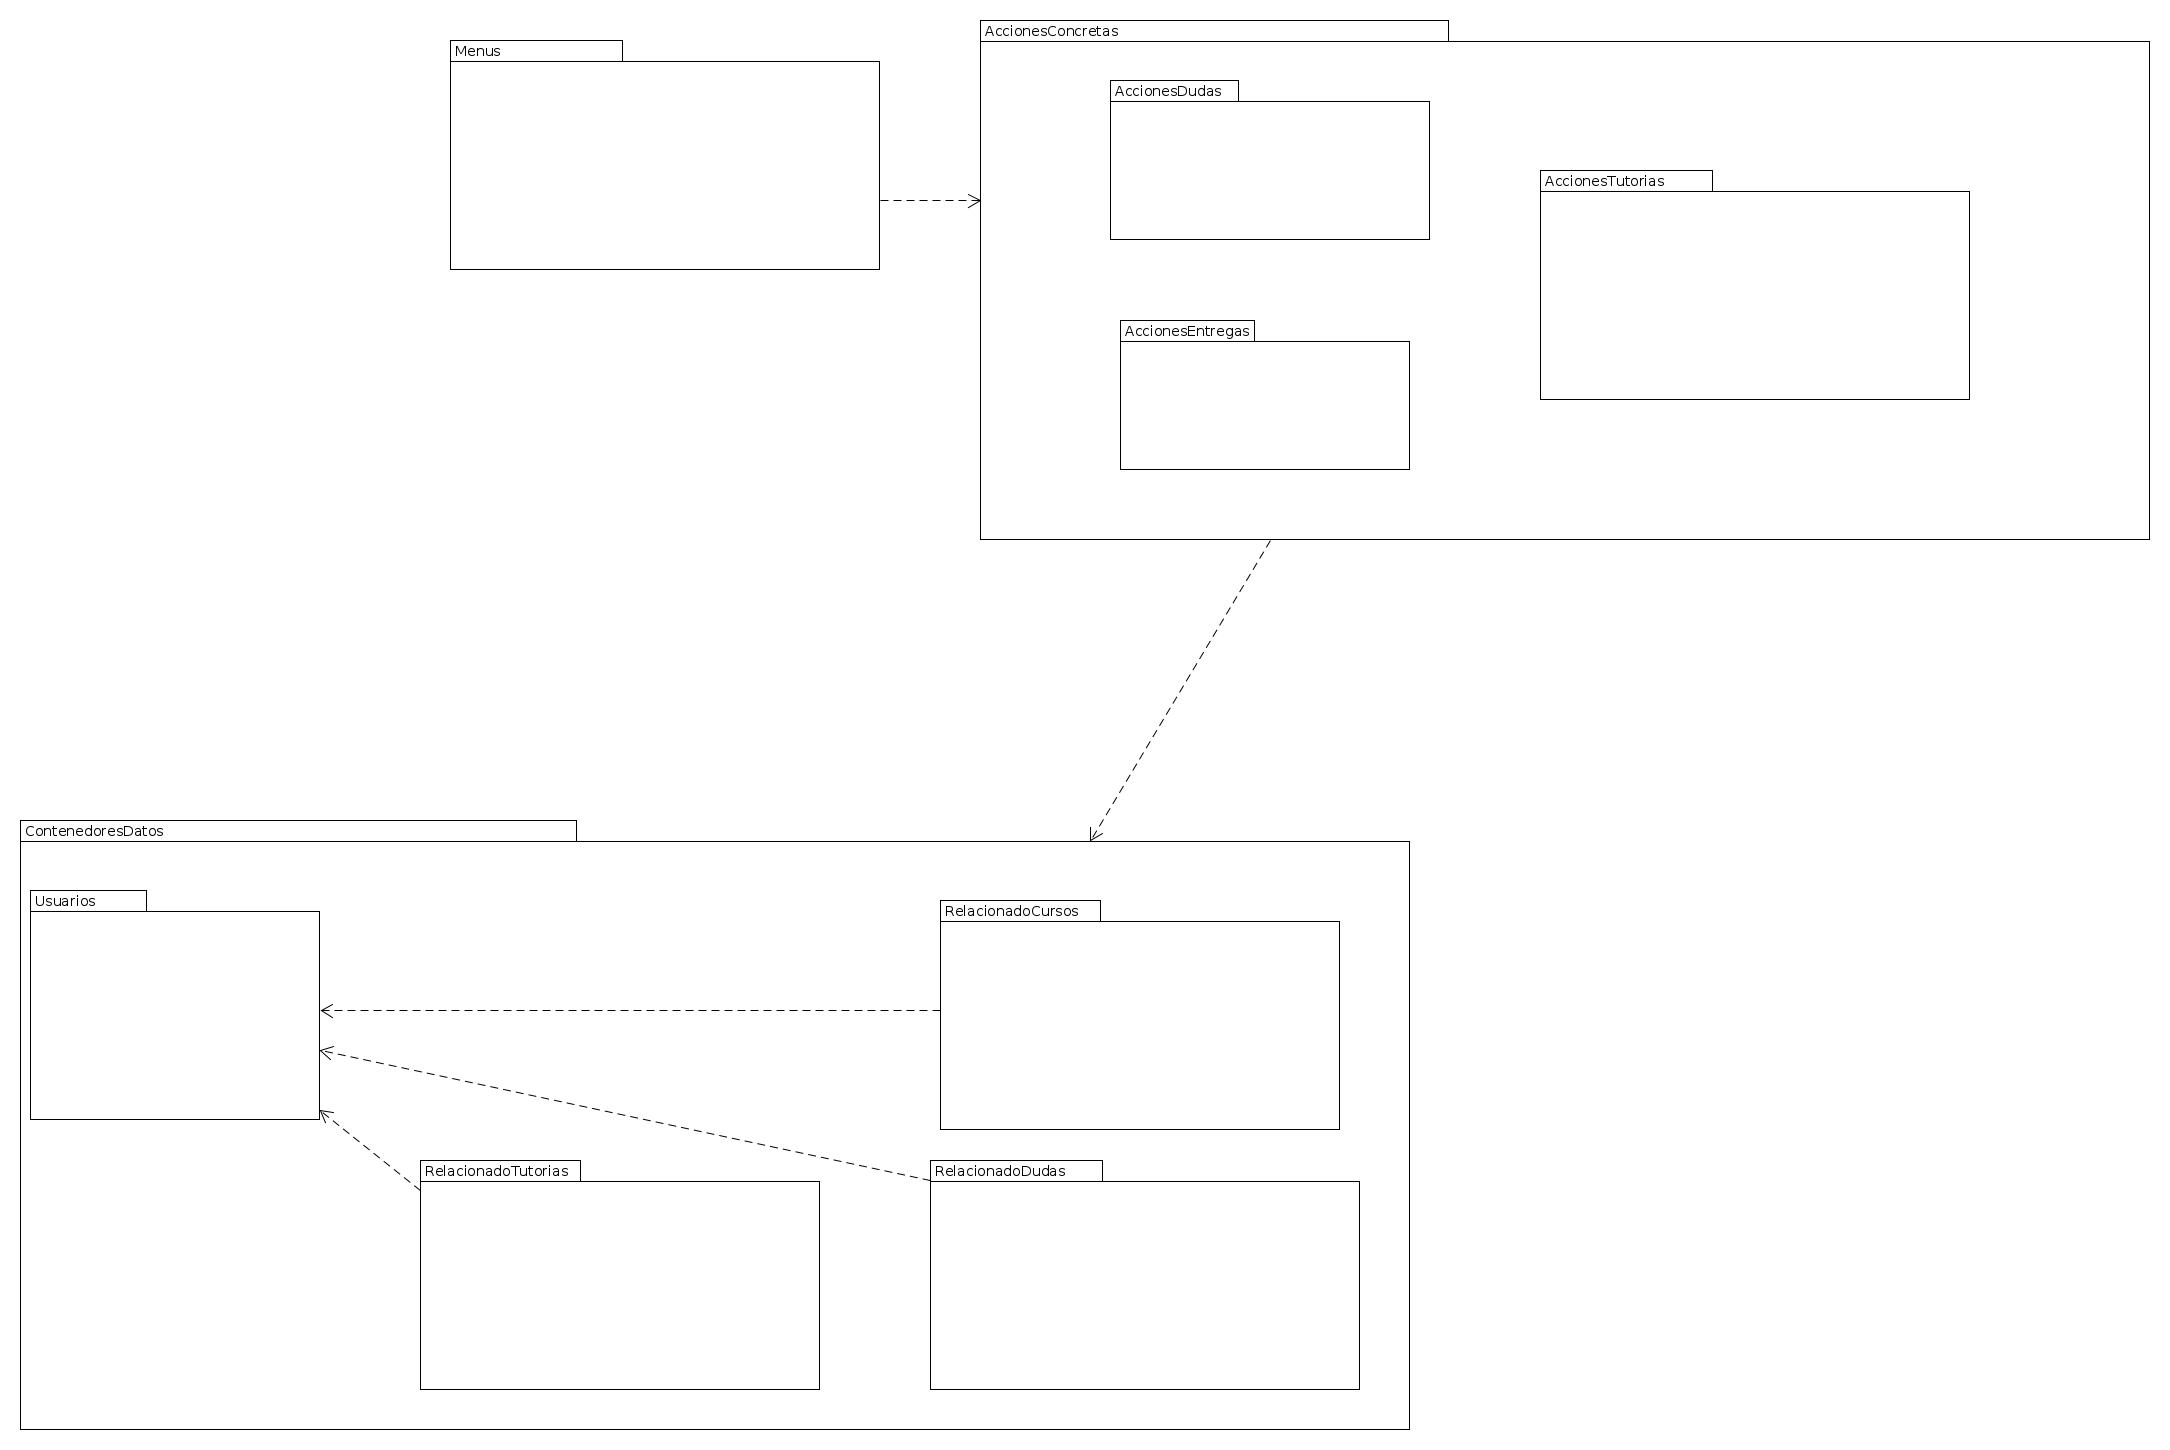
\includegraphics[scale=0.2]{imagenes/diagramas/diagrama_de_paquetes.png}  %el parámetro scale permite agrandar o achicar la imagen. En el nombre de archivo puede especificar directorios

\caption{Diagrama de paquetes del sistema}\label{figura20}
\end{figure}

    
    %%%%%%%%%%%%%%%%%%%%%%%%%%%%%%%%%%%%%%%%%
    
    \newpage
    
   \subsection{Diagramas de actividad}

A continuación mostramos los diagramas de actividad para representar el flujo de procesos contenidos en los CU.

    \begin{figure}[!ht] %con el [!ht] le obligamos a situar aquí la figura
\centering
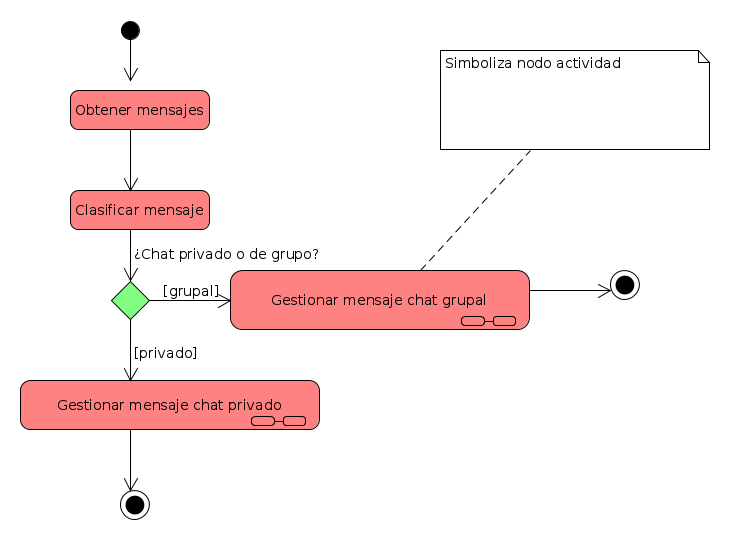
\includegraphics[scale=0.5]{imagenes/diagramas/actividad/clasificar_mensaje.png}  %el parámetro scale permite agrandar o achicar la imagen. En el nombre de archivo puede especificar directorios

\caption{Diagrama actividad CU-1.1 Clasificar mensaje}\label{figura111}
\end{figure}

    \begin{figure}[!ht] %con el [!ht] le obligamos a situar aquí la figura
\centering
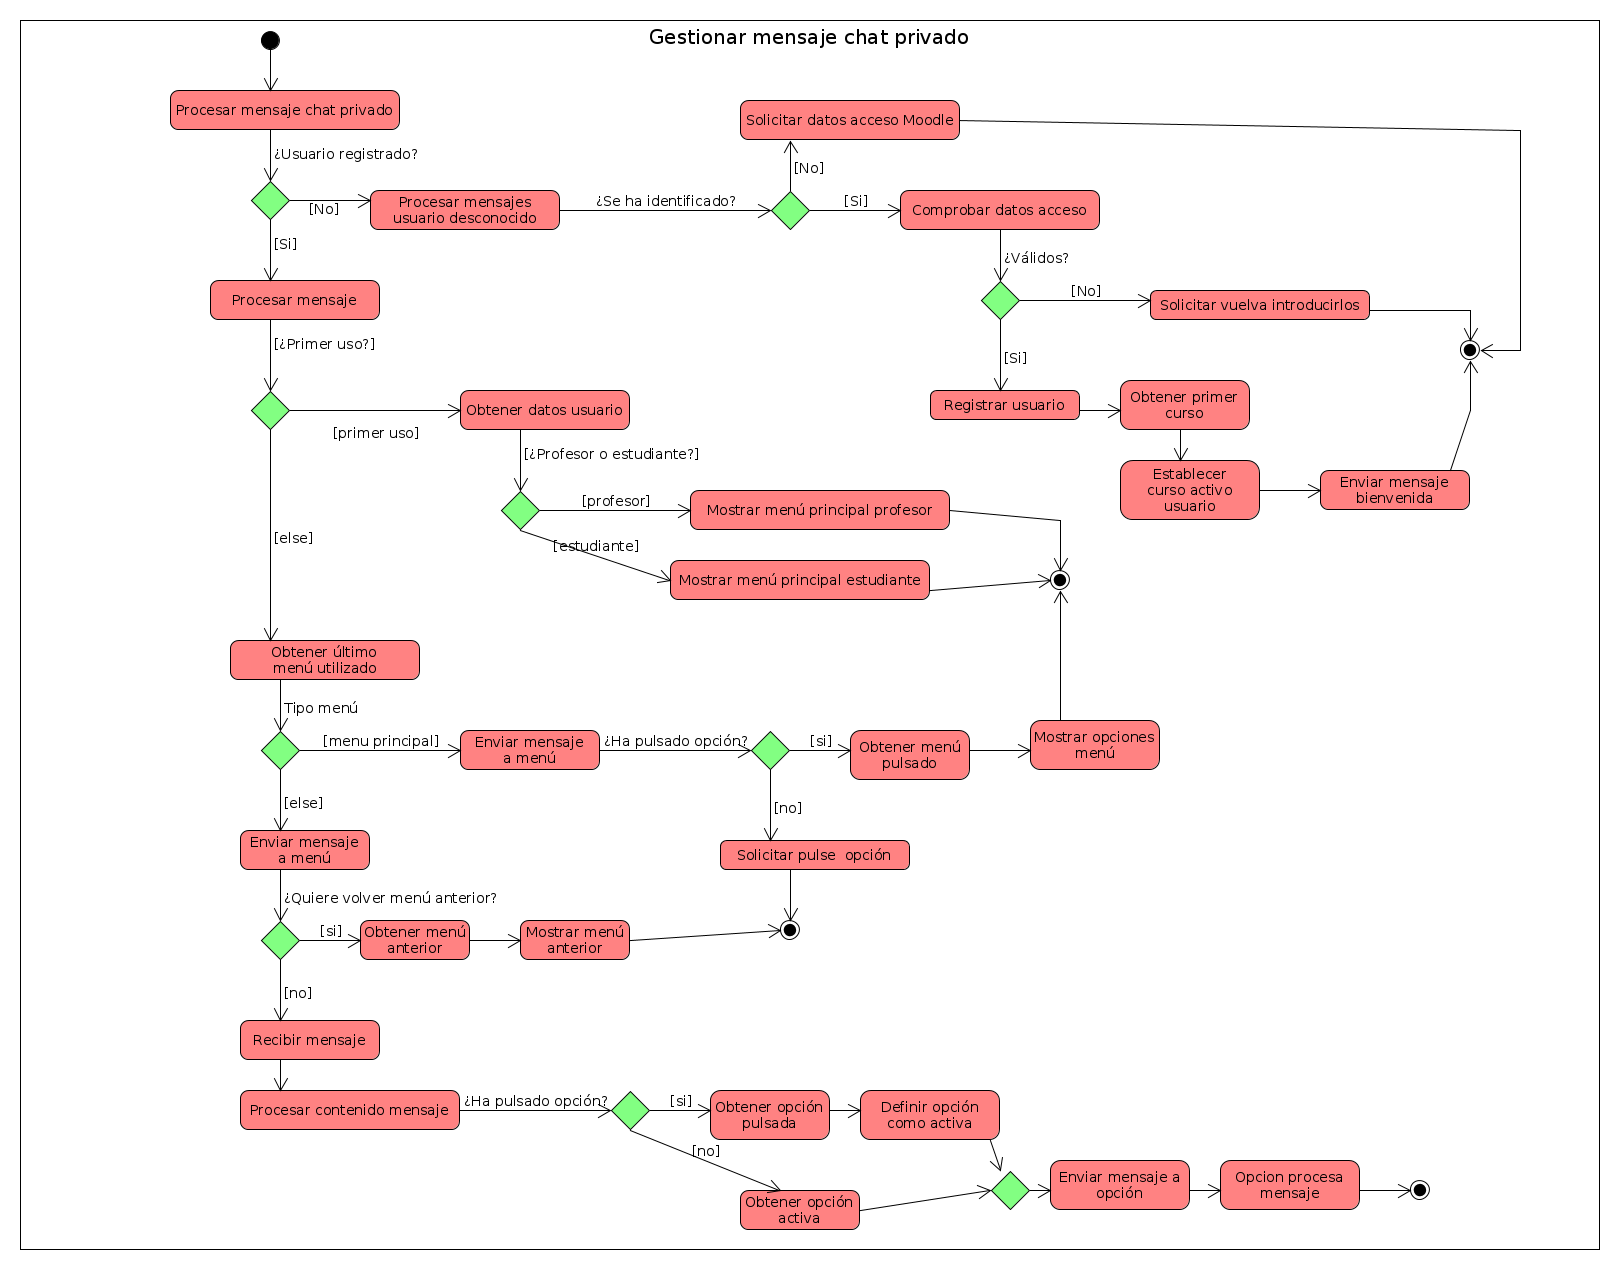
\includegraphics[scale=0.2]{imagenes/diagramas/actividad/mensaje_chat_privadoo.png}  %el parámetro scale permite agrandar o achicar la imagen. En el nombre de archivo puede especificar directorios

\caption{Diagrama actividad CU-1.2 Clasificar mensaje privado}\label{figura131}
\end{figure}
    

        \begin{figure}[!ht] %con el [!ht] le obligamos a situar aquí la figura
\centering
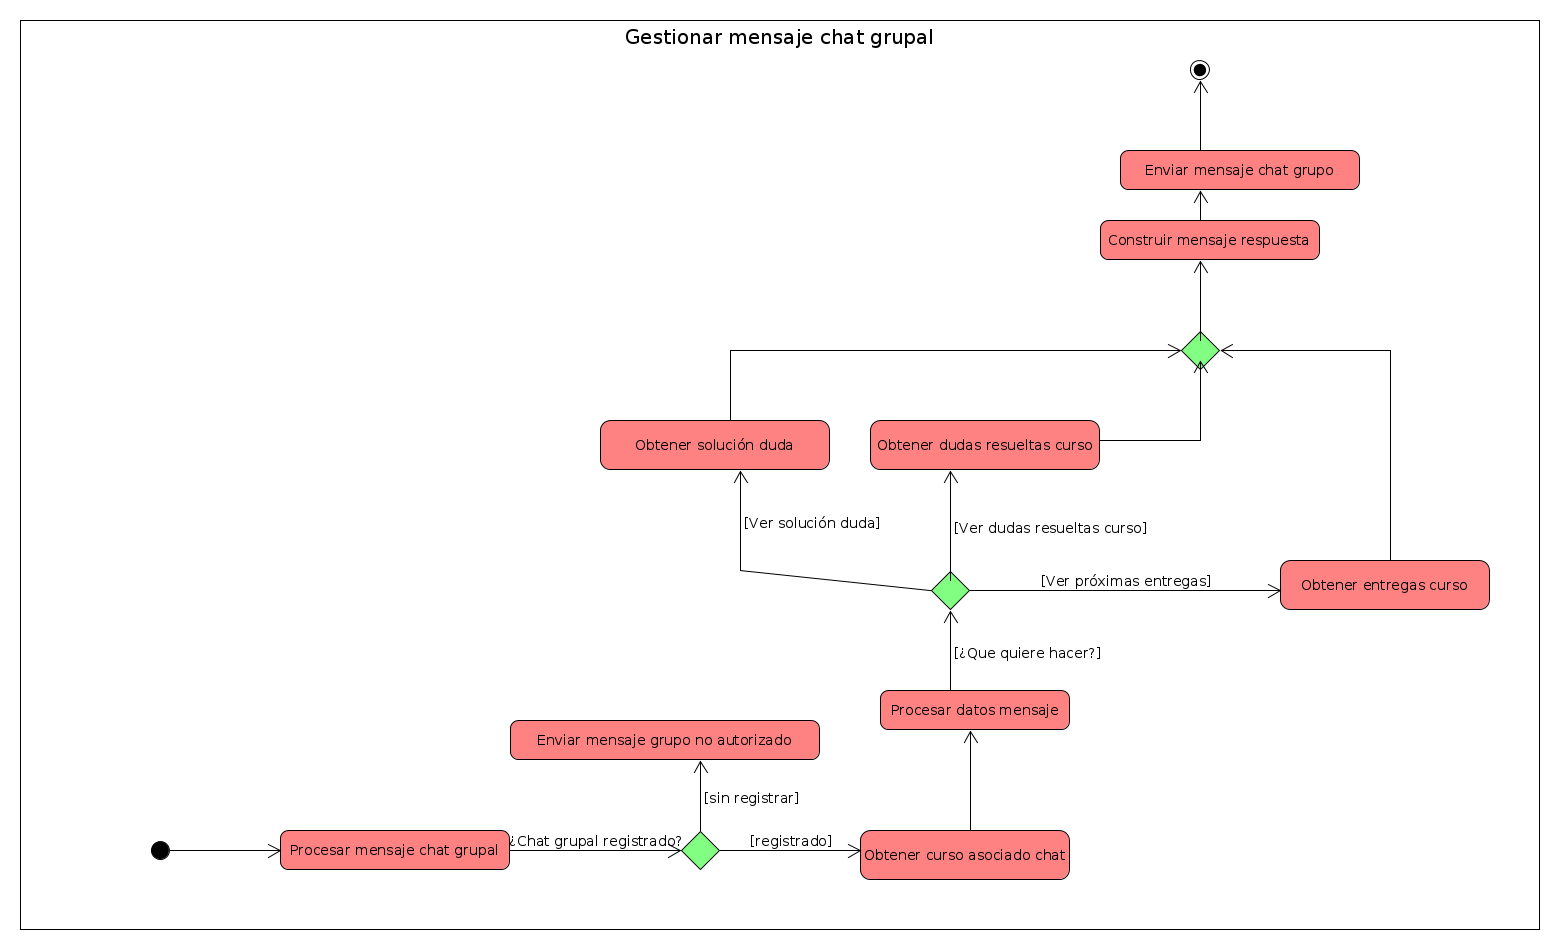
\includegraphics[scale=0.25]{imagenes/diagramas/actividad/mensaje_chat_grupall.png}  %el parámetro scale permite agrandar o achicar la imagen. En el nombre de archivo puede especificar directorios

\caption{Diagrama actividad CU-7.1, CU-7.2, CU-7.3  Mostrar solución duda, mostrar dudas resueltas y entregas por chat grupal}\label{figura141}
\end{figure}

A continucación mostramos los diagramas de actividad de los CU relacionados con las tutorías.

        \begin{figure}[!ht] %con el [!ht] le obligamos a situar aquí la figura
\centering
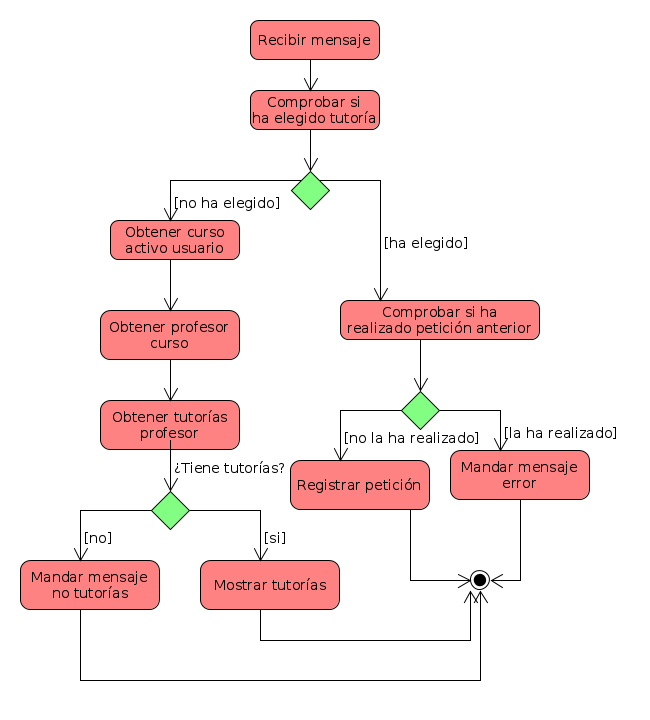
\includegraphics[scale=0.5]{imagenes/diagramas/actividad/realizar_peticon_tutoriaa.png}  %el parámetro scale permite agrandar o achicar la imagen. En el nombre de archivo puede especificar directorios

\caption{Diagrama actividad de CU-4.3 Solicitar tutoría}\label{figura143}
\end{figure}

        \begin{figure}[!ht] %con el [!ht] le obligamos a situar aquí la figura
\centering
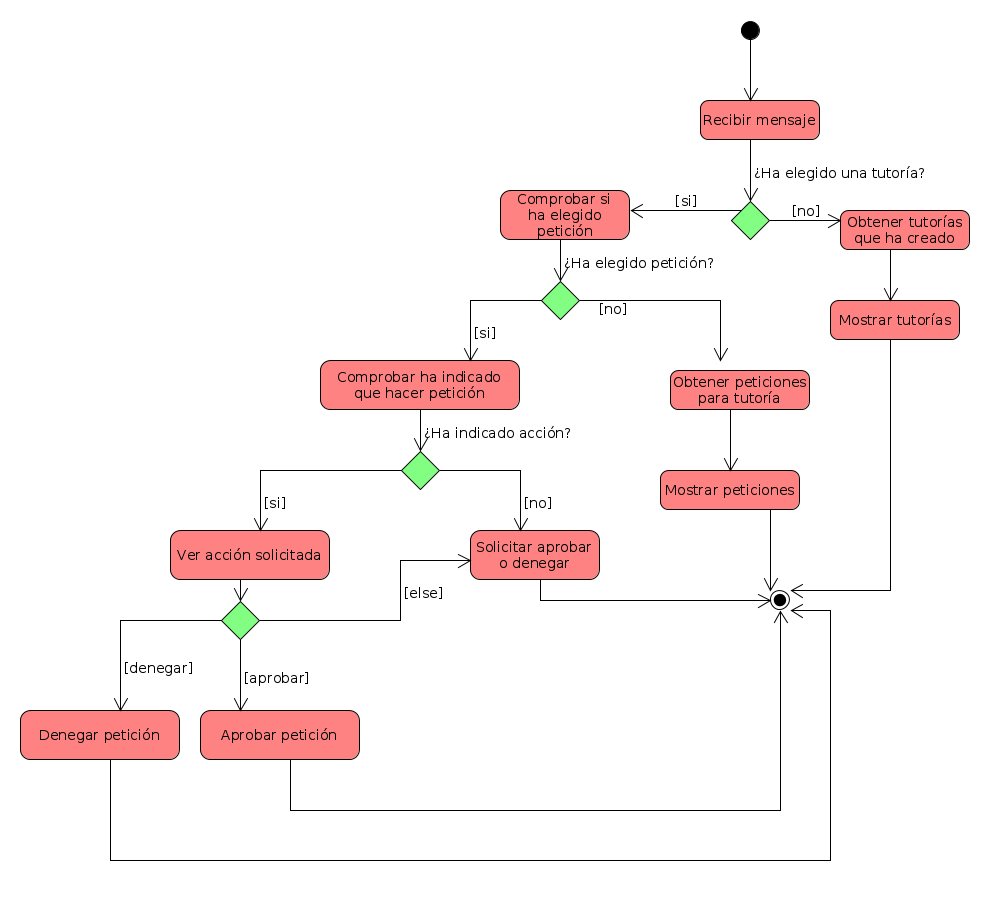
\includegraphics[scale=0.3]{imagenes/diagramas/actividad/aprobar_denegar_peticiones.png}  %el parámetro scale permite agrandar o achicar la imagen. En el nombre de archivo puede especificar directorios

\caption{Diagrama actividad conjunto de CU-4.4 Aceptar petición tutoría, CU-4.5 Denegar petición tutoría}\label{figura144}
\end{figure}

        \begin{figure}[!ht] %con el [!ht] le obligamos a situar aquí la figura
\centering
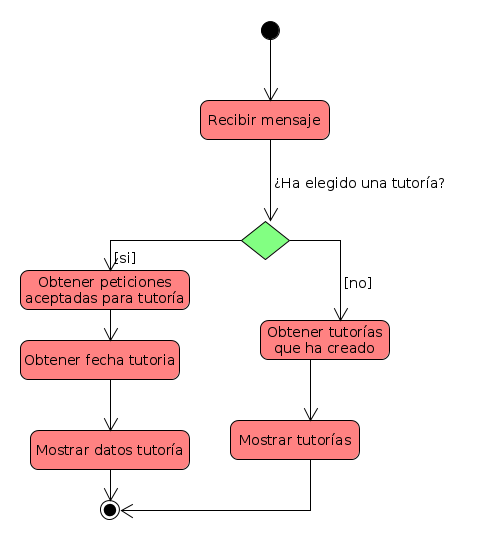
\includegraphics[scale=0.5]{imagenes/diagramas/actividad/cola_tutorias.png}  %el parámetro scale permite agrandar o achicar la imagen. En el nombre de archivo puede especificar directorios

\caption{Diagrama actividad  de CU-4.6 Ver información tutoría}\label{figura145}
\end{figure}



        \begin{figure}[!ht] %con el [!ht] le obligamos a situar aquí la figura
\centering
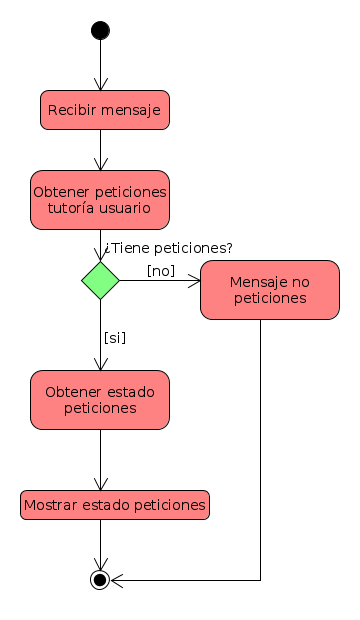
\includegraphics[scale=0.5]{imagenes/diagramas/actividad/ver_peticiones_realizadass.png}  %el parámetro scale permite agrandar o achicar la imagen. En el nombre de archivo puede especificar directorios

\caption{Diagrama actividad de CU-4.7 Ver peticiones realizadas}\label{figura147}
\end{figure}

        \begin{figure}[!ht] %con el [!ht] le obligamos a situar aquí la figura
\centering
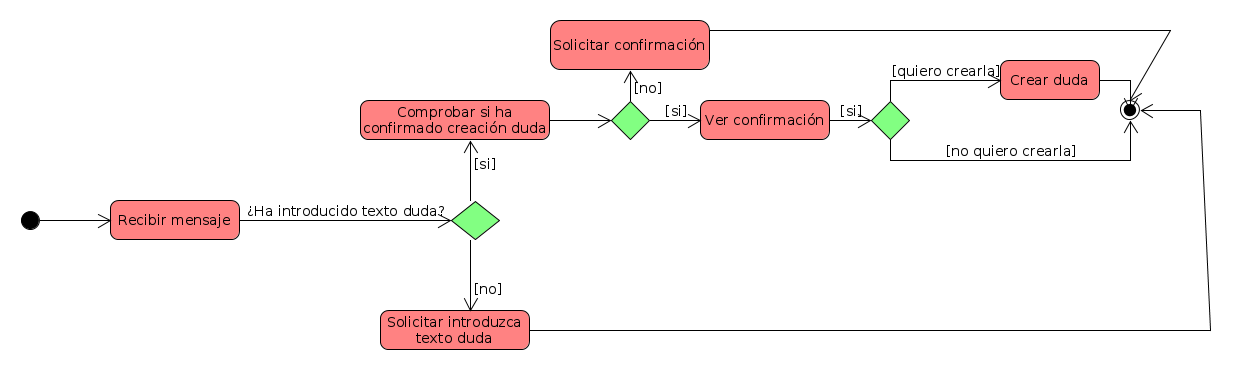
\includegraphics[scale=0.3]{imagenes/diagramas/actividad/crear_duda.png}  %el parámetro scale permite agrandar o achicar la imagen. En el nombre de archivo puede especificar directorios

\caption{Diagrama actividad de CU-5.1 Crear duda}\label{figura148}
\end{figure}

        \begin{figure}[!ht] %con el [!ht] le obligamos a situar aquí la figura
\centering
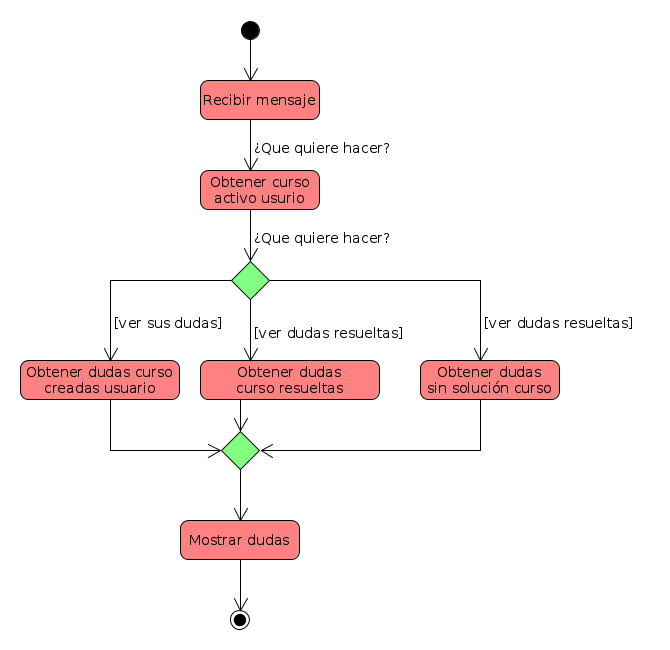
\includegraphics[scale=0.3]{imagenes/diagramas/actividad/ver_dudas_sin_con_mis.png}  %el parámetro scale permite agrandar o achicar la imagen. En el nombre de archivo puede especificar directorios

\caption{Diagrama actividad conjunto de CU-5.2 Ver dudas sin solución, CU-5.3 Ver mis dudas, CU-5.4 Ver dudas resueltas,}\label{figura1423}
\end{figure}


        \begin{figure}[!ht] %con el [!ht] le obligamos a situar aquí la figura
\centering
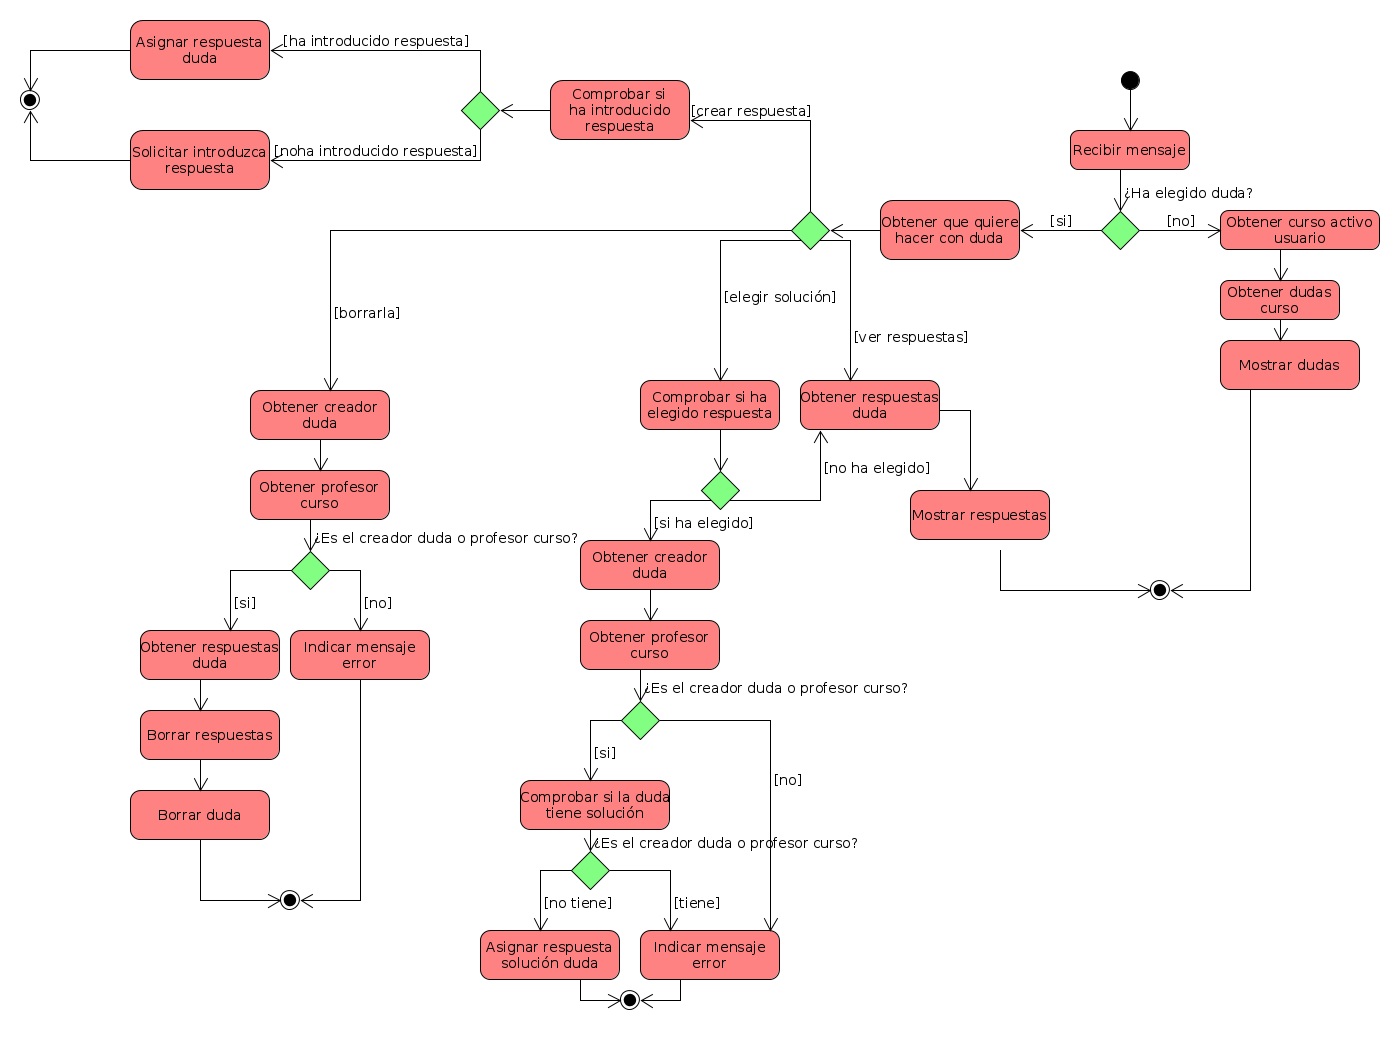
\includegraphics[scale=0.2]{imagenes/diagramas/actividad/operaciones_dudaa.png}  %el parámetro scale permite agrandar o achicar la imagen. En el nombre de archivo puede especificar directorios

\caption{Diagrama actividad conjunto de  CU-5.5 Crear respuesta a duda, CU-5.6 Ver respuesta duda, CU-5.7 Ver solución duda, CU-5.8 Borrar mi duda, CU-5.9 Elegir solución mi duda, CU-10 Borrar duda, CU-11 Elegir solución a duda}\label{figura151}
\end{figure}

        \begin{figure}[!ht] %con el [!ht] le obligamos a situar aquí la figura
\centering
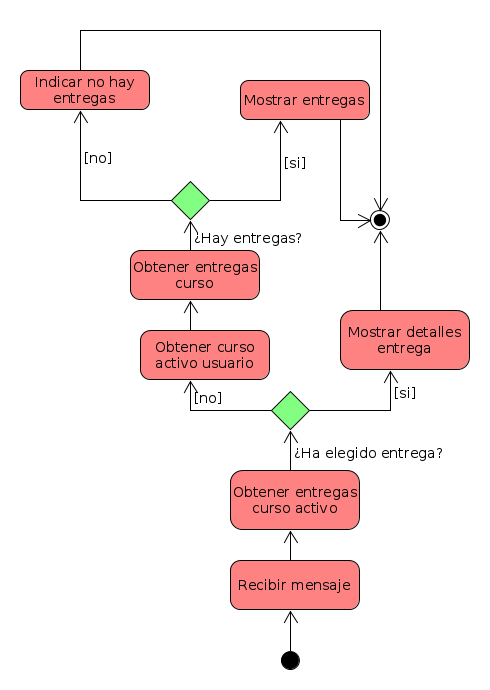
\includegraphics[scale=0.4]{imagenes/diagramas/actividad/mostrar_entregass.png}  %el parámetro scale permite agrandar o achicar la imagen. En el nombre de archivo puede especificar directorios

\caption{Diagrama actividad CU-6.1 Ver entregas}\label{figura153}
\end{figure}

        \begin{figure}[!ht] %con el [!ht] le obligamos a situar aquí la figura
\centering
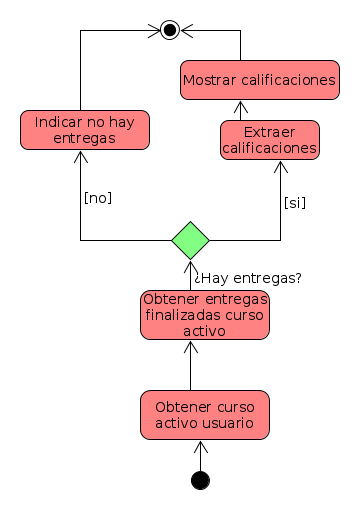
\includegraphics[scale=0.4]{imagenes/diagramas/actividad/mostrar_calificaciones.png}  %el parámetro scale permite agrandar o achicar la imagen. En el nombre de archivo puede especificar directorios

\caption{Diagrama actividad CU-6.2 Mostrar calificaciones}\label{figura152}
\end{figure}



    